\onecolumn
\newpage
\definecolor{question_color}{RGB}{0,100,0}
\appendix
\section{Appendix}
\subsection{Additional Related Works}
\label{apdx:additional_related}
Additional works also mitigate the challenges posed by massive KV Caches during long-sequence inference while not reducing the number of cache elements. These works are orthogonal to our work. For instance, in our implementation, we have integrated the Flash Attention~\cite{dao2022flashattention} technique to enhance efficient computation. Similar efforts, such as Paged Attention~\cite{kwon2023efficient}, employ efficient memory management strategies to reduce I/O latency without altering the size of the KV Cache.
KV cache quantization methods~\cite{yao2022zeroquant,liu2024kivi,dong2024qaq}, reduce the size of cache by lowering the precision of individual elements. The cache eviction techniques focused in this paper also be further combined and complemented with quantization in the future. 
Some studies also employ speculative decoding to accelerate long-sequence generation~\cite{sun2024triforce, yanglongspec, ji2025specvlm}, typically using model with a reduced KV cache to generate drafts. Future work could integrate more advanced cache eviction methods to further improve the efficiency of such approaches.




\subsection{Detail results of Ruler Evaluation}
\label{apdx:detail_ruler}
Figure~\ref{fig:ruler_llama_mqa} complements the missing result for the multi-hop QA subtask in Figure~\ref{fig:agnostic_llama_ruler_subtask} due to the space limitation. Figures~\ref{fig:agnostic_mistral_ruler_subtask}~\ref{fig:aware_llama_ruler_subtask}~\ref{fig:aware_mistral_ruler_subtask} further provide a comprehensive overview of the performance of Ada-SnapKV and Ada-Pyramid across all 16K Ruler subtasks on two LLMs in both question-agnostic and question-aware scenarios. The results demonstrate that regardless of the scenario (question-agnostic or question-aware), model (LLama or Mistral), or cache size budgets, Ada-SnapKV and Ada-Pyramid outperform the original SnapKV and Pyramid approaches in most tasks. This highlights the broad applicability and effectiveness of the adaptive allocation strategy.

\begin{figure}[h]
	\centering
	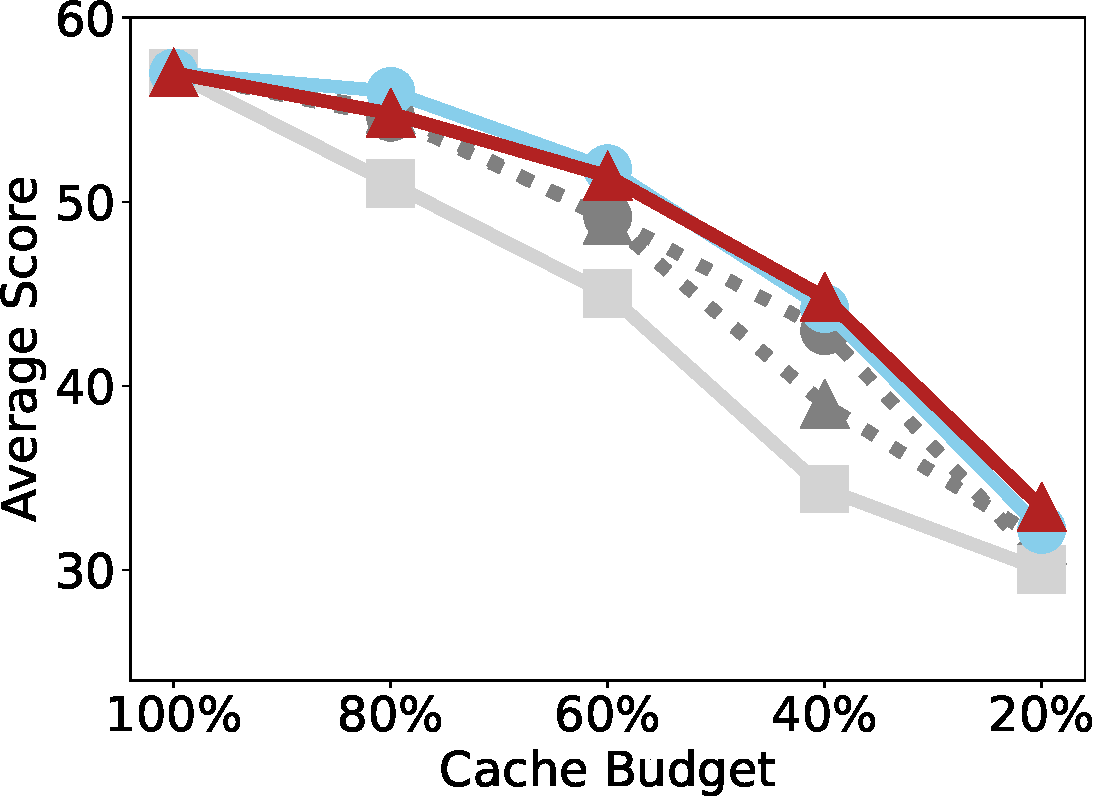
\includegraphics[width=0.25\linewidth]{./Figures/ruler_per_dataset_group_by_wq/qa_2_Llama3.1_ruler_score.pdf}
	\caption{M-QA Subtask Analysis on Ruler for Question-agnostic Scenario (Llama3.1-8B-Instruct)}
	\label{fig:ruler_llama_mqa}
\end{figure}


\subsection{Robustness Analysis of Safeguard $\alpha$}

Rather than fine-tuning the safeguard parameter, $\alpha$, for each model or budget—a process that would introduce considerable complexity—we opted for a fixed value. As shown in Table [Table Number], we conducted a robustness analysis of $\alpha$ using Mistral-7B on the LongBench benchmark.
The results indicate that a smaller $\alpha$ allows for more aggressive budget allocation, improving performance under limited budgets. Conversely, a larger $\alpha$ performs slightly better with higher budgets. Based on this trade-off, we selected a balanced value for $\alpha=0.2$ in this work.


\begin{table}[h!]
	\centering
	\small
	\caption{Robustness Analysis of $\alpha$ (Question-aware)}
	
	\begin{tabular}{lcccc}
		\toprule Longbench, Mistral-7B
		& {Budget 128} & {Budget 256} & {Budget 512} & {Budget 1024} \\
		\midrule
		Ada-SnapKV $\alpha=0$ & \textbf{35.69} & \textbf{38.9} & 40.53 & 41.44 \\
		Ada-SnapKV $\alpha=0.2$ & 35.48 & 38.61 & 40.58 & 41.61 \\
		Ada-SnapKV $\alpha=0.5$ & 35.2 & 38.46 & \textbf{40.66} & \textbf{41.62} \\
		\bottomrule
	\end{tabular}
\end{table}

\begin{figure*}[h!]
	\begin{minipage}{\linewidth}
	\centering
	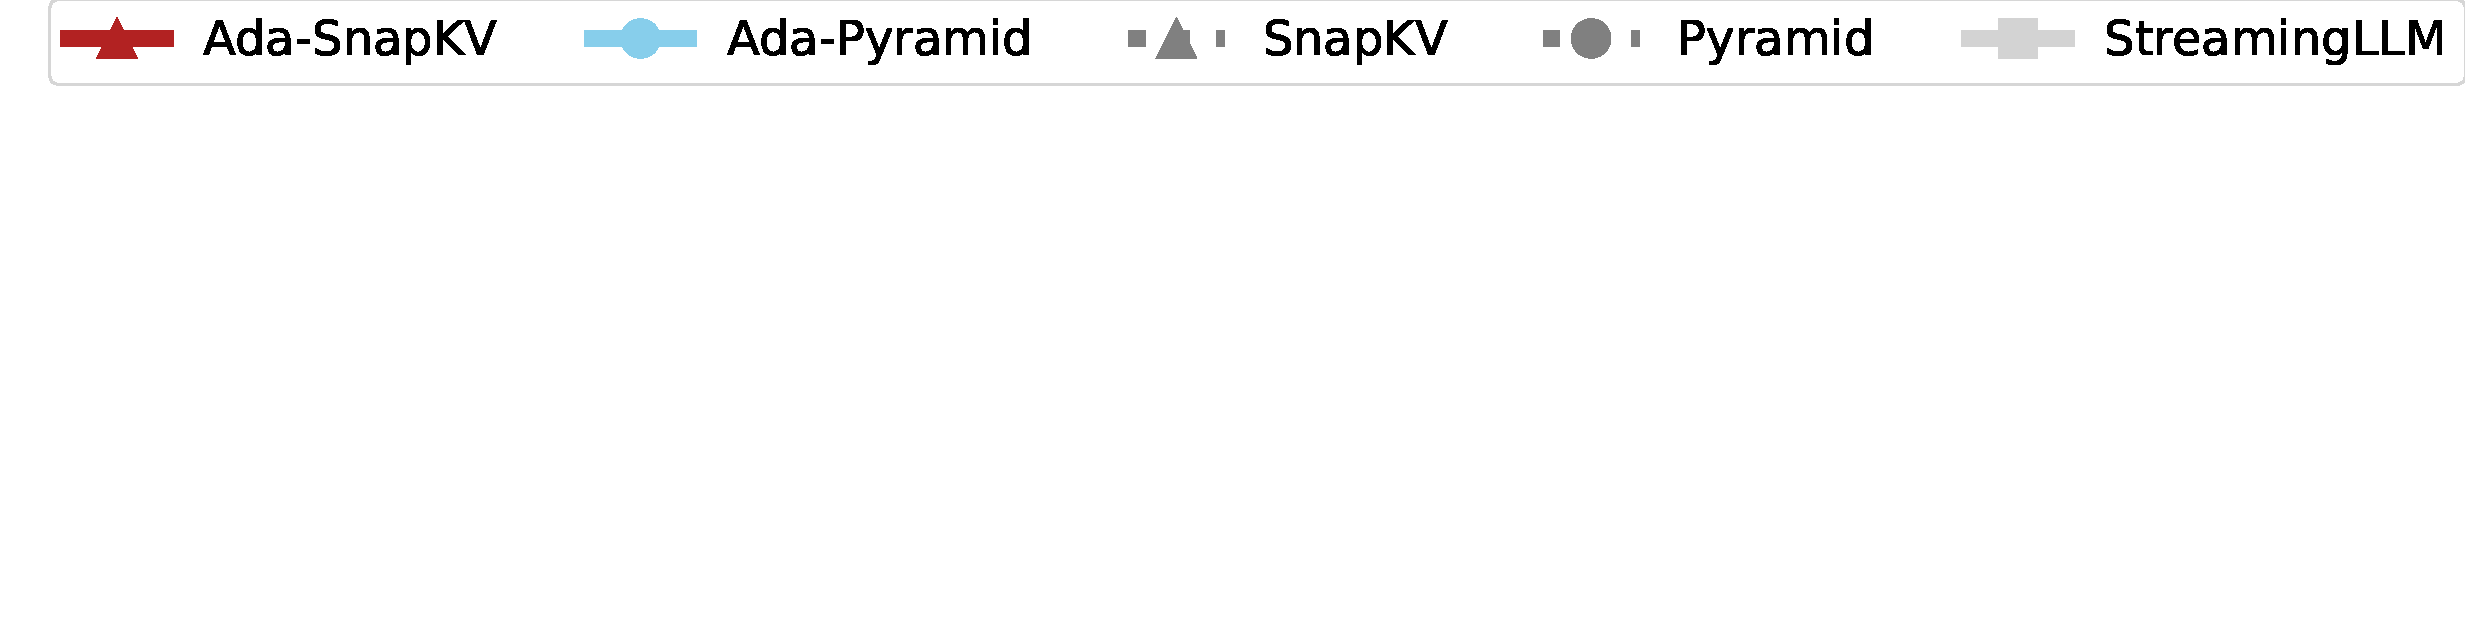
\includegraphics[width=0.7\linewidth]{./Figures/ruler_per_dataset_group_by_wq/legend.pdf} 
	\end{minipage}
	\begin{subfigure}[b]{0.16\linewidth}
		\centering
		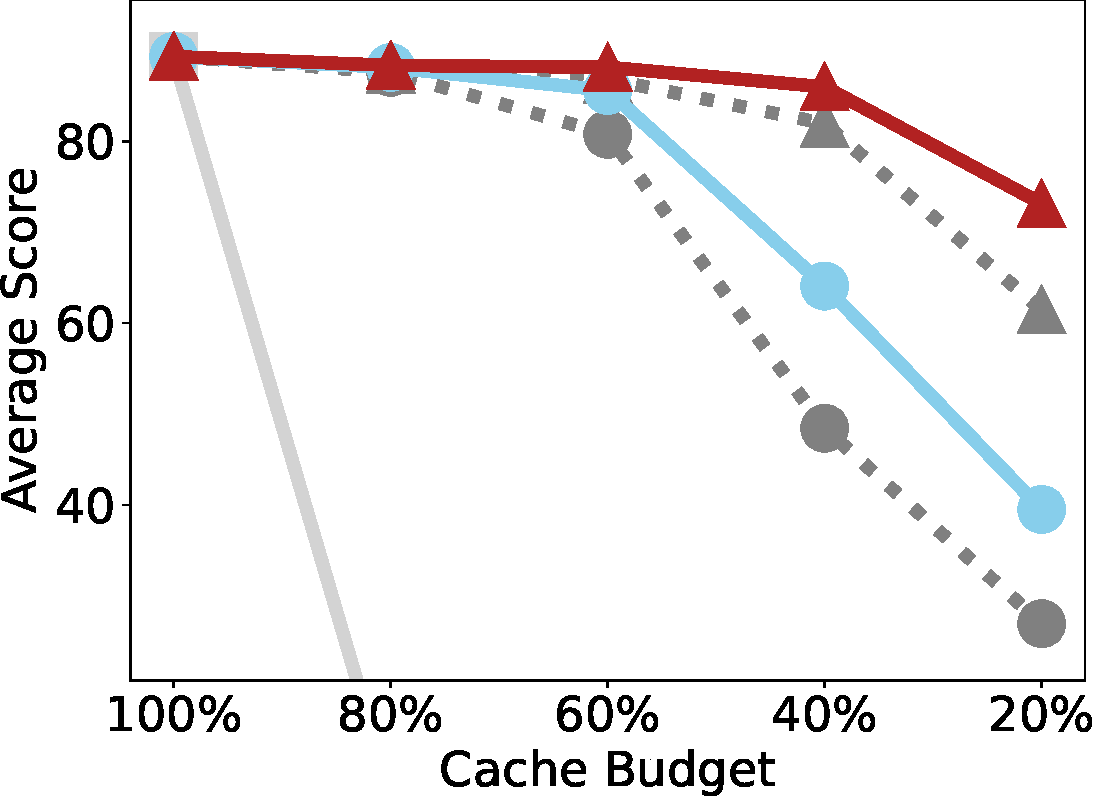
\includegraphics[width=\linewidth]{./Figures/ruler_per_dataset_group_by_wq/cwe_wq_Llama3.1_ruler_score.pdf} 
		\caption{CWE}
	\end{subfigure}
	\begin{subfigure}[b]{0.16\linewidth}
		\centering
		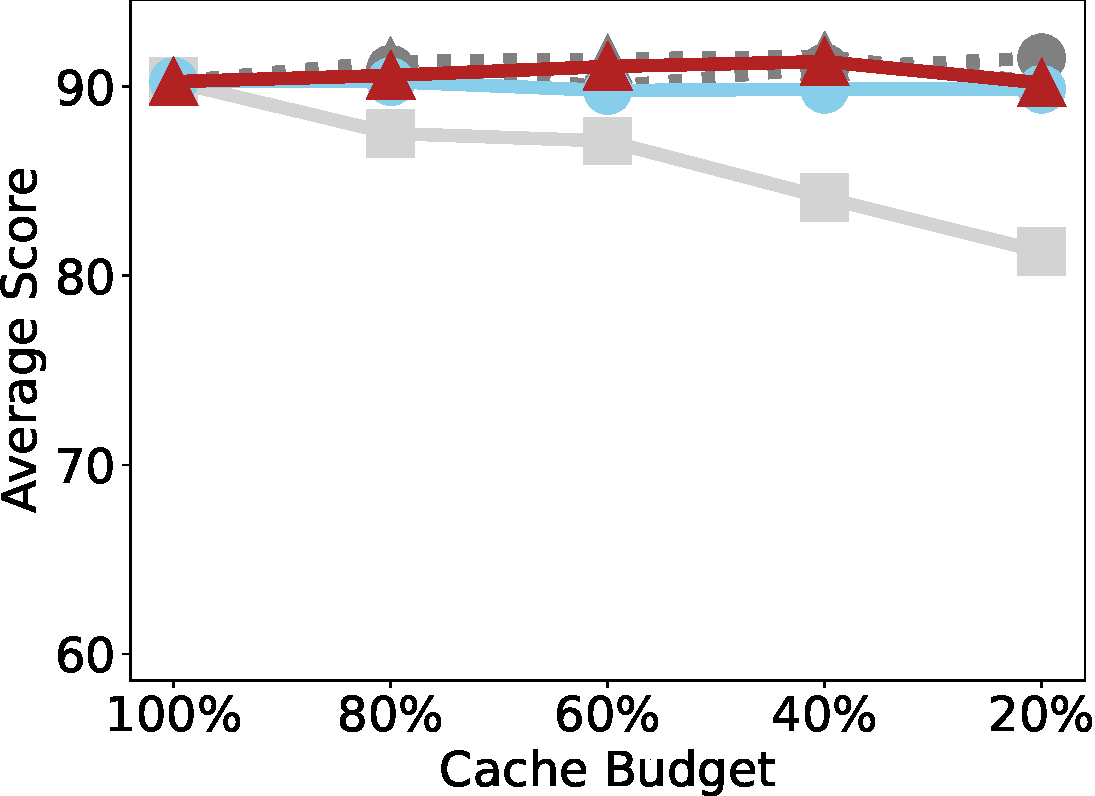
\includegraphics[width=\linewidth]{./Figures/ruler_per_dataset_group_by_wq/fwe_wq_Llama3.1_ruler_score.pdf}
		\caption{FWE}
	\end{subfigure}
	\begin{subfigure}[b]{0.16\linewidth}
		\centering
		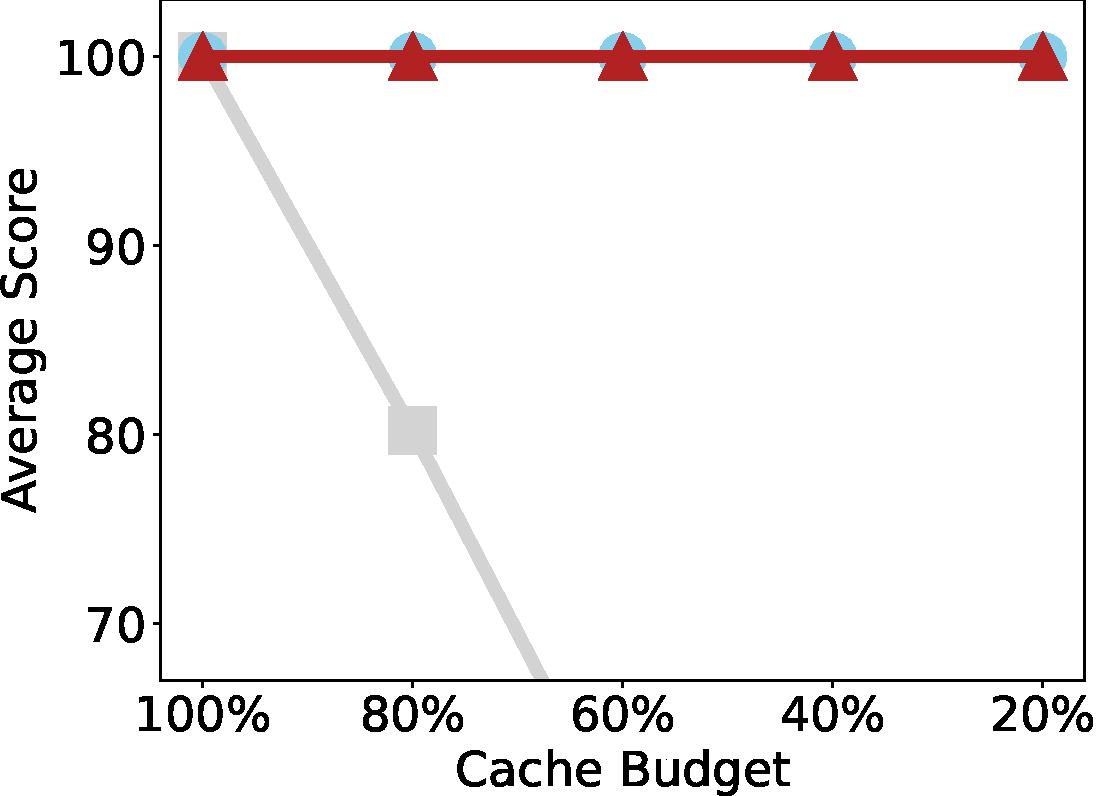
\includegraphics[width=\linewidth]{./Figures/ruler_per_dataset_group_by_wq/niah_single_1_wq_Llama3.1_ruler_score.pdf} 
		\caption{S-NIAH-1}
	\end{subfigure}
	\begin{subfigure}[b]{0.16\linewidth}
		\centering
		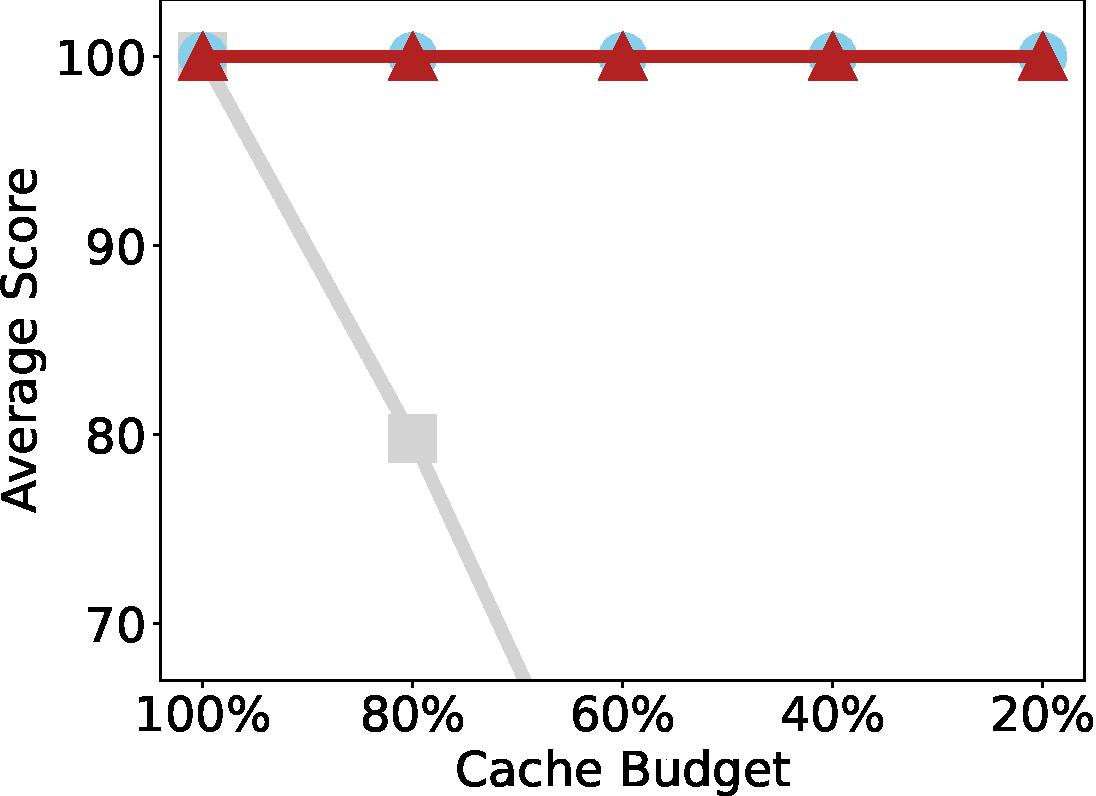
\includegraphics[width=\linewidth]{./Figures/ruler_per_dataset_group_by_wq/niah_single_2_wq_Llama3.1_ruler_score.pdf}
		\caption{S-NIAH-2}
	\end{subfigure}
	\begin{subfigure}[b]{0.16\linewidth}
		\centering
		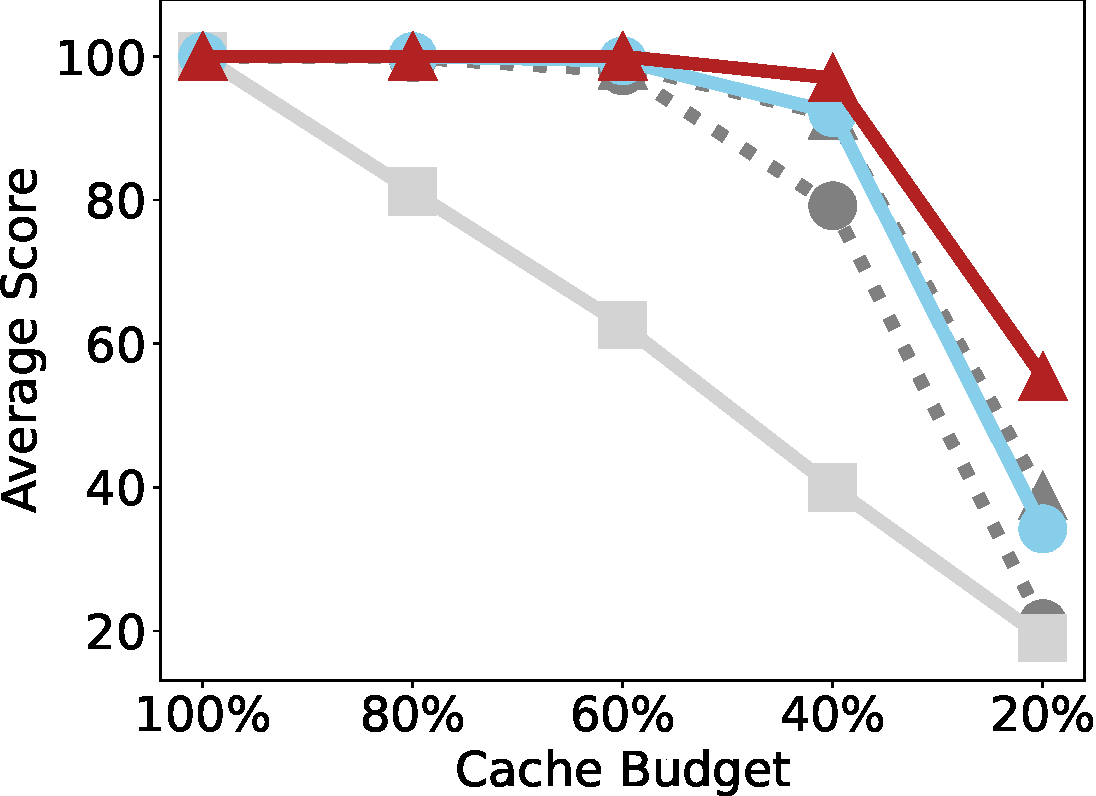
\includegraphics[width=\linewidth]{./Figures/ruler_per_dataset_group_by_wq/niah_single_3_wq_Llama3.1_ruler_score.pdf} 
		\caption{S-NIAH-3}
	\end{subfigure}
	\begin{subfigure}[b]{0.16\linewidth}
		\centering
		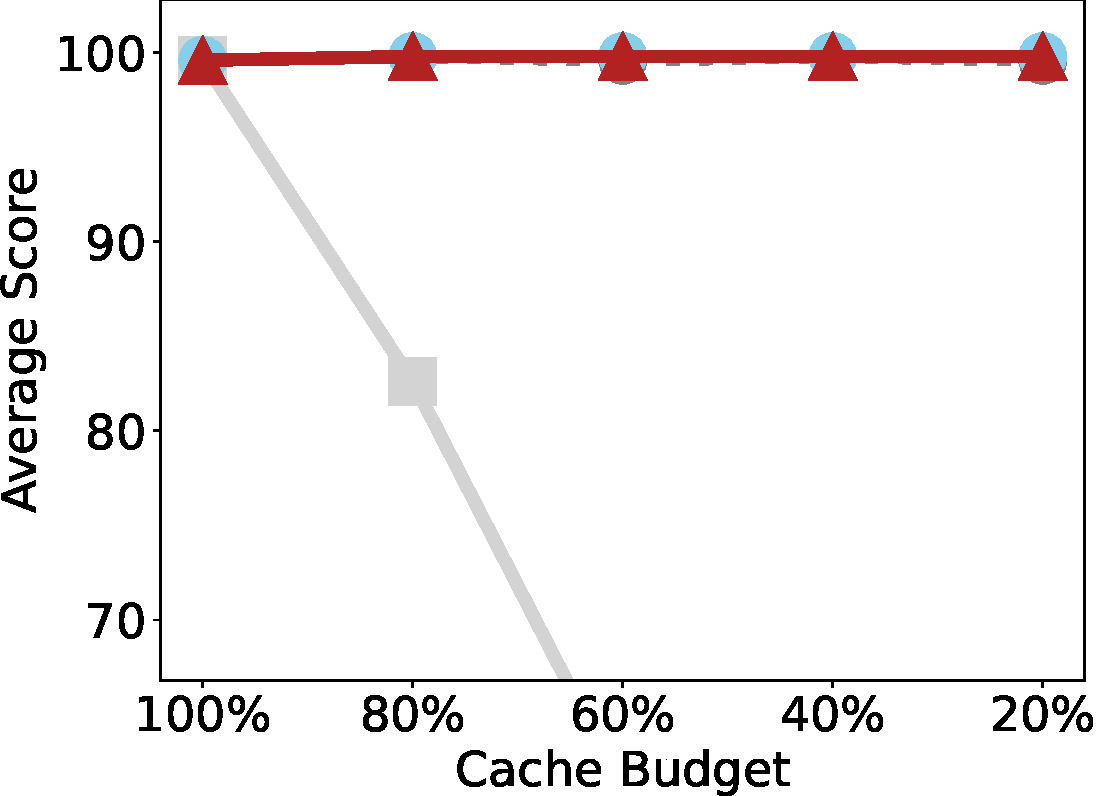
\includegraphics[width=\linewidth]{./Figures/ruler_per_dataset_group_by_wq/niah_multikey_1_wq_Llama3.1_ruler_score.pdf}
		\caption{MK-NIAH-1}
	\end{subfigure}
	\begin{subfigure}[b]{0.16\linewidth}
		\centering
		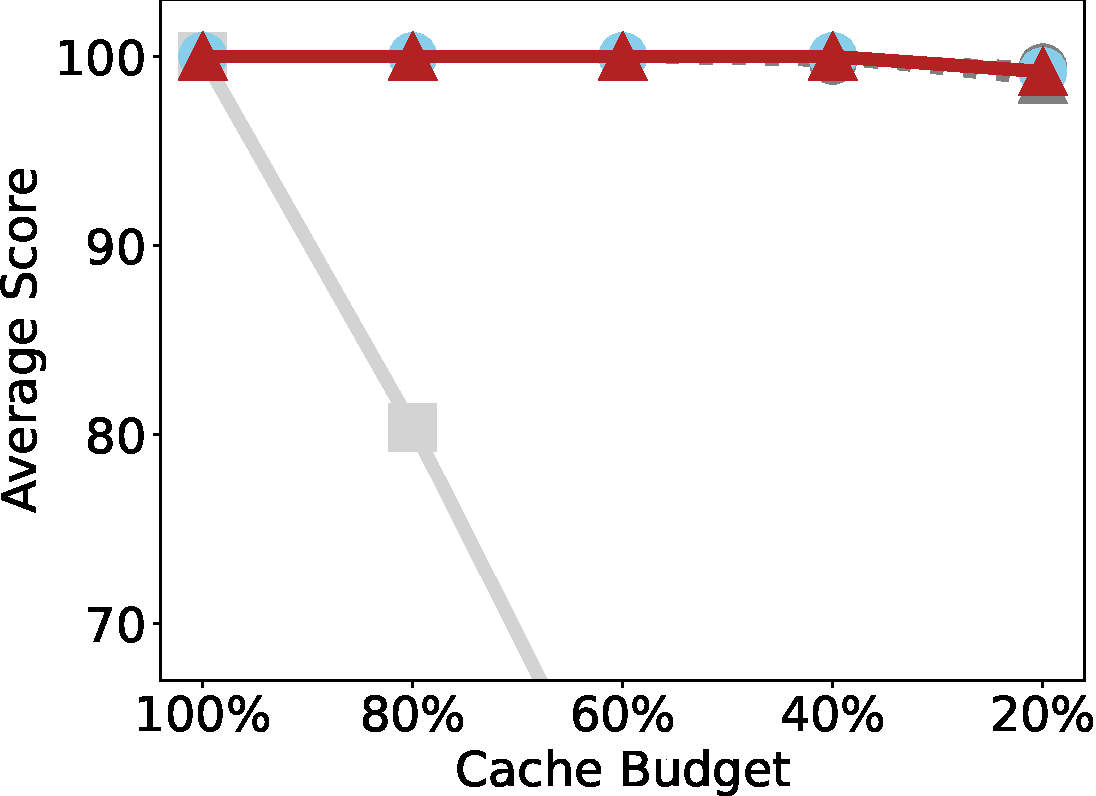
\includegraphics[width=\linewidth]{./Figures/ruler_per_dataset_group_by_wq/niah_multikey_2_wq_Llama3.1_ruler_score.pdf} 
		\caption{MK-NIAH-2}
	\end{subfigure}
	\begin{subfigure}[b]{0.16\linewidth}
		\centering
		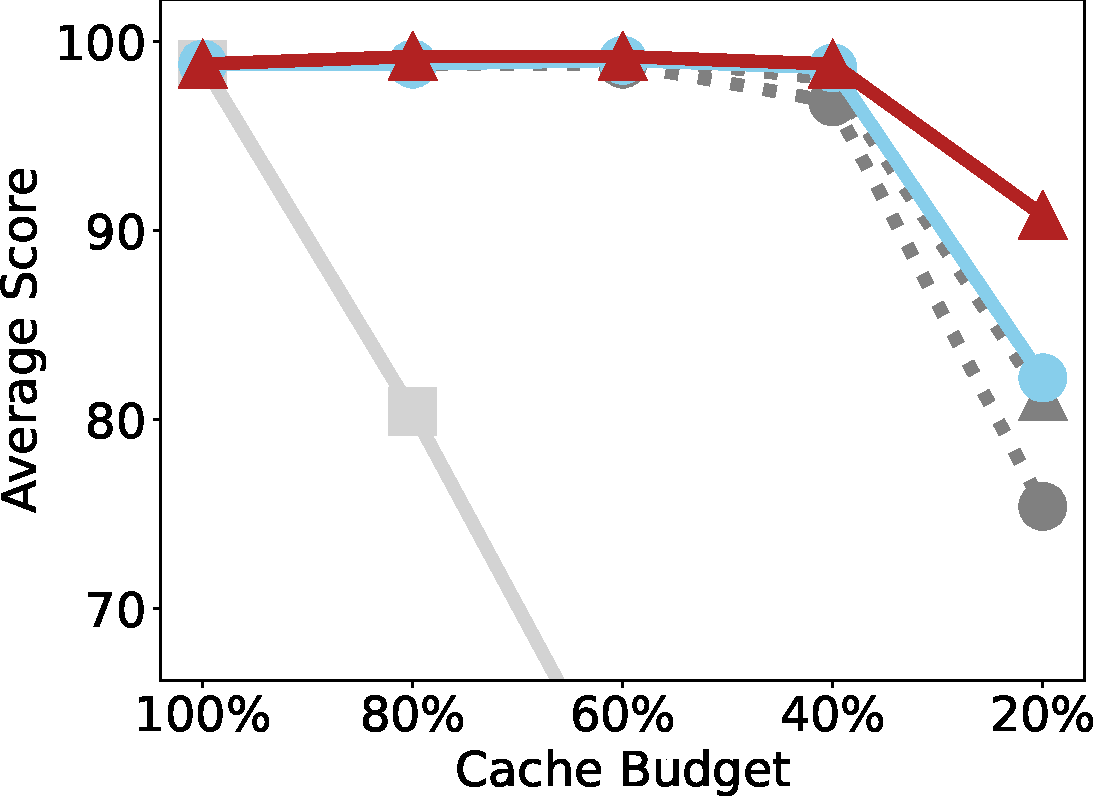
\includegraphics[width=\linewidth]{./Figures/ruler_per_dataset_group_by_wq/niah_multikey_3_wq_Llama3.1_ruler_score.pdf}
		\caption{MK-NIAH-3}
	\end{subfigure}
	\begin{subfigure}[b]{0.16\linewidth}
		\centering
		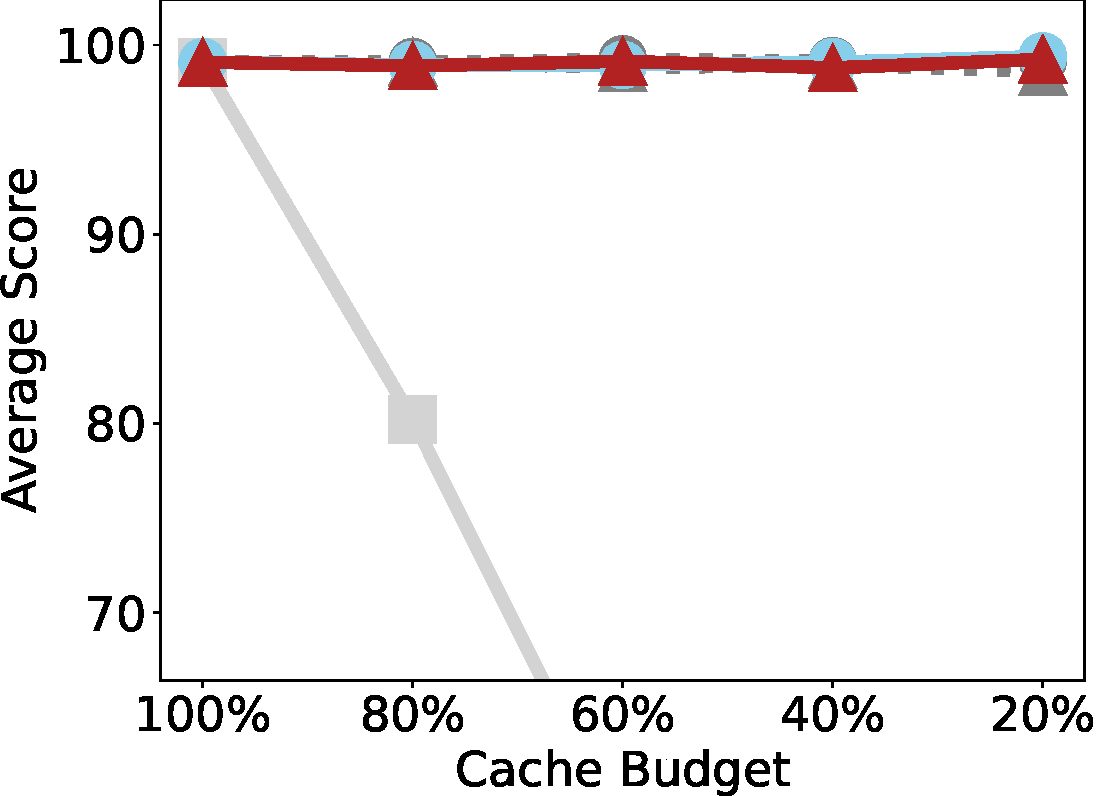
\includegraphics[width=\linewidth]{./Figures/ruler_per_dataset_group_by_wq/niah_multivalue_wq_Llama3.1_ruler_score.pdf}
		\caption{MV-NIAH}
	\end{subfigure}
	\begin{subfigure}[b]{0.16\linewidth}
		\centering
		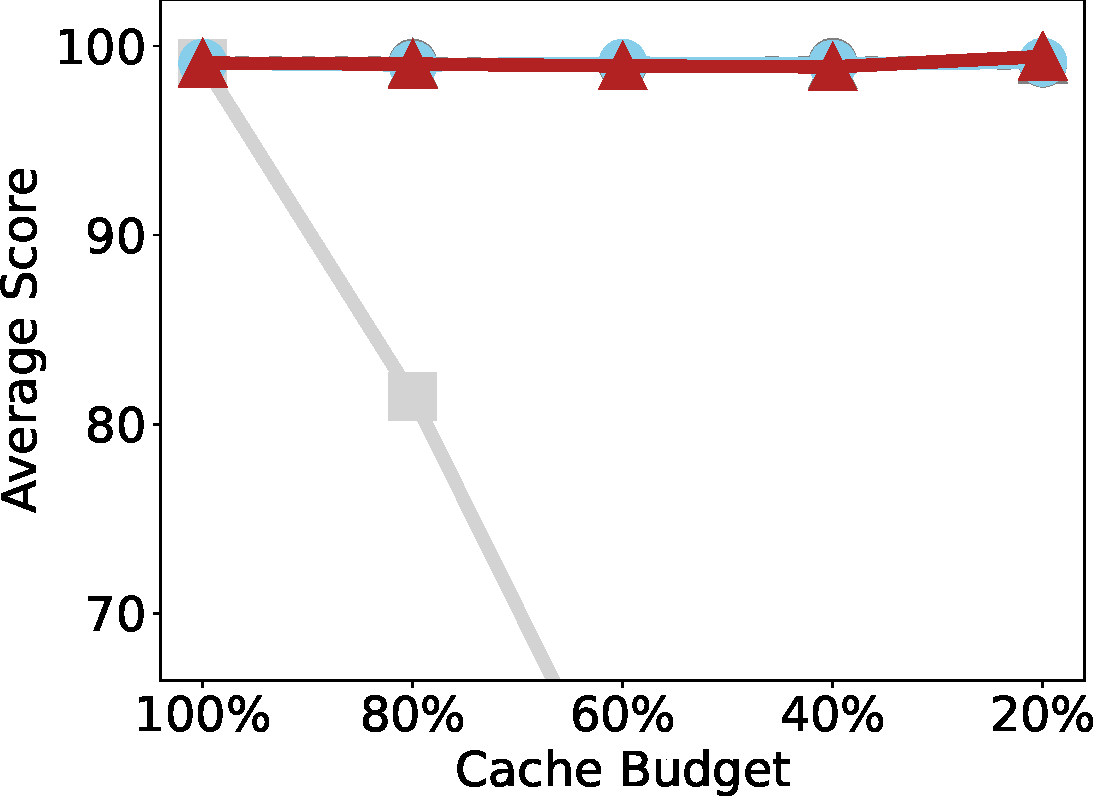
\includegraphics[width=\linewidth]{./Figures/ruler_per_dataset_group_by_wq/niah_multiquery_wq_Llama3.1_ruler_score.pdf}
		\caption{MQ-NIAH}
	\end{subfigure}
	\begin{subfigure}[b]{0.16\linewidth}
		\centering
		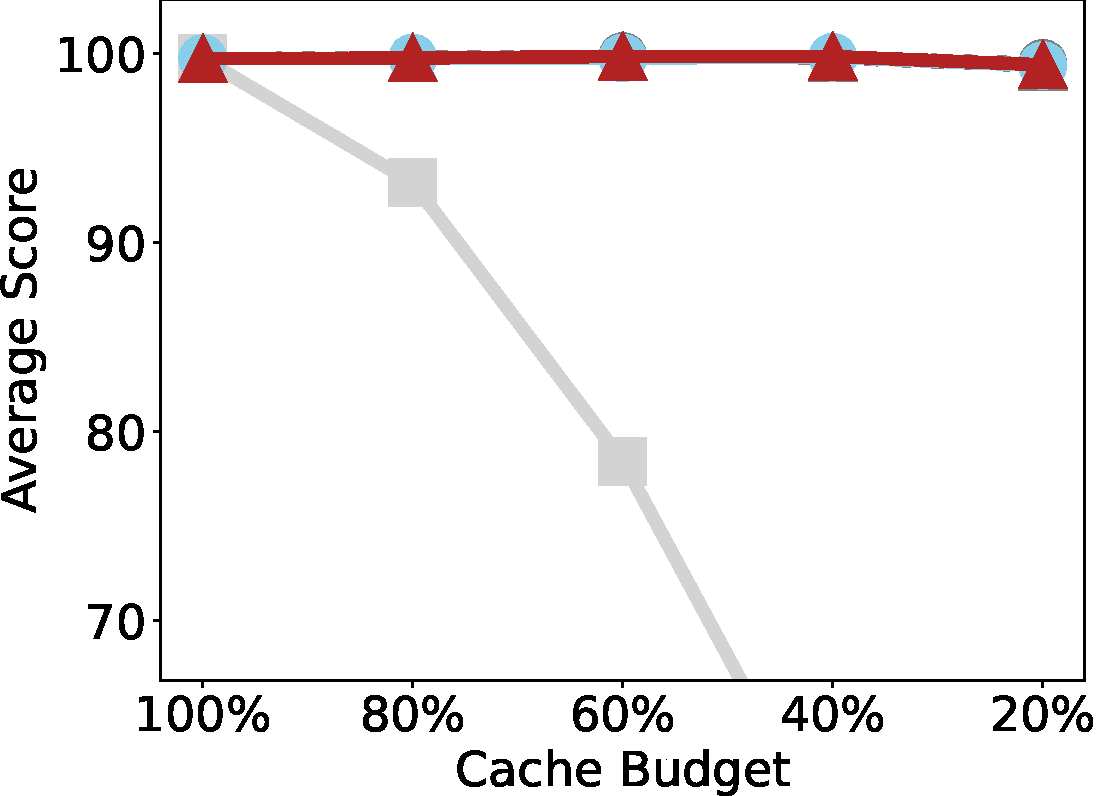
\includegraphics[width=\linewidth]{./Figures/ruler_per_dataset_group_by_wq/vt_wq_Llama3.1_ruler_score.pdf} 
		\caption{VT}
	\end{subfigure}
	\begin{subfigure}[b]{0.16\linewidth}
		\centering
		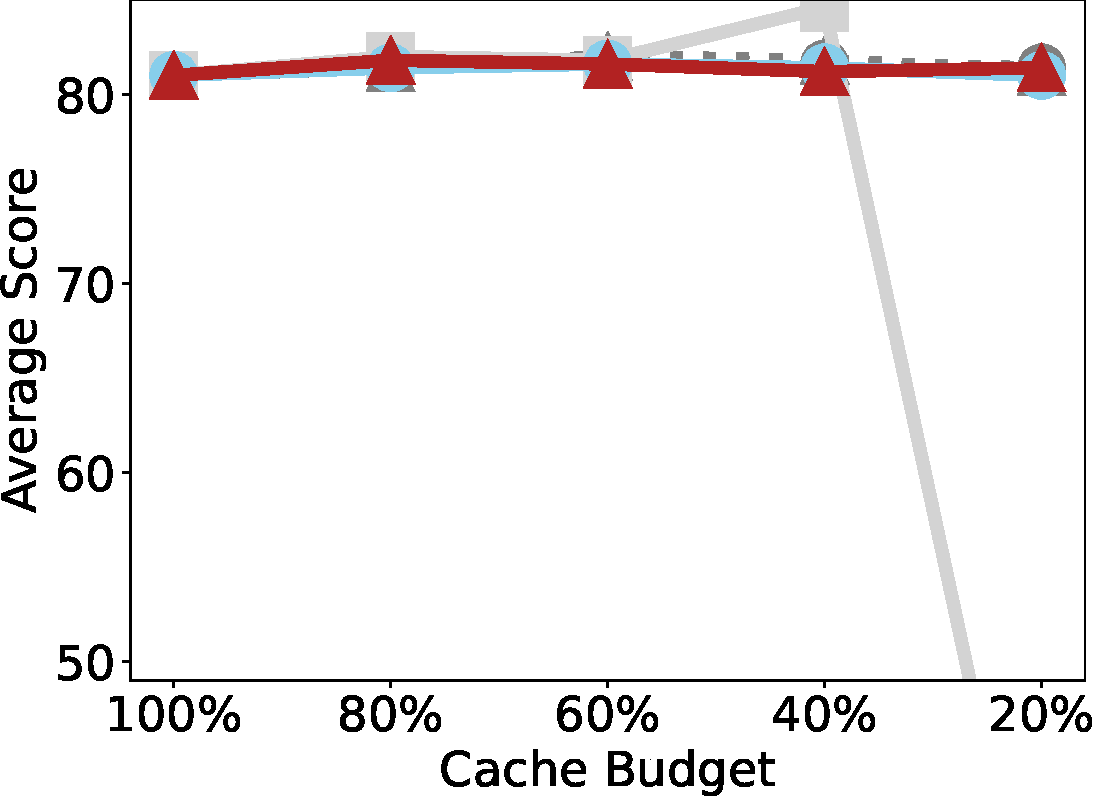
\includegraphics[width=\linewidth]{./Figures/ruler_per_dataset_group_by_wq/qa_1_wq_Llama3.1_ruler_score.pdf}
		\caption{S-QA}
	\end{subfigure}
		\begin{subfigure}[b]{0.16\linewidth}
		\centering
		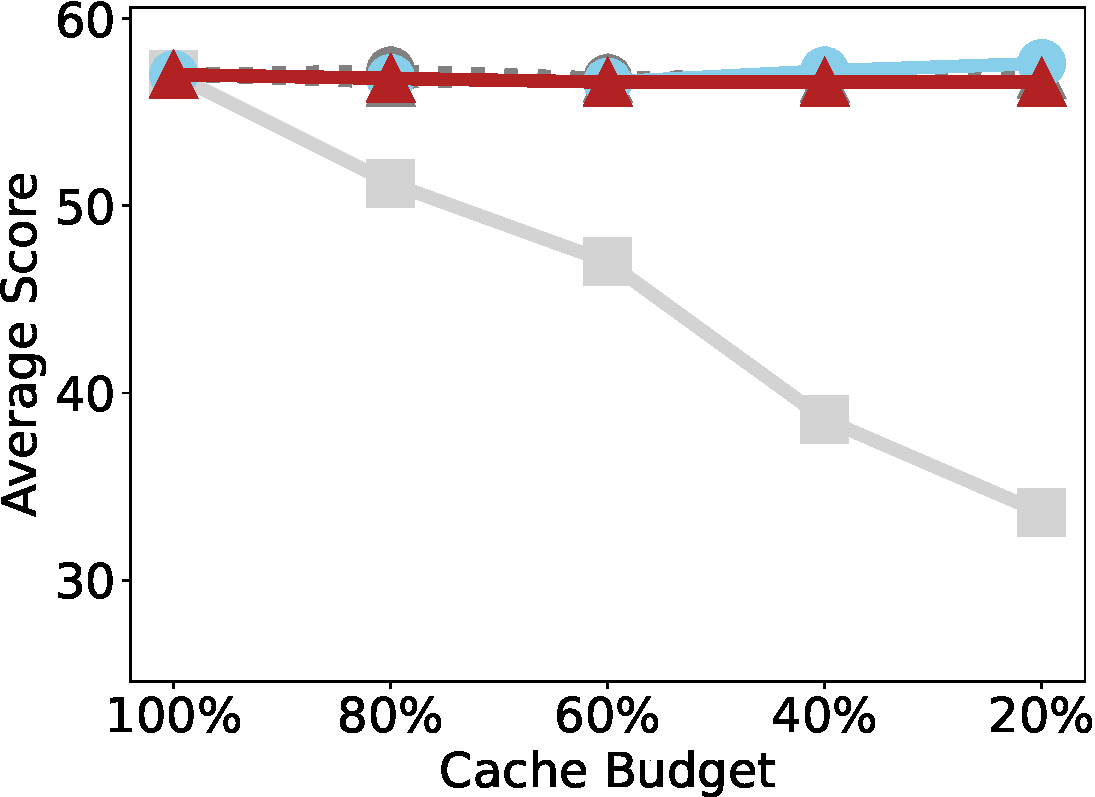
\includegraphics[width=\linewidth]{./Figures/ruler_per_dataset_group_by_wq/qa_2_wq_Llama3.1_ruler_score.pdf}
		\caption{M-QA}
	\end{subfigure}
    \caption{Subtask Analysis on Ruler (Question-aware, Llama3.1-8B-Instruct).}
	\label{fig:aware_llama_ruler_subtask}
\end{figure*}

\begin{figure*}[h!]
	\begin{minipage}{\linewidth}
		\centering
		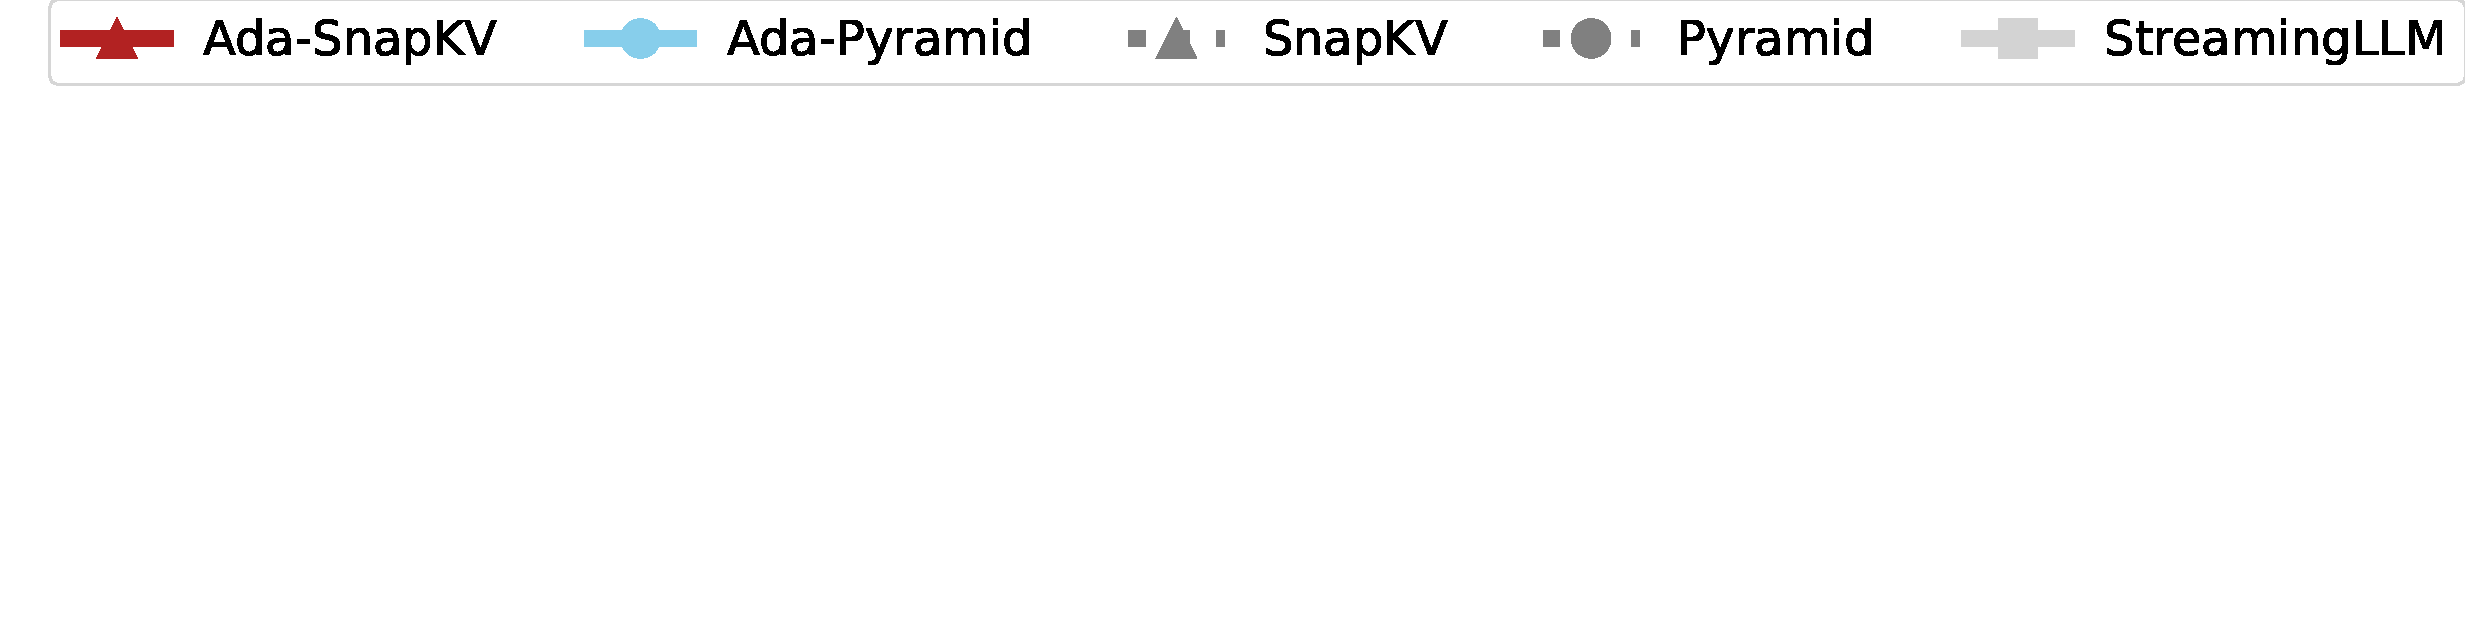
\includegraphics[width=0.7\linewidth]{./Figures/ruler_per_dataset_group_by_wq/legend.pdf} 
	\end{minipage}
	\begin{subfigure}[b]{0.16\linewidth}
		\centering
		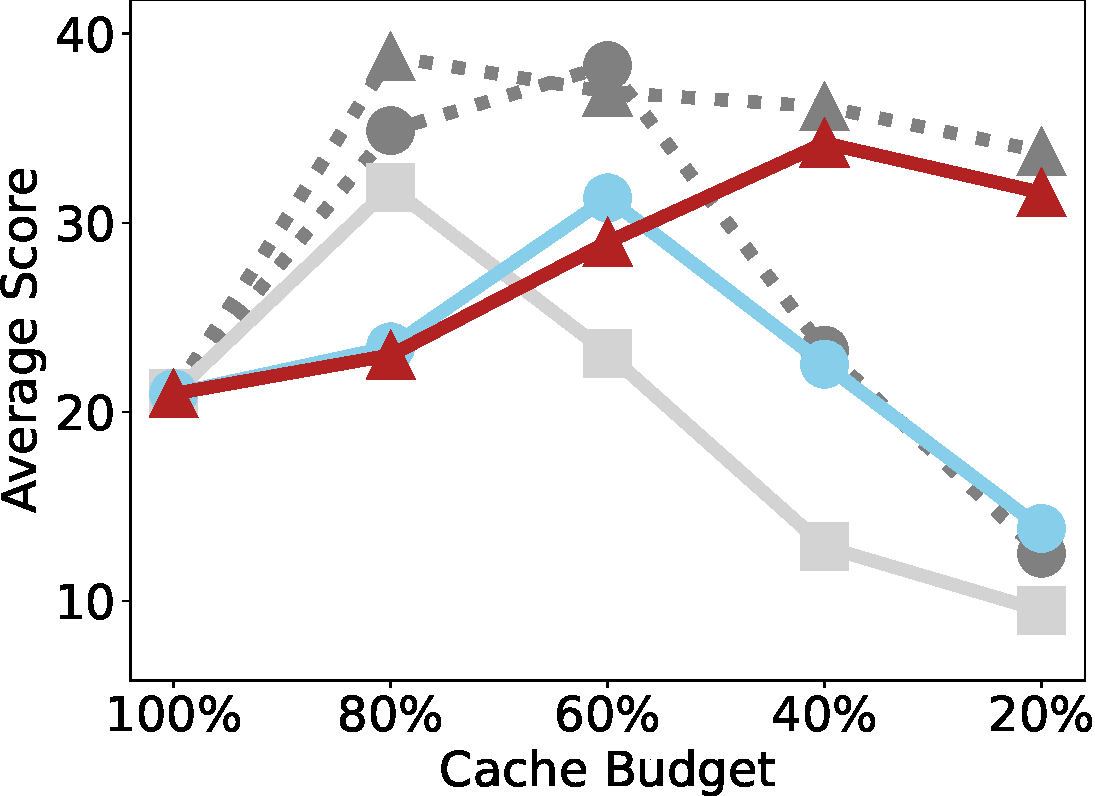
\includegraphics[width=\linewidth]{./Figures/ruler_per_dataset_group_by_wq/cwe_Mistral_ruler_score.pdf} 
		\caption{CWE}
	\end{subfigure}
	\begin{subfigure}[b]{0.16\linewidth}
		\centering
		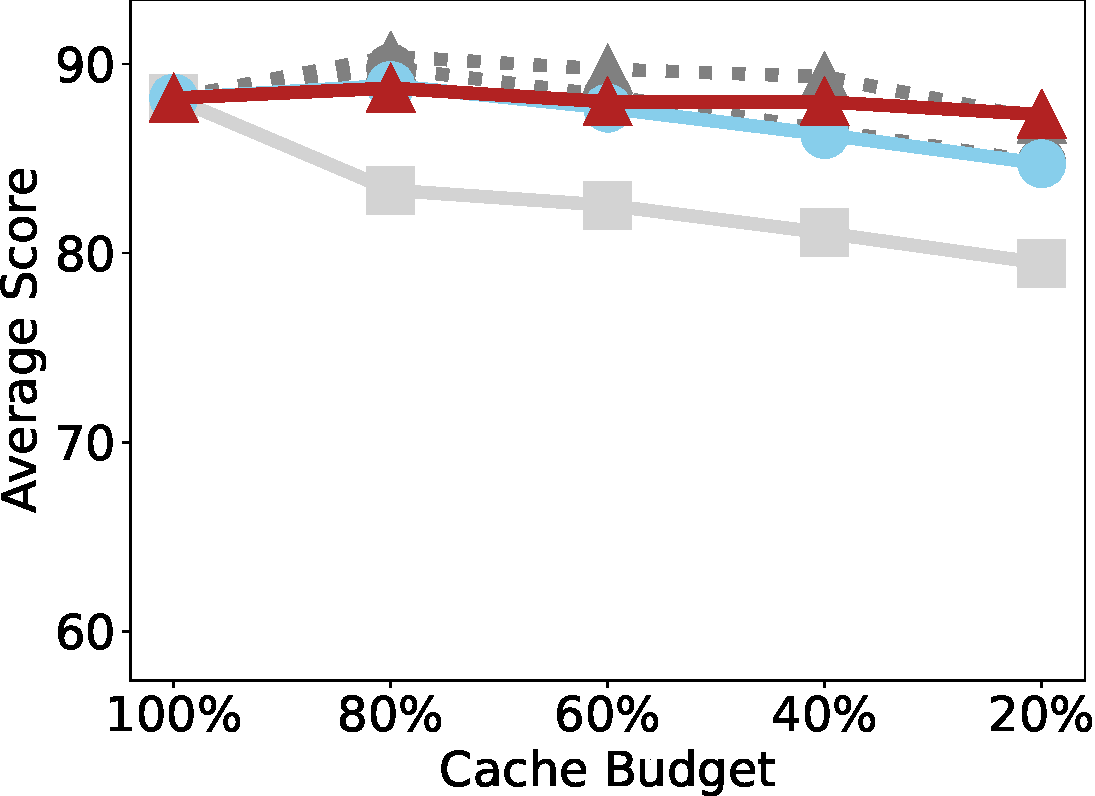
\includegraphics[width=\linewidth]{./Figures/ruler_per_dataset_group_by_wq/fwe_Mistral_ruler_score.pdf}
		\caption{FWE}
	\end{subfigure}
	\begin{subfigure}[b]{0.16\linewidth}
		\centering
		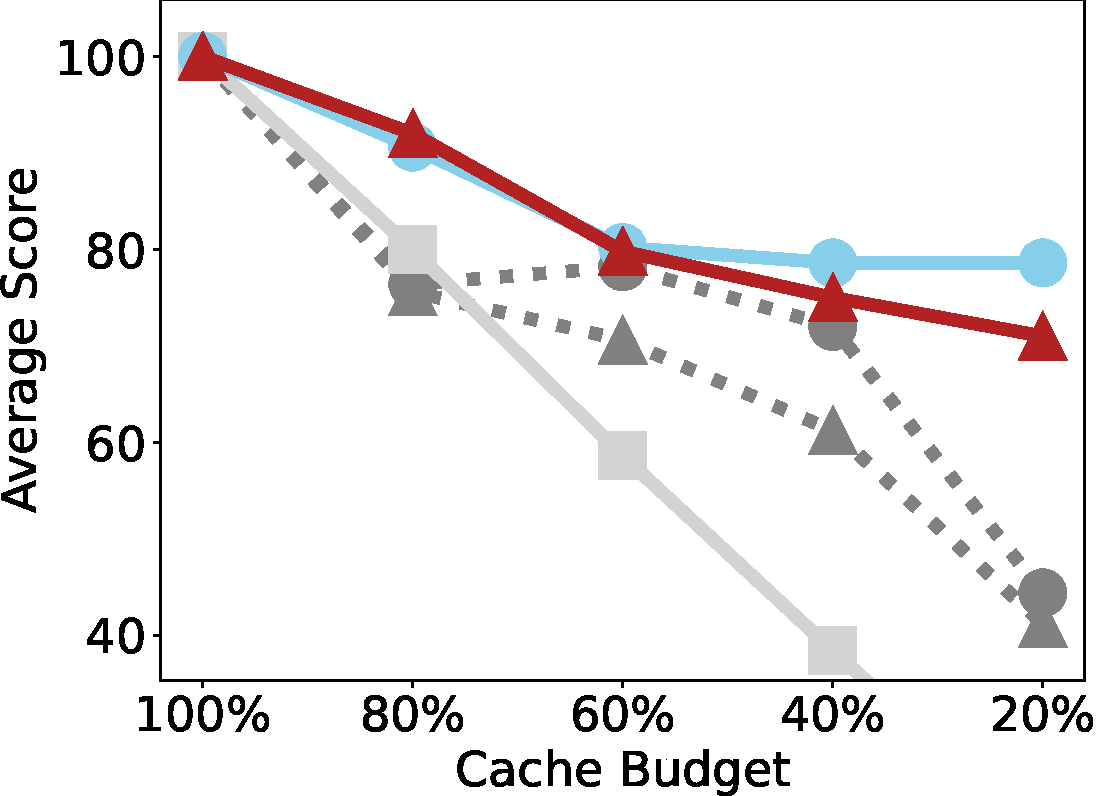
\includegraphics[width=\linewidth]{./Figures/ruler_per_dataset_group_by_wq/niah_single_1_Mistral_ruler_score.pdf} 
		\caption{S-NIAH-1}
	\end{subfigure}
	\begin{subfigure}[b]{0.16\linewidth}
		\centering
		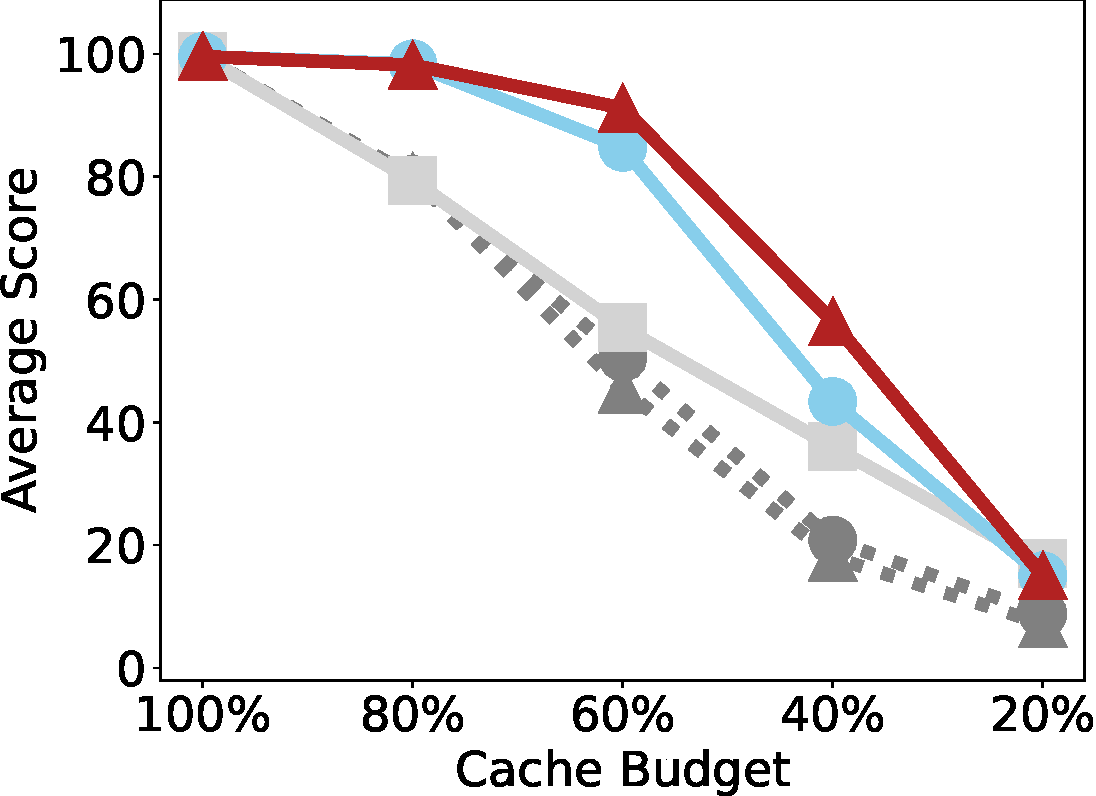
\includegraphics[width=\linewidth]{./Figures/ruler_per_dataset_group_by_wq/niah_single_2_Mistral_ruler_score.pdf}
		\caption{S-NIAH-2}
	\end{subfigure}
	\begin{subfigure}[b]{0.16\linewidth}
		\centering
		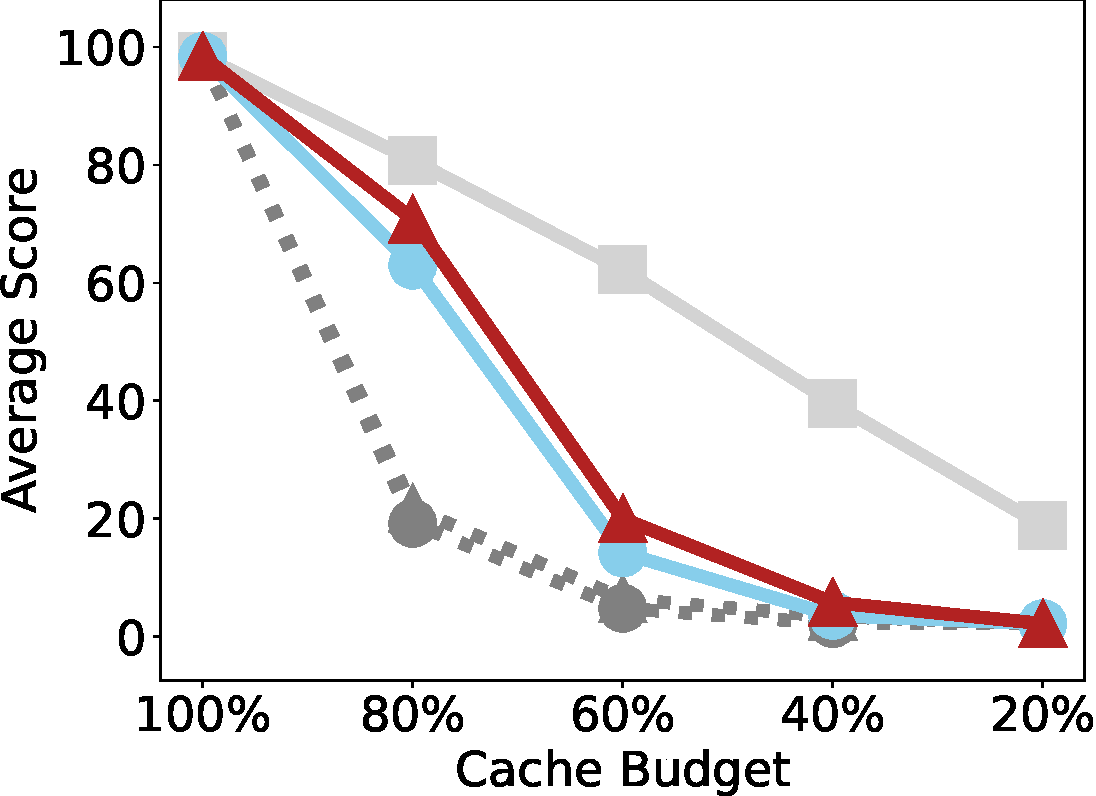
\includegraphics[width=\linewidth]{./Figures/ruler_per_dataset_group_by_wq/niah_single_3_Mistral_ruler_score.pdf} 
		\caption{S-NIAH-3}
	\end{subfigure}
	\begin{subfigure}[b]{0.16\linewidth}
		\centering
		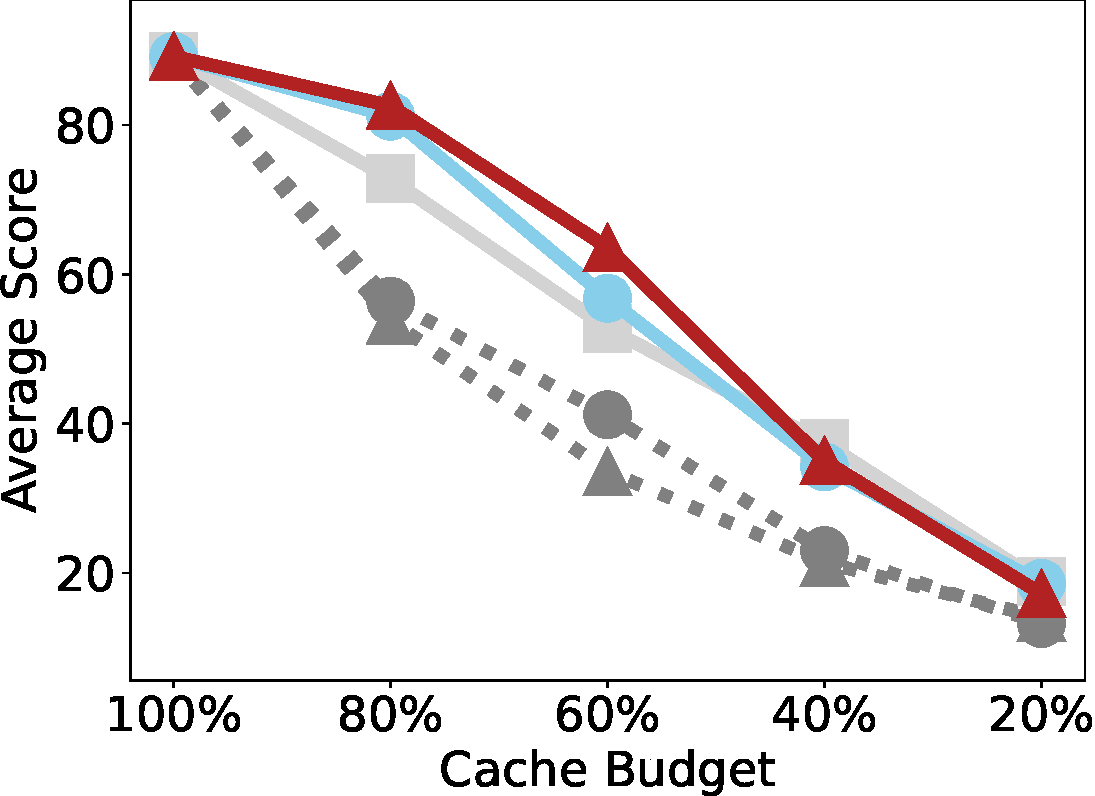
\includegraphics[width=\linewidth]{./Figures/ruler_per_dataset_group_by_wq/niah_multikey_1_Mistral_ruler_score.pdf}
		\caption{MK-NIAH-1}
	\end{subfigure}
	\begin{subfigure}[b]{0.16\linewidth}
		\centering
		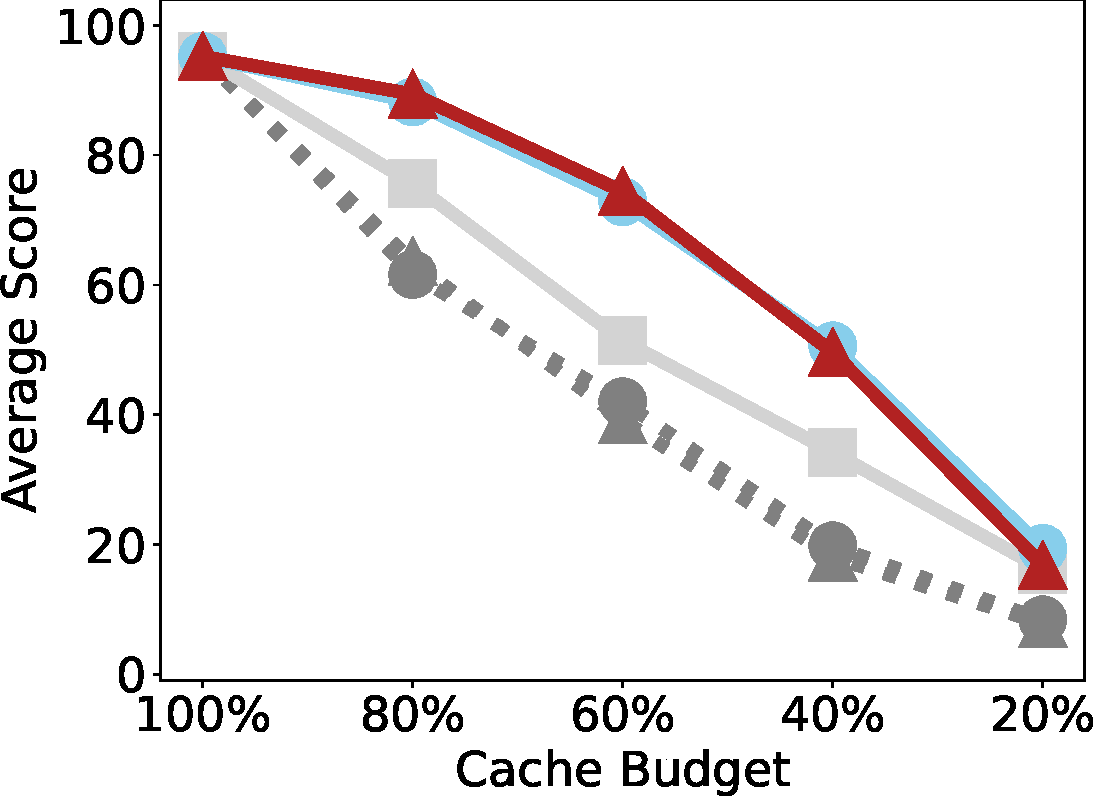
\includegraphics[width=\linewidth]{./Figures/ruler_per_dataset_group_by_wq/niah_multikey_2_Mistral_ruler_score.pdf} 
		\caption{MK-NIAH-2}
	\end{subfigure}
	\begin{subfigure}[b]{0.16\linewidth}
		\centering
		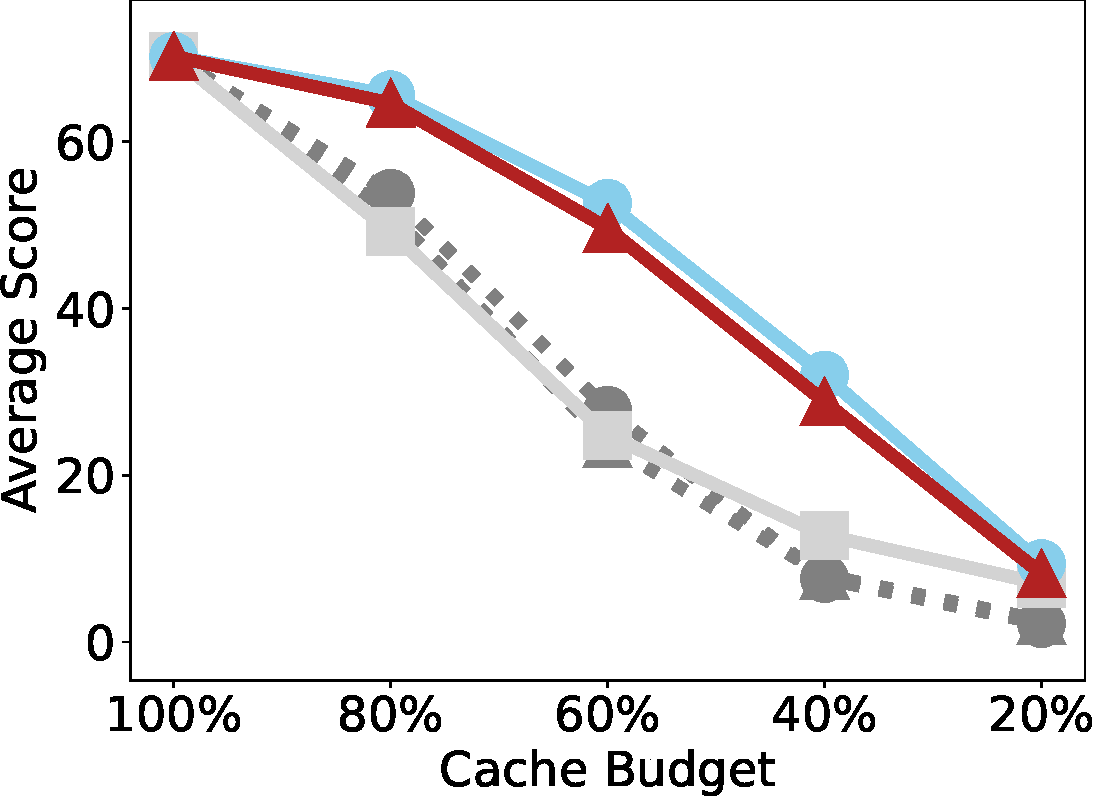
\includegraphics[width=\linewidth]{./Figures/ruler_per_dataset_group_by_wq/niah_multikey_3_Mistral_ruler_score.pdf}
		\caption{MK-NIAH-3}
	\end{subfigure}
	\begin{subfigure}[b]{0.16\linewidth}
		\centering
		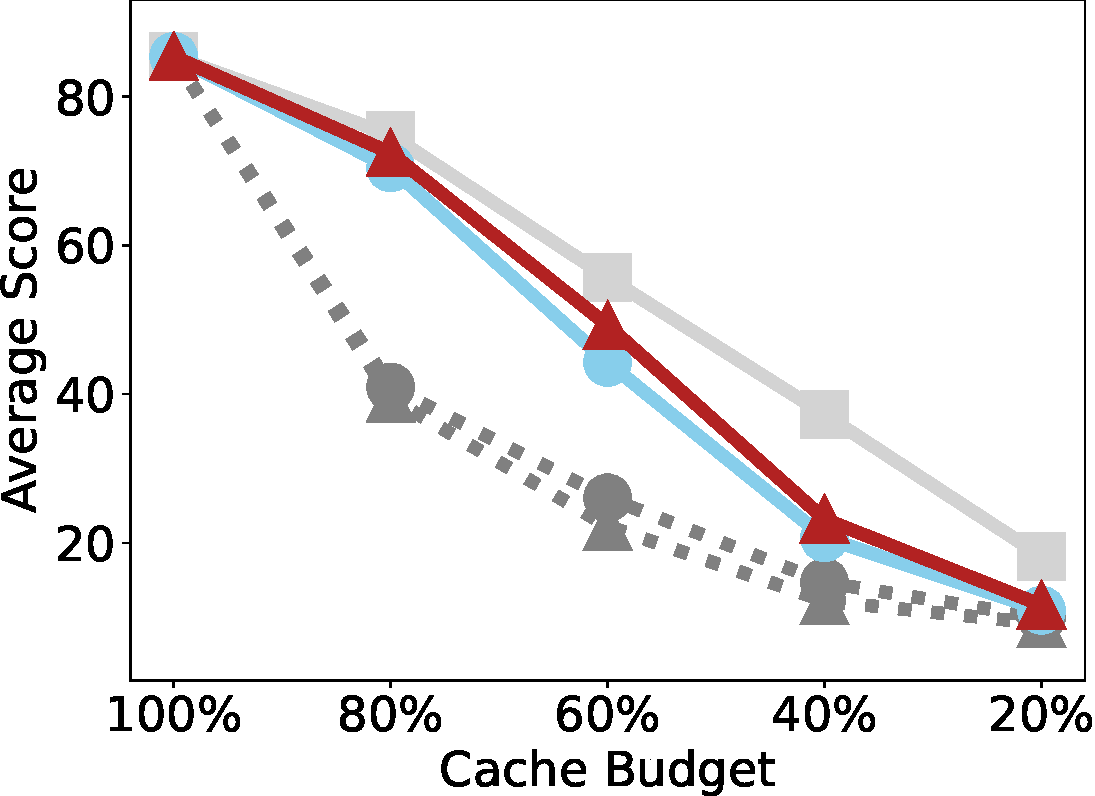
\includegraphics[width=\linewidth]{./Figures/ruler_per_dataset_group_by_wq/niah_multivalue_Mistral_ruler_score.pdf}
		\caption{MV-NIAH}
	\end{subfigure}
	\begin{subfigure}[b]{0.16\linewidth}
		\centering
		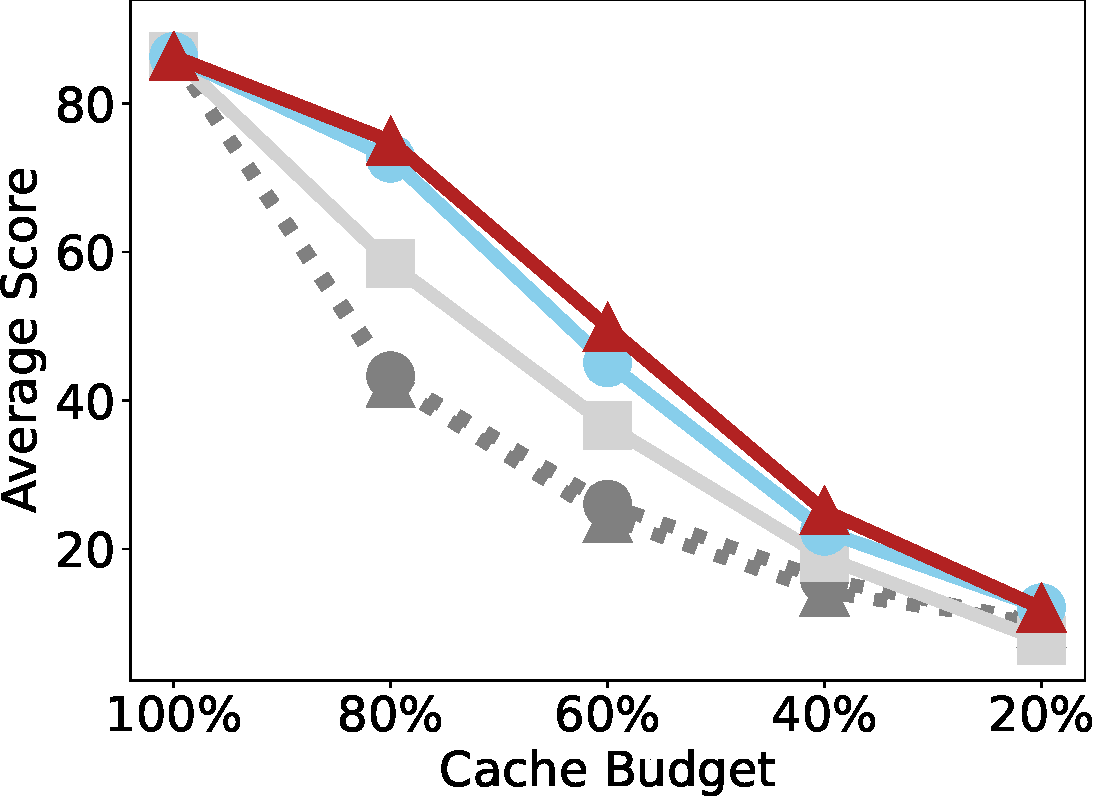
\includegraphics[width=\linewidth]{./Figures/ruler_per_dataset_group_by_wq/niah_multiquery_Mistral_ruler_score.pdf}
		\caption{MQ-NIAH}
	\end{subfigure}
	\begin{subfigure}[b]{0.16\linewidth}
		\centering
		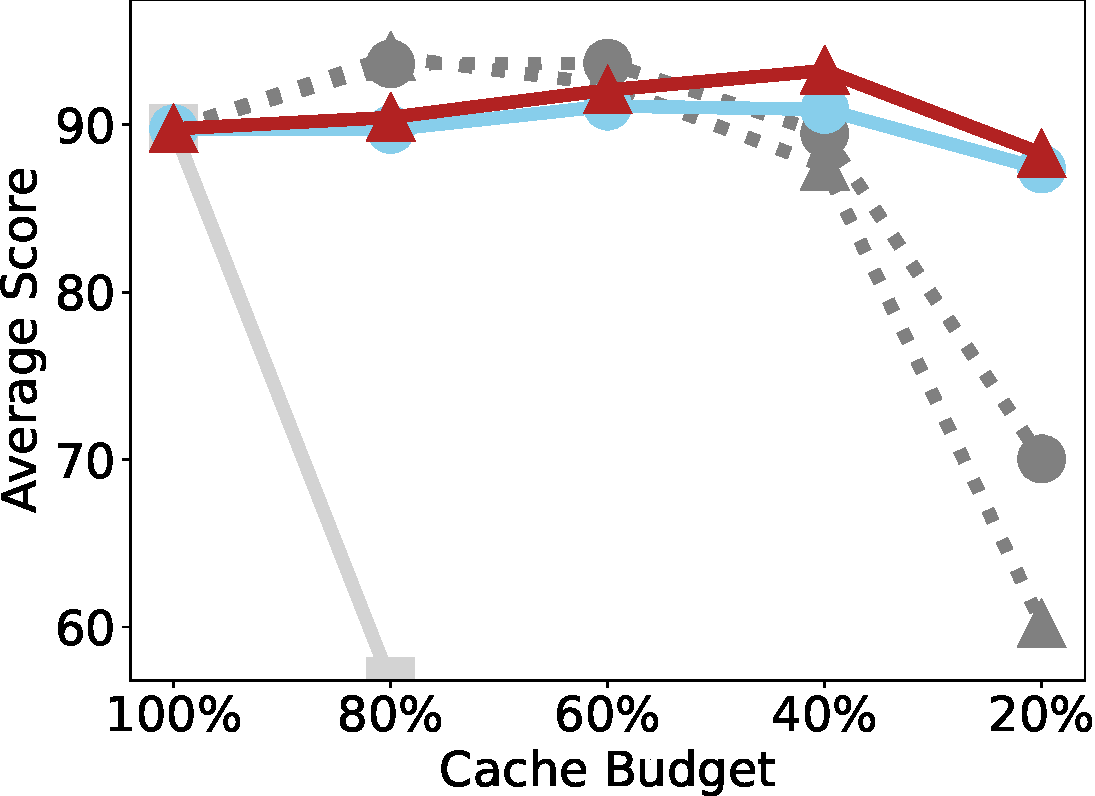
\includegraphics[width=\linewidth]{./Figures/ruler_per_dataset_group_by_wq/vt_Mistral_ruler_score.pdf} 
		\caption{VT}
	\end{subfigure}
	\begin{subfigure}[b]{0.16\linewidth}
		\centering
		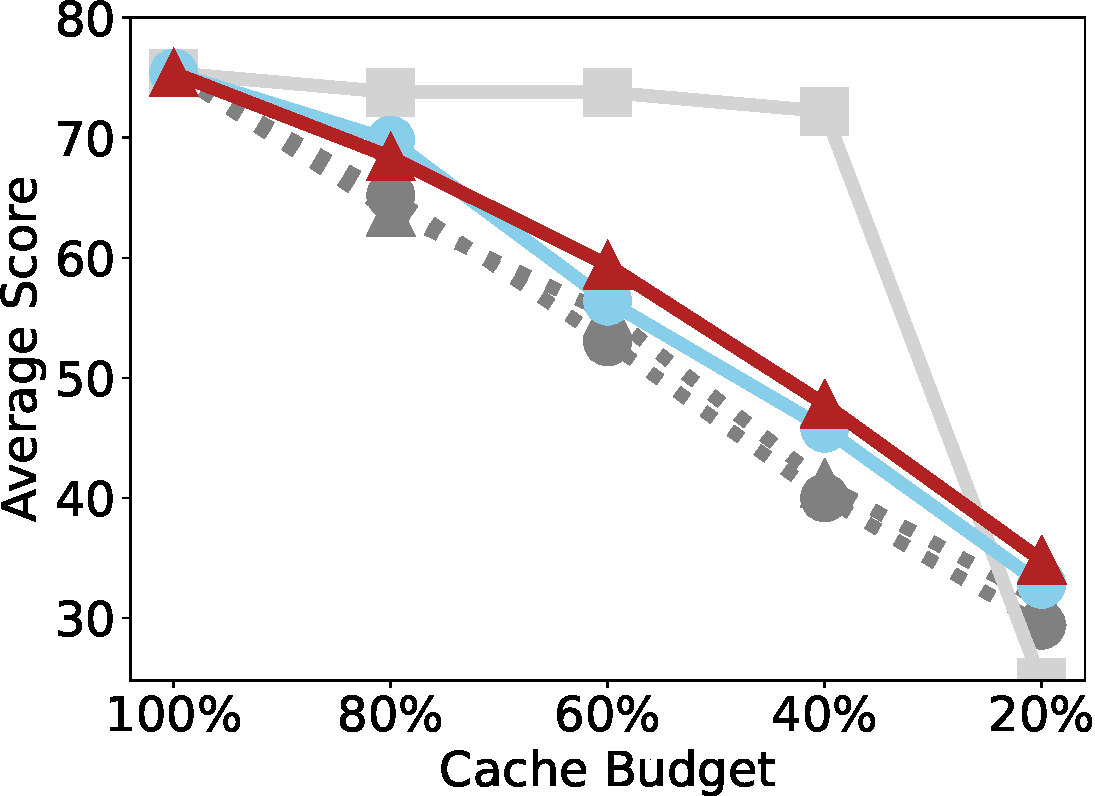
\includegraphics[width=\linewidth]{./Figures/ruler_per_dataset_group_by_wq/qa_1_Mistral_ruler_score.pdf}
		\caption{S-QA}
	\end{subfigure}
	\begin{subfigure}[b]{0.16\linewidth}
		\centering
		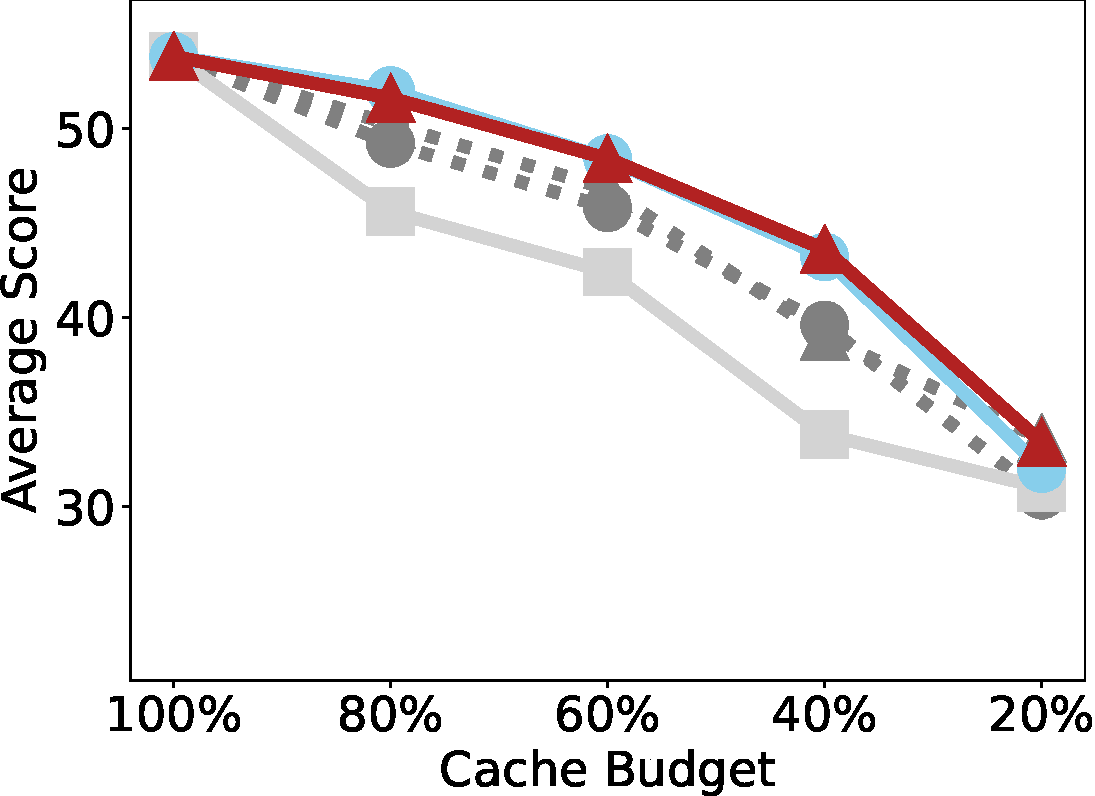
\includegraphics[width=\linewidth]{./Figures/ruler_per_dataset_group_by_wq/qa_2_Mistral_ruler_score.pdf}
		\caption{M-QA}
	\end{subfigure}
    \caption{Subtask Analysis on  Ruler (Question-agnostic, Mistral-7B-Instruct-v0.2).}
	\label{fig:agnostic_mistral_ruler_subtask}
\end{figure*}


\begin{figure*}[h!]
	\begin{minipage}{\linewidth}
	\centering
	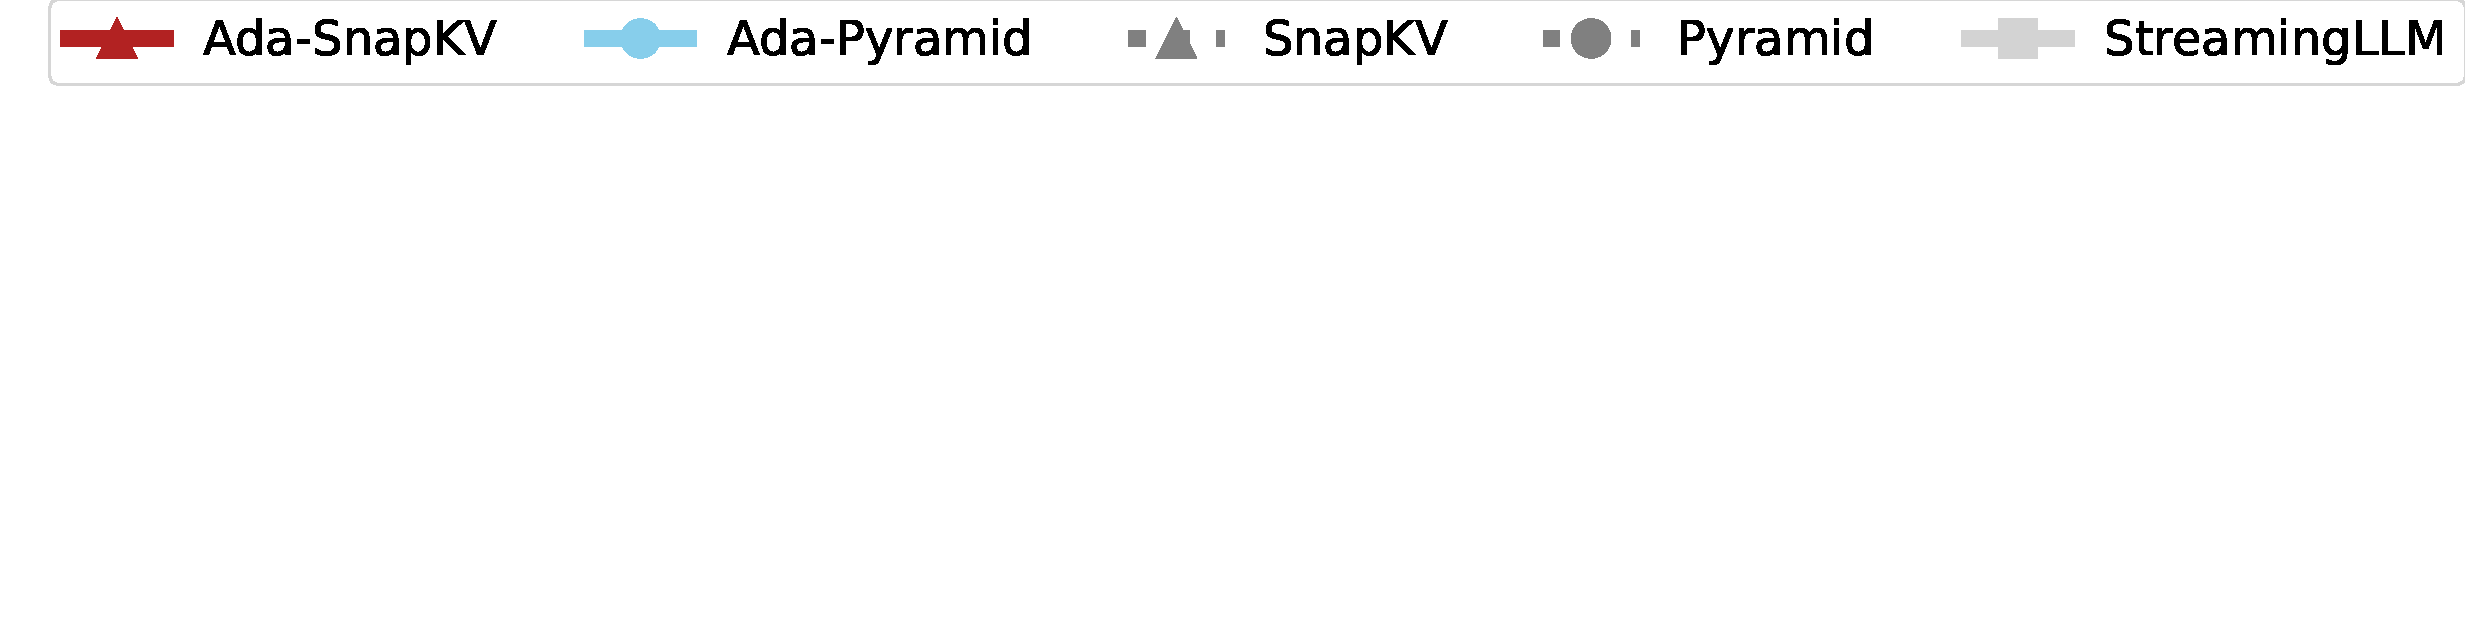
\includegraphics[width=0.7\linewidth]{./Figures/ruler_per_dataset_group_by_wq/legend.pdf} 
	\end{minipage}
	\begin{subfigure}[b]{0.16\linewidth}
		\centering
		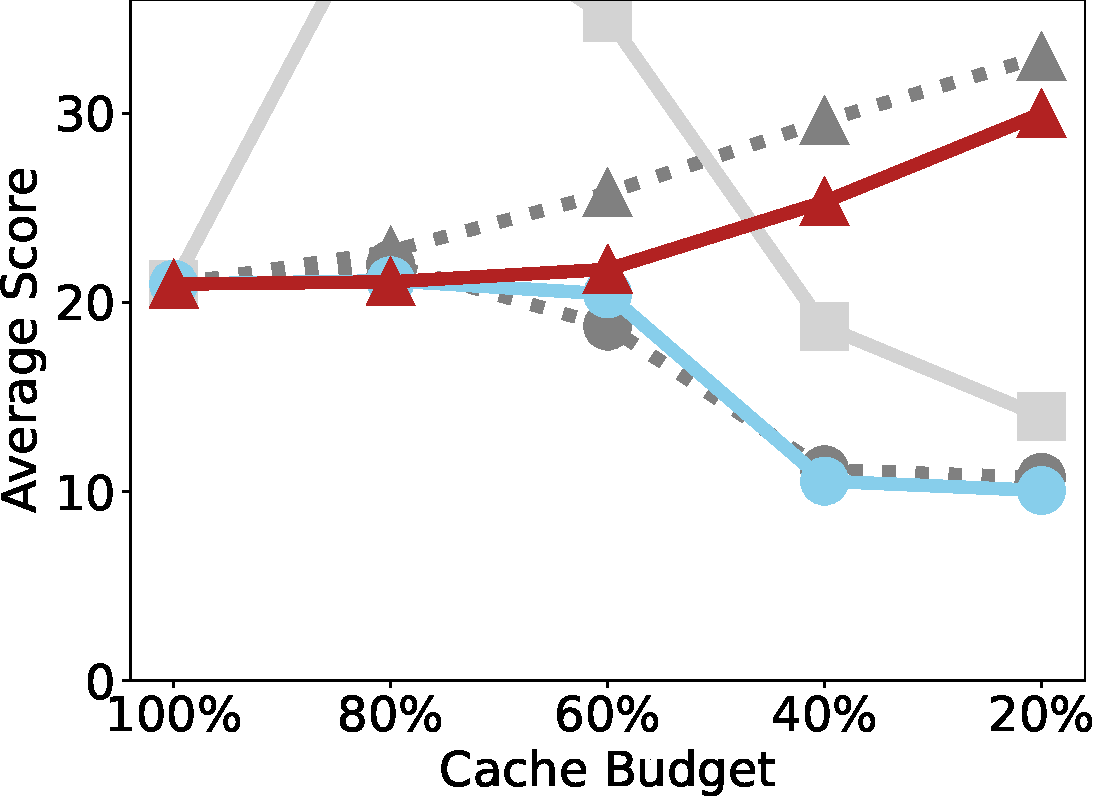
\includegraphics[width=\linewidth]{./Figures/ruler_per_dataset_group_by_wq/cwe_wq_Mistral_ruler_score.pdf} 
		\caption{CWE}
	\end{subfigure}
	\begin{subfigure}[b]{0.16\linewidth}
		\centering
		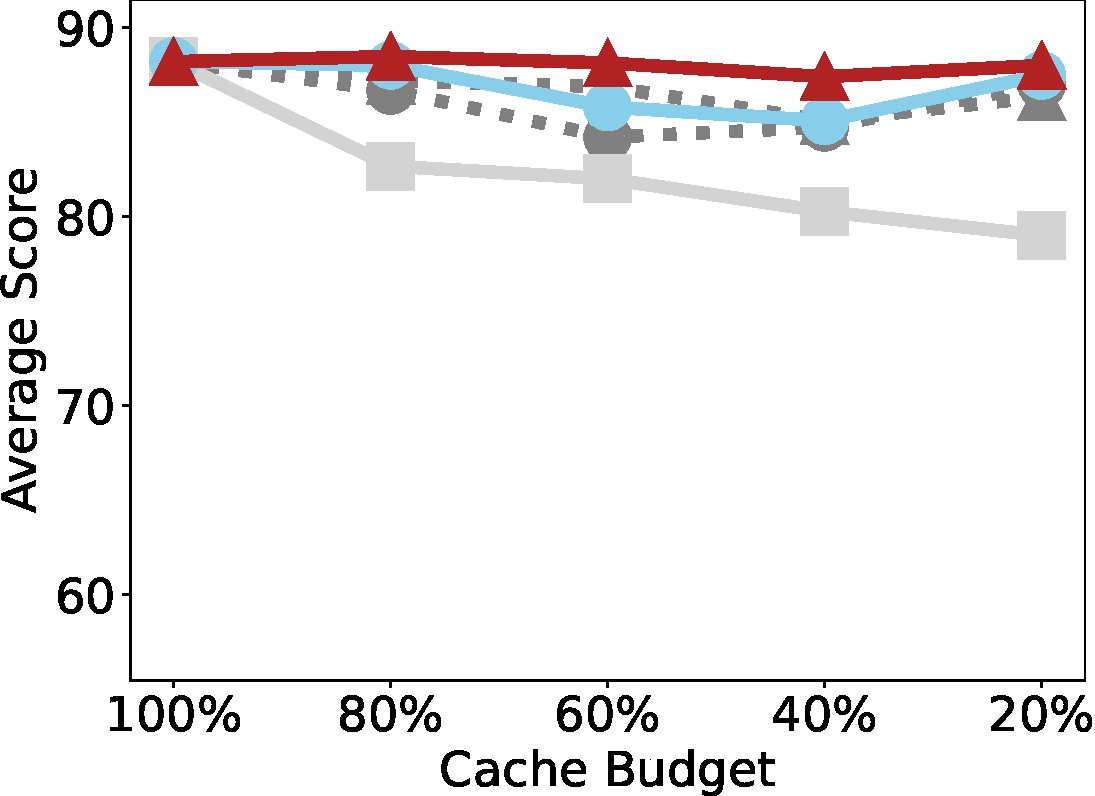
\includegraphics[width=\linewidth]{./Figures/ruler_per_dataset_group_by_wq/fwe_wq_Mistral_ruler_score.pdf}
		\caption{FWE}
	\end{subfigure}
	\begin{subfigure}[b]{0.16\linewidth}
		\centering
		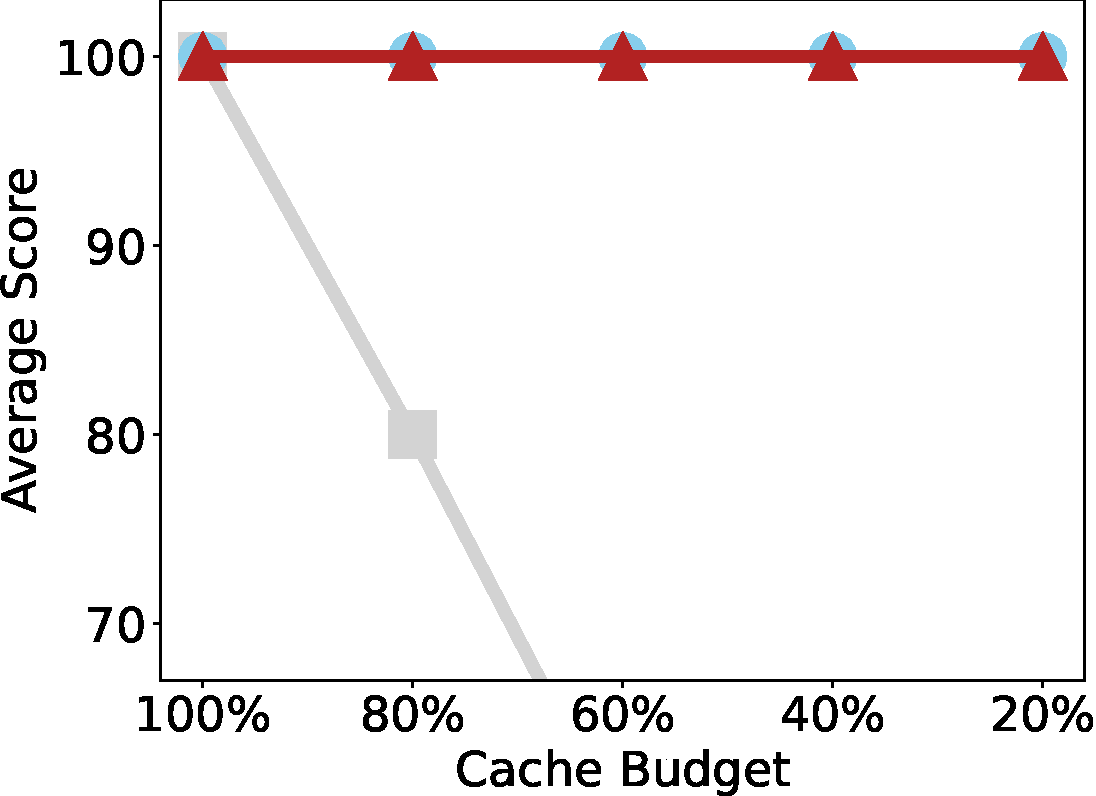
\includegraphics[width=\linewidth]{./Figures/ruler_per_dataset_group_by_wq/niah_single_1_wq_Mistral_ruler_score.pdf} 
		\caption{S-NIAH-1}
	\end{subfigure}
	\begin{subfigure}[b]{0.16\linewidth}
		\centering
		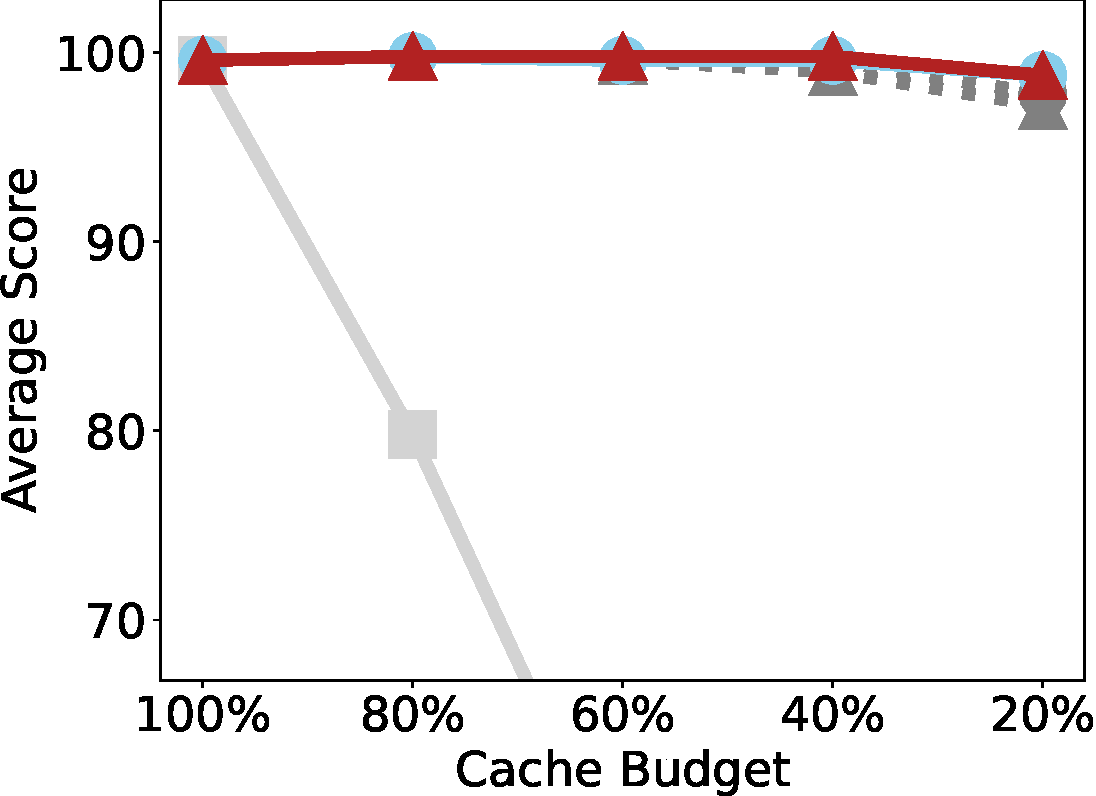
\includegraphics[width=\linewidth]{./Figures/ruler_per_dataset_group_by_wq/niah_single_2_wq_Mistral_ruler_score.pdf}
		\caption{S-NIAH-2}
	\end{subfigure}
	\begin{subfigure}[b]{0.16\linewidth}
		\centering
		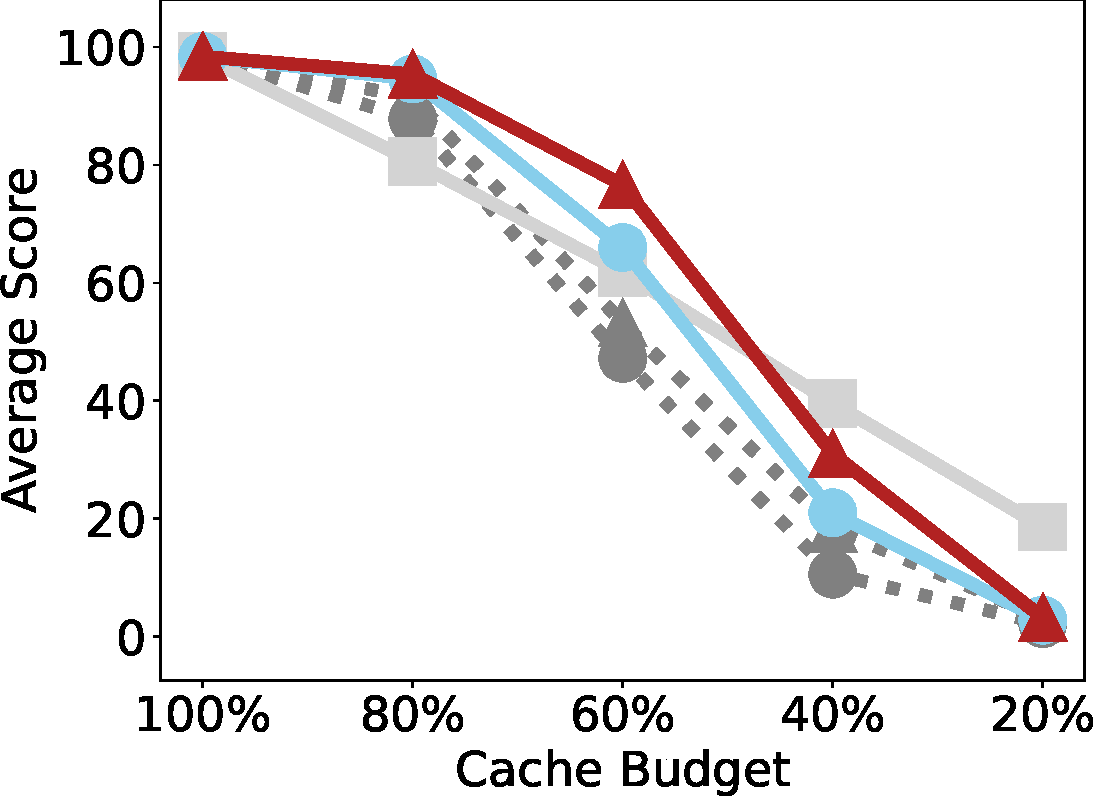
\includegraphics[width=\linewidth]{./Figures/ruler_per_dataset_group_by_wq/niah_single_3_wq_Mistral_ruler_score.pdf} 
		\caption{S-NIAH-3}
	\end{subfigure}
	\begin{subfigure}[b]{0.16\linewidth}
		\centering
		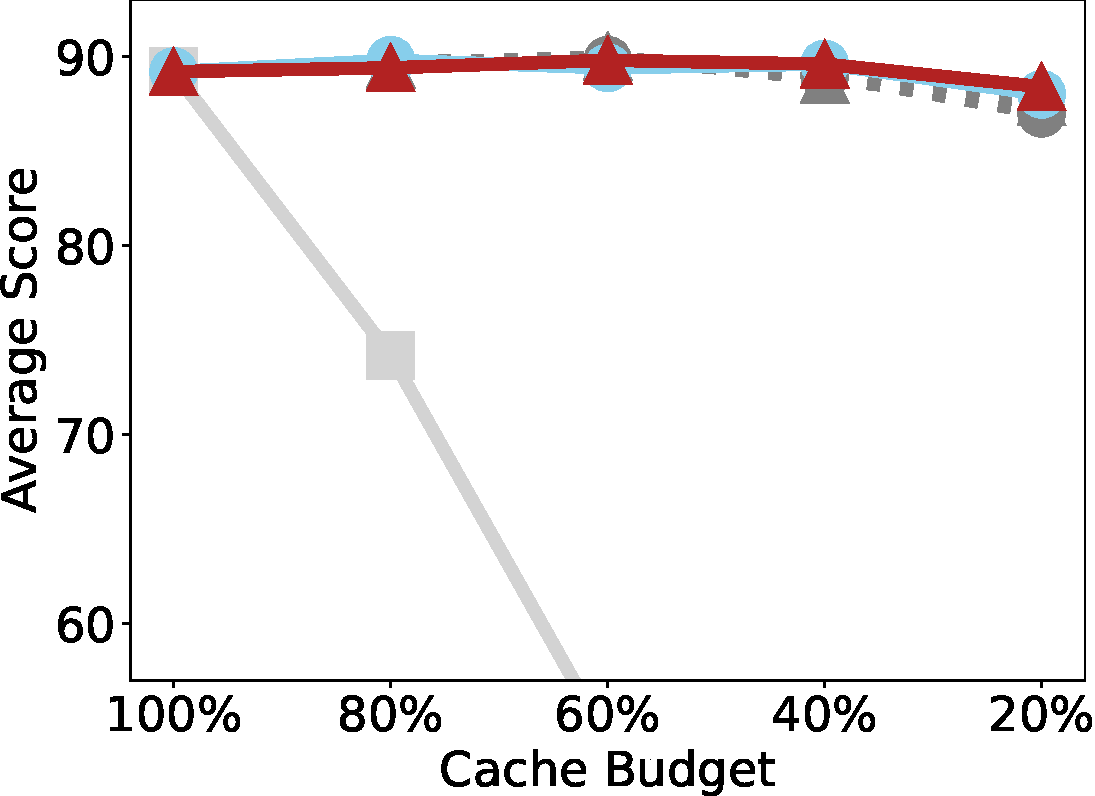
\includegraphics[width=\linewidth]{./Figures/ruler_per_dataset_group_by_wq/niah_multikey_1_wq_Mistral_ruler_score.pdf}
		\caption{MK-NIAH-1}
	\end{subfigure}
	\begin{subfigure}[b]{0.16\linewidth}
		\centering
		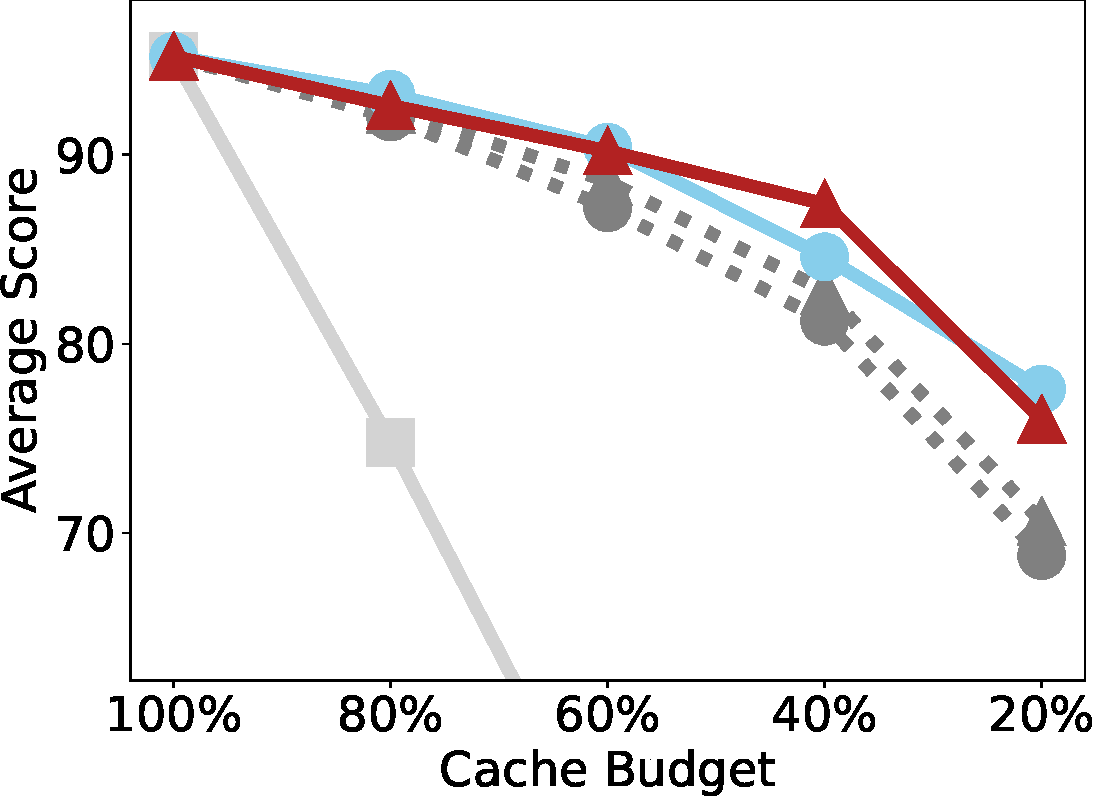
\includegraphics[width=\linewidth]{./Figures/ruler_per_dataset_group_by_wq/niah_multikey_2_wq_Mistral_ruler_score.pdf} 
		\caption{MK-NIAH-2}
	\end{subfigure}
	\begin{subfigure}[b]{0.16\linewidth}
		\centering
		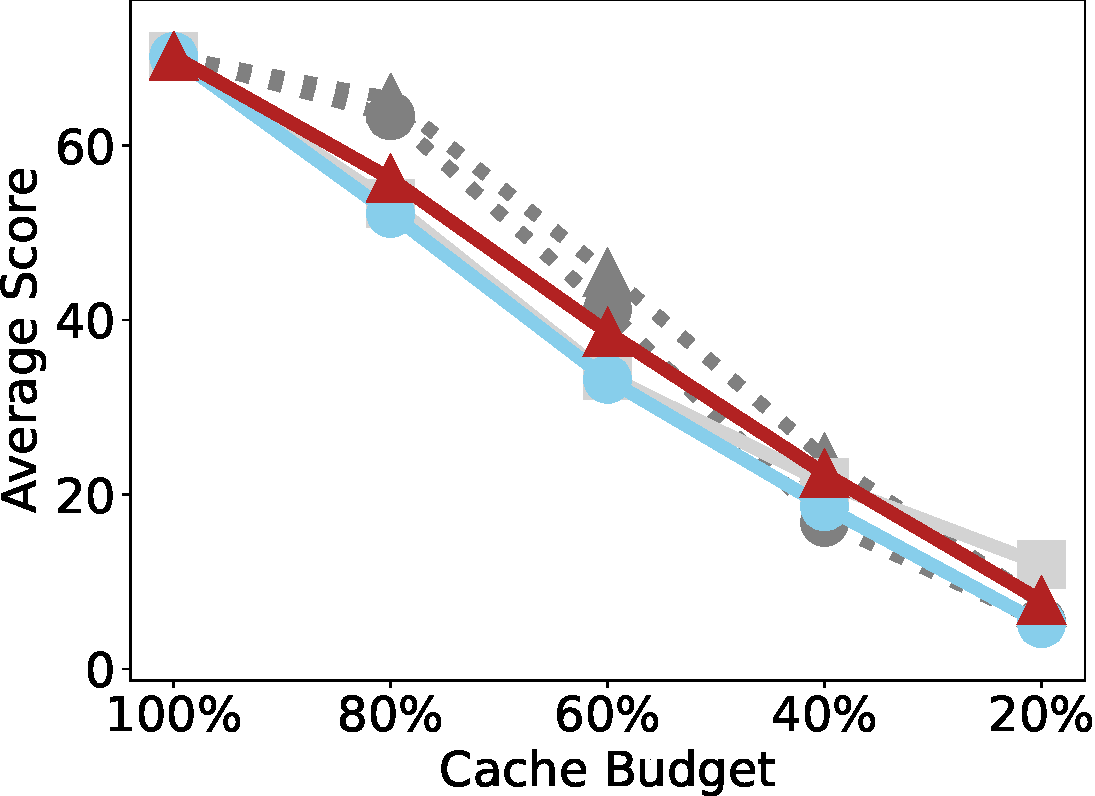
\includegraphics[width=\linewidth]{./Figures/ruler_per_dataset_group_by_wq/niah_multikey_3_wq_Mistral_ruler_score.pdf}
		\caption{MK-NIAH-3}
	\end{subfigure}
	\begin{subfigure}[b]{0.16\linewidth}
		\centering
		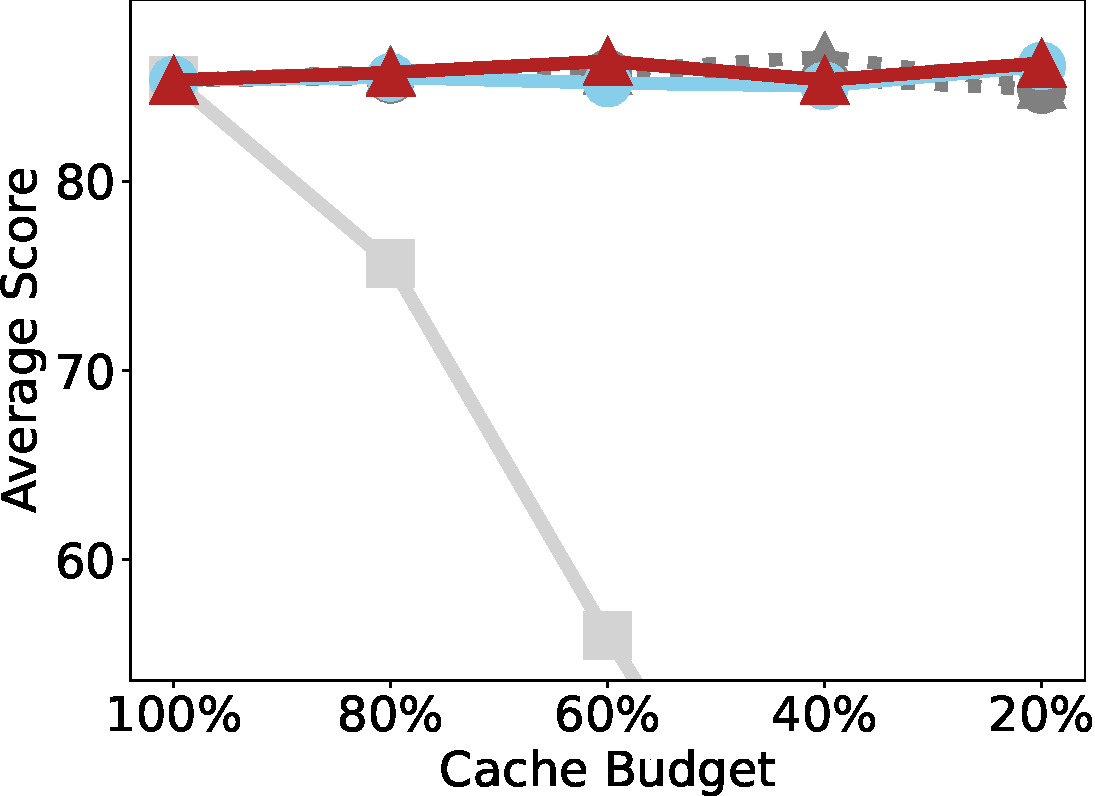
\includegraphics[width=\linewidth]{./Figures/ruler_per_dataset_group_by_wq/niah_multivalue_wq_Mistral_ruler_score.pdf}
		\caption{MV-NIAH}
	\end{subfigure}
	\begin{subfigure}[b]{0.16\linewidth}
		\centering
		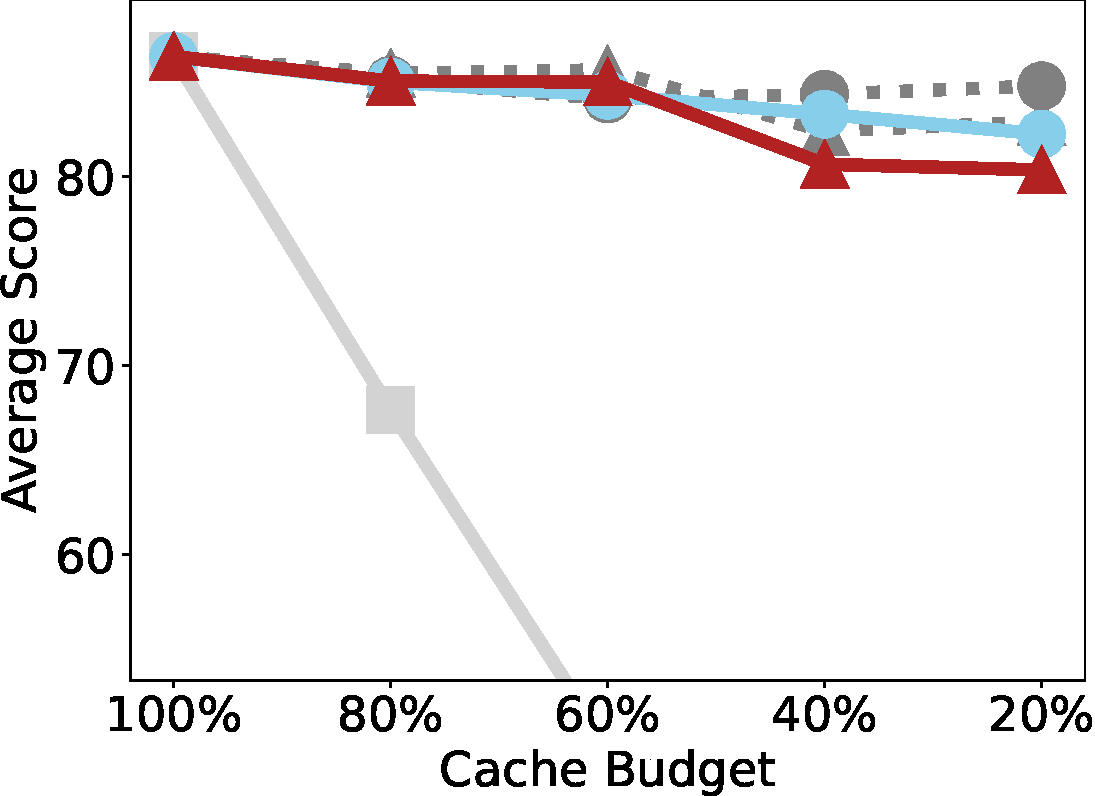
\includegraphics[width=\linewidth]{./Figures/ruler_per_dataset_group_by_wq/niah_multiquery_wq_Mistral_ruler_score.pdf}
		\caption{MQ-NIAH}
	\end{subfigure}
	\begin{subfigure}[b]{0.16\linewidth}
		\centering
		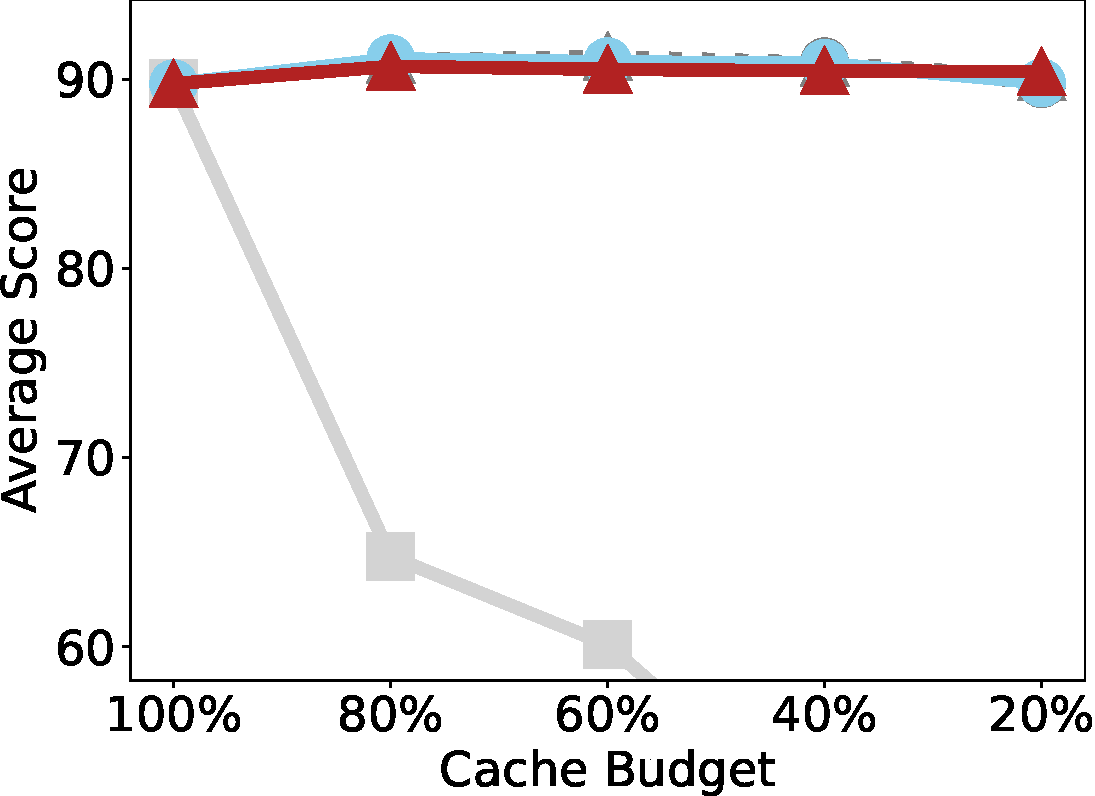
\includegraphics[width=\linewidth]{./Figures/ruler_per_dataset_group_by_wq/vt_wq_Mistral_ruler_score.pdf} 
		\caption{VT}
	\end{subfigure}
	\begin{subfigure}[b]{0.16\linewidth}
		\centering
		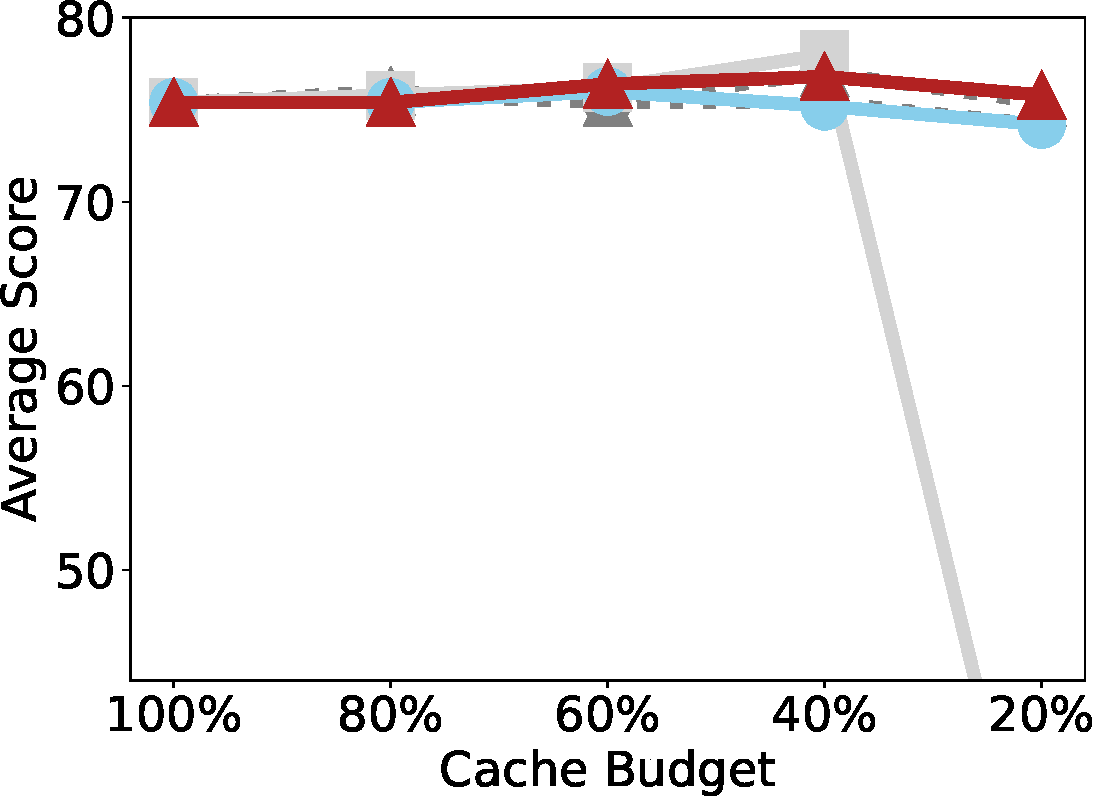
\includegraphics[width=\linewidth]{./Figures/ruler_per_dataset_group_by_wq/qa_1_wq_Mistral_ruler_score.pdf}
		\caption{S-QA}
	\end{subfigure}
		\begin{subfigure}[b]{0.16\linewidth}
		\centering
		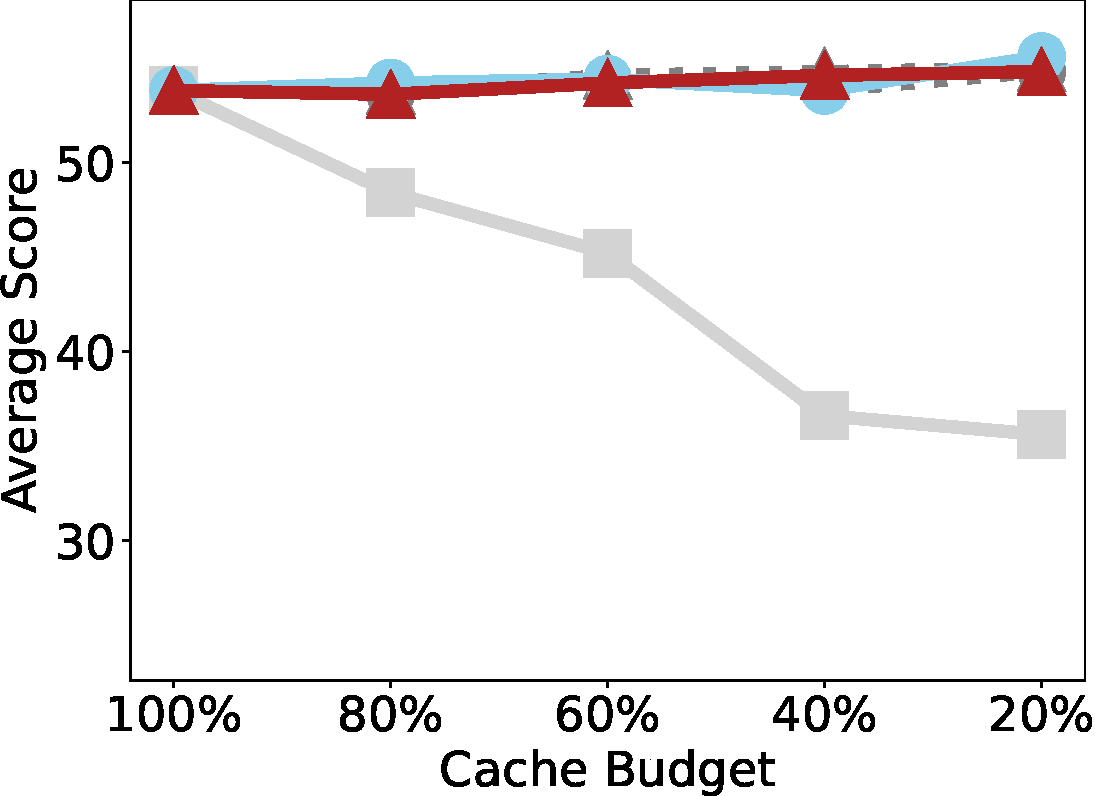
\includegraphics[width=\linewidth]{./Figures/ruler_per_dataset_group_by_wq/qa_2_wq_Mistral_ruler_score.pdf}
		\caption{M-QA}
	\end{subfigure}
    \caption{Subtask Analysis on Ruler (Question-aware, Mistral-7B-Instruct-v0.2).}
	\label{fig:aware_mistral_ruler_subtask}
\end{figure*}




\subsection{Detail results of LongBench Evaluation}
\label{apdx:detail_LongBench}
Tables \ref{tbl:detailed_llama_longbench}, \ref{tbl:detailed_mistral_longbench}, \ref{tbl:detailed_mistral_longbench_question_agnostic} and \ref{tbl:detailed_llama_longbench_question_agnostic} present the detailed evaluation results of different methods across 16 datasets on LongBench for two models. As shown, the Ada-SnapKV and Ada-Pyramid methods, with our adaptive allocation enhancement, achieve consistent improvements in overall generation quality across different budgets and models.




\subsection{Detailed Information of Ruler Benchmark}
\label{apdx:ruler_info}


Below is a brief overview of the different tasks in Ruler. For detailed examples, please refer to Tables \ref{tab:ruler_task_template1} \ref{tab:ruler_task_template2} and \ref{tab:ruler_task_template3}.   We adhere to the input prompt format from KVPress \cite{kvpress}, dividing the input into context and question segments. The question segment is highlighted in green, while other colors represent the context segment. In question-aware compression, both the context and question segments are input into the model and compressed. For question-agnostic compression, where future questions are unpredictable, only the context segment is input for compression. After compression, the question segment is input for answer generation.

\begin{itemize}
	\itemsep0em
	
	\item \textbf{Single NIAH (S-NIAH): } A basic information retrieval task. In this scenario, a keyword sentence, referred to as the "needle," is embedded within a lengthy text, called the "haystack." The goal is to retrieve the "needle" from the context. The "haystack" may consist of repetitive, noisy sentences or essays by Paul Graham~\cite{needle}.
	
	
	\item \textbf{Multi-keys NIAH (MK-NIAH): } Multiple "needles" are inserted into the "haystack," but the task requires retrieving only one of them.
	
	
	
	\item \textbf{Multi-values NIAH (MV-NIAH): } Multiple "needles" in the form of key-value pairs are placed within the "haystack." The task is to retrieve all values associated with a given key.
	
	
	\item \textbf{Multi-queries NIAH (MQ-NIAH): } Multiple "needle" in the form of key-value pairs are inserted into the "haystack". All "needles" corresponding to the keys specified in the queries need to be retrieved. ~\citet{mqar}
	
	
	
	\item \textbf{Variable Tracking (VT): } A series of variable binding statements (e.g., $X2 = X1, X3 = X2, ...$) are inserted at various positions within a long text to simulate the recognition of entities and relationships. The task objective is to return all variable names that point to the same value $V$.
	
	\item \textbf{Common words extraction task (CWE): } The input sequence is constructed by sampling words from a discrete uniform distribution within a pre-defined (synthetic) word list. Words that appear most frequently are termed "common words". The model is required to identify all common words. The number of common words remains constant while the number of uncommon words increases with the length of the sequence.
	
	
	
	\item \textbf{Frequent words extraction task (FWE): } The input sequence is constructed by sampling words from a Zeta distribution within a pre-defined (synthetic) word list. The model need to return the top-K frequent words in the context.
	
	\item \textbf{Single-Hop QA (S-QA)} Answer questions based on passages. The context is extended to simulate long-context input by adding distracting information(golden paragraphs). And answers come from a single piece of evidence.
	
	\item \textbf{Multi-Hop QA (M-QA)} Answer questions based on passages. For Multi-hop QA, which requires integrating information from multiple sources.
	
\end{itemize}

\subsection{Limitations}
\label{apdx:lim}
This paper, for the first time, introduces a head-wise allocation strategy for KV cache compression, supported by both theoretical analysis and empirical validation. However, this head-wise allocation is still limited to within single layer. In future work, we plan to extend the head-wise allocation mechanism across layers and further develop corresponding theoretical analysis to demonstrate advantages.


\subsection{Detailed Information of LongBench Benchmark}
\label{apdx:longbench_info}
LongBench~\cite{bai2023longbench} spans multiple task domains with an average length of 6711, including single-document QA~\cite{kovcisky2018narrativeqa,dasigi2021dataset}, multi-document QA~\cite{yang2018hotpotqa,ho-etal-2020-constructing,trivedi2022musique}, summarization~\cite{huang2021efficient,zhong2021qmsum,fabbri2019multi}, few-shot learning~\cite{joshi2017triviaqalargescaledistantly,gliwa2019samsum,li2002learning}, synthetic tasks~\cite{bai2023longbench}, and code generation~\cite{guo2023longcoderlongrangepretrainedlanguage,liu2023repobenchbenchmarkingrepositorylevelcode}. 


\begin{itemize}
	\item \textbf{Single-Doc QA:} Single-document QA requires models to obtain the answer from a single piece of source. The test samples are derived from diverse datasets including NarrativeQA ~\citep{kovcisky2018narrativeqa}, qasper ~\citep{dasigi2021dataset}, and MultiFieldQA~\citep{liu2023lost}, encompassing a range of documents such as legal files, governmental reports, encyclopedia, and academic papers.
	
	
	% 由NarrativeQA~\citep{narrativeqa}, qasper~\citep{TODO}和MultiFieldQA~\citep{TODO}构成. collect documents and articles from multiple sources, including legal documents, government reports, encyclopedias, academic papers, etc. And invite three Ph.D. students to annotate the question and answer for each article. ensuring that the answers can be inferred from the documents and the placement of evidence is fairly random.
	
	% Single-document QA requires models to obtain the answer from a single piece of source. Test samples are built from NarrativeQA~\citep{narrativeqa}, qasper~\citep{TODO} and MultiFieldQA~\citep{TODO} including legal documents, government reports, encyclopedias, academic papers, etc.
	
	
	\item \textbf{Multi-Doc QA:} Multi-document QA requires models to extract and combine information from several documents to obtain the answer. The test samples are built from three Wikipedia-based multi-hop QA datasets: HotpotQA ~\citep{yang2018hotpotqa}, 2WikiMultihopQA ~\citep{ho2020constructing} and MuSiQue ~\citep{trivedi2022musique}. 
	
	
	
	% Multi-document QA requires models to extract and combine information from several documents to obtain the answer. Test samples are built from three Wikipedia-based multi-hop QA datasets: HotpotQA ~\citep{TODO}, 2WikiMultihopQA ~\citep{TODO} and MuSiQue~\citep{TODO}. 
	
	\item \textbf{Summarization:} Summarization task requires a comprehensive understanding of the context. The test samples are drawn from the GovReport dataset ~\citep{huang2021efficient}, and QMSum ~\citep{zhong2021qmsum}. Additionally, the MultiNews dataset originates from a multi-document summarization corpus detailed in ~\citep{fabbri2019multi}
	
	
	% summarization demands a more global understanding of the whole context. Test is sample from GovReport~\citep{TODO}, QMSum~\citep{TODO}. And MultiNews is derived from multi-document summarization dataset in ~\citep{TODO}.
	
	
	\item \textbf{Few-shot Learning:} Few-shot Learning task have integrated classification, summarization, and reading comprehension tasks to maintain task diversity. For classification, the TREC dataset \citep{li2002learning} is included. The SAMSum dataset \citep{gliwa2019samsum}, which comprises messenger-style conversations with human-annotated summaries, has been incorporated for summarization tasks. Additionally, TriviaQA \citep{joshi2017triviaqa}, a dataset of question-answer pairs, is utilized for reading comprehension tasks.
	
	
	
	% To maintain task diversity within the few-shot learning framework, we have integrated classification, summarization, and reading comprehension tasks. For the classification task, we have included the TREC dataset. The SAMSum dataset, which comprises messenger-style conversations with human-annotated summaries, has been incorporated for the summarization task. Additionally, the TriviaQA dataset, known for its question-answer pairs, is utilized for the reading comprehension task.
	
	% To ensure the diversity of the tasks, we incorporate classification, summarization, and reading comprehension tasks within the few-shot learning scenario. For classification, TREC ~citep{TODO} is included. For summarization, SAMSum dataset, which contains messenger-like conversations with humanannotated summaries, is included. TriviaQA~citep{TODO} contains question-answer pairs labeled  it as a reading comprehension task.
	
	
	\item \textbf{Synthetic Task:} Synthetic Tasks are designed to assess the model's ability in handling specific scenarios and patterns. Two synthetic tasks, PassageRetrieval-en and PassageCount, are included in LongBench. PassageRetrieval-en is derived from English Wikipedia. 30 passages is randomly selected and use GPT-3.5-Turbo to summarize one of them. The task challenges the model to identify the original paragraph that matches the generated summary. PassageCount is designed to be more challenging, this task requires the model to leverage the entire context to solve it. Several passages are randomly pickedfrom English Wikipedia, randomly duplicate each paragraph multiple times, and then shuffle the paragraphs. The task is to determine the number of unique passages within the provided set.
	
	
	
	% synthetic tasks is meticulously designed to test the model’s ability on specific scenarios and patterns.
	% PassageRetrieval-en is constructed based on English Wikipedia. We randomly sample 30 passages and select one of them for summarization using GPT-3.5-Turbo. The task asks the model to identify the original paragraph to which the crafted summary corresponds.
	
	% PassageCount seeks to create a more demanding situation where the model is required to utilize the full context to resolve the task. For each piece of data, we randomly select several passages from English Wikipedia, repeat each paragraph at random several times, and finally shuffle the paragraphs. The task asks the model to determine the number of unique passages among the given set.
	
	\item \textbf{Code Completion:} Code Completion task is to assist users by completing code based on previous code input and context. The LCC dataset, derived from the original Long Code Completion dataset ~\citep{guo2023longcoder}. The RepoBench-P dataset ~\citep{liu2023repobench} is designed to aggregating information from code across files. Model is required to predict the next line of code.
	
	
	
	% includes a lengthy sequence of preceding code lines as context, with the subsequent line of code serving as the answer. This task necessitates the aggregation of information from code distributed across multiple files. To address this, we utilize the RepoBench-P dataset [citation needed]. We extract relevant code snippets from other files based on module import statements, concatenate these snippets with the preceding code lines within the current file to form the context, and then use this context to predict the next line of code.
	
	% The LCC dataset is sampled from the original Long Code Completion dataset~citep{TODO} and  includes a long piece of preceding lines of code as context, and the next line of code as the answer. 
	% For necessitates aggregating information from code across files. For this task, we adapt the RepoBench-P dataset from ~citep{TODO}. Retrieving relevant code snippets from other files based on module import statements. These snippets are then concatenated with the preceding lines of code within the current file as context, and are used to predict the next line of code.
	
\end{itemize}



Table \ref{tab:information_dataset} provides a comprehensive description of information pertaining to 16 datasets in LongBench. In the question-agnostic scenarios, we separate the questions from the context, with the question portions highlighted in Tables \ref{tab:longbenc_template_1}, \ref{tab:longbenc_template_2}, \ref{tab:longbenc_template_3}, \ref{tab:longbenc_template_4}, \ref{tab:longbenc_template_5}, and \ref{tab:longbenc_template_6}.













\begin{table*}[t!]
	\centering
	\small
	\caption{Detailed results of Llama-3.1-8B-Instruct on LongBench.(Question-aware)}
		\label{tbl:detailed_llama_longbench}
	\addtolength{\tabcolsep}{-4.1pt}
	 \resizebox{\textwidth}{!}{%
		\renewcommand{\arraystretch}{0.7}
		\begin{tabular}{
				l@{}   c@{\hspace{-0.1ex}}c@{\hspace{0.2ex}}  c@{\hspace{0.2ex}}c@{\hspace{-2.2 ex}}c@{\hspace{-2ex}}c   @{\hspace{-0.5ex}}c@{\hspace{-1.2ex}}c@{\hspace{-1.2ex}}c@{\hspace{0.8ex}}   c@{\hspace{-0.2ex}}c@{\hspace{-1.2ex}} c@{\hspace{0.4ex}}c@{\hspace{0ex}}c@{\hspace{1.7ex}}c@{\hspace{0.3ex}}c@{\hspace{1.5ex}}c@{}
			}
			\toprule
			& \multicolumn{3}{c}{ Single-Doc. QA}                                                                                                                                   & \multicolumn{3}{c}{ Multi-Doc. QA}                                                                                                                                          & \multicolumn{3}{c}{ Summarization}                                                                                                                                             & \multicolumn{3}{c}{ Few-shotLearning}                                                                                                                                     & \multicolumn{2}{c}{ Synthetic}                                                                                & \multicolumn{2}{c}{ Code}                                                                                   & \multicolumn{1}{c}{}                                  \\ \cmidrule(lr){2-4}\cmidrule(lr){5-7}\cmidrule(lr){8-10}\cmidrule(lr){11-13}\cmidrule(lr){14-15}\cmidrule(lr){16-17}
			% &  \rotatebox{-30}{NrtvQA} &  \rotatebox{-30}{Qasper} &  \rotatebox{-30}{MF-en} &  \rotatebox{-30}{HotpotQA} &  \rotatebox{-30}{2WikiMQA} &  \rotatebox{-30}{Musique} & \small \rotatebox{-30}{GovReport} & \small \rotatebox{-30}{QMSum} & \small \rotatebox{-30}{MultiNews} & \small \rotatebox{-30}{TREC} & \small \rotatebox{-30}{TriviaQA} & \small \rotatebox{-30}{SAMSum} & \small \rotatebox{-30}{PCount} & \small \rotatebox{-30}{PRe} & \small \rotatebox{-30}{Lcc} & \multicolumn{1}{l}{\small \rotatebox{-30}{RB-P}} & \small \rotatebox{-30}{Score} \\ \midrule
			& \small \rotatebox[origin=c]{-45}{NrtvQA} & \small \rotatebox[origin=c]{-45}{Qasper} & \small \rotatebox[origin=c]{-45}{MF-en} & \small \rotatebox[origin=c]{-45}{HotpotQA} & \small \rotatebox[origin=c]{-45}{2WikiMQA} & \small \rotatebox[origin=c]{-45}{Musique} & \small \rotatebox[origin=c]{-45}{GovReport} & \small \rotatebox[origin=c]{-45}{QMSum} & \small \rotatebox[origin=c]{-45}{MultiNews} & \small \rotatebox[origin=c]{-45}{TREC} & \small \rotatebox[origin=c]{-45}{TriviaQA} & \small \rotatebox[origin=c]{-45}{SAMSum} & \small \rotatebox[origin=c]{-45}{PCount} & \small \rotatebox[origin=c]{-45}{PRe} & \small \rotatebox[origin=c]{-45}{Lcc} & \multicolumn{1}{l}{\small \rotatebox[origin=c]{-45}{RB-P}} & \small \rotatebox[origin=c]{0}{\makecell{Ave. \\ Score}}  \\ \midrule
			% \small Full Cache & \small{26.74} & \small{32.84} & \small{50.00} & \small{43.45} & \small{27.77} & \small{18.49} & \small{32.91} & \small{24.64} & \small{26.99} & \small{71.00} & \small{86.23} & \small{43.32} & \small{2.94} & \small{86.31} & \small{57.39} & \small{54.32} & \multicolumn{1}{|l}{\small$\:${42.83}} \\ \midrule
			Full Cache & 30.22          & 45.37          & 55.80          & 55.97          & 45.00          & 31.26          & 35.12          & 25.38          & 27.20          & 72.50          & 91.64          & 43.57          & 9.41          & 99.50          & 62.88          & 56.43          & \multicolumn{1}{|l}{$\:${49.20}}          \\
			
			
			\hline\multicolumn{18}{c}{\small   B=128} \\
\textcolor{gray!80}{SLM}  & \textcolor{gray!80}{22.24} & \textcolor{gray!80}{20.87} & \textcolor{gray!80}{31.72} & \textcolor{gray!80}{44.02} & \textcolor{gray!80}{37.55} & \textcolor{gray!80}{24.54} & \textcolor{gray!80}{18.76} & \textcolor{gray!80}{21.09} & \textcolor{gray!80}{18.48} & \textcolor{gray!80}{40.50} & \textcolor{gray!80}{84.41} & \textcolor{gray!80}{38.82} & \textcolor{gray!80}{8.00} & \textcolor{gray!80}{99.50} & \textcolor{gray!80}{57.02} & \textcolor{gray!80}{47.29} & \multicolumn{1}{|l}{$\:${\textcolor{gray!80}{38.43}}}\\
Pyramid                   & 25.70                      & 24.69                      & 47.74                      & 52.87                      & 40.57                      & 27.23                      & 20.02                      & 22.38                      & 19.74                      & 44.50                      & 88.81                      & 40.30                      & 7.22                      & \textbf{99.50}             & 57.25                      & 49.90                      & \multicolumn{1}{|l}{$\:${41.78                     }}\\
SnapKV                    & 25.54                      & 24.45                      & 48.03                      & \textbf{53.31}             & 40.75                      & 28.19                      & 20.13                      & 22.36                      & 19.55                      & 45.50                      & 89.20                      & 40.62                      & 6.97                      & \textbf{99.50}             & 58.45                      & 49.90                      & \multicolumn{1}{|l}{$\:${42.03                     }}\\
Ada-Pyramid               & \textbf{27.07}             & \textbf{25.61}             & 49.30                      & 53.02                      & 41.29                      & 27.83                      & \textbf{20.70}             & 23.18                      & \textbf{20.38}             & \textbf{51.50}             & \textbf{90.76}             & 40.62                      & 6.92                      & 99.00                      & \textbf{59.30}             & 50.88                      & \multicolumn{1}{|l}{$\:${\textbf{42.96}            }}\\
Ada-SnapKV                & 24.90                      & 24.41                      & \textbf{49.95}             & 53.15                      & \textbf{41.73}             & \textbf{28.55}             & 20.54                      & \textbf{23.21}             & 20.28                      & 50.50                      & 89.49                      & \textbf{40.71}             & \textbf{7.45}             & 99.00                      & 58.74                      & \textbf{52.40}             & \multicolumn{1}{|l}{$\:${42.81                     }}\\

            

			\hline\multicolumn{18}{c}{\small   B=256} \\
\textcolor{gray!80}{SLM}  & \textcolor{gray!80}{22.71} & \textcolor{gray!80}{23.79} & \textcolor{gray!80}{31.80} & \textcolor{gray!80}{43.43} & \textcolor{gray!80}{36.55} & \textcolor{gray!80}{25.55} & \textcolor{gray!80}{21.29} & \textcolor{gray!80}{20.68} & \textcolor{gray!80}{20.67} & \textcolor{gray!80}{46.00} & \textcolor{gray!80}{87.11} & \textcolor{gray!80}{40.82} & \textcolor{gray!80}{7.20} & \textcolor{gray!80}{99.50} & \textcolor{gray!80}{59.89} & \textcolor{gray!80}{49.19} & \multicolumn{1}{|l}{$\:${\textcolor{gray!80}{39.76}}}\\
Pyramid                   & 25.53                      & 33.15                      & 51.44                      & \textbf{55.03}             & 42.42                      & 28.62                      & 22.57                      & 23.37                      & 22.33                      & 56.50                      & 91.19                      & \textbf{41.28}             & 6.97                      & \textbf{99.50}             & 60.36                      & 51.18                      & \multicolumn{1}{|l}{$\:${44.47                     }}\\
SnapKV                    & 26.02                      & 32.49                      & 51.62                      & 54.40                      & \textbf{42.77}             & 28.94                      & 22.83                      & 23.54                      & 22.55                      & 53.50                      & 91.10                      & 40.95                      & 7.48                      & \textbf{99.50}             & 60.67                      & 53.39                      & \multicolumn{1}{|l}{$\:${44.48                     }}\\
Ada-Pyramid               & 25.12                      & \textbf{35.06}             & \textbf{52.28}             & 54.66                      & 41.89                      & 28.76                      & \textbf{23.14}             & 23.36                      & 22.67                      & 63.00                      & 90.72                      & 41.21                      & 7.75                      & \textbf{99.50}             & 61.47                      & 53.09                      & \multicolumn{1}{|l}{$\:${45.23                     }}\\
Ada-SnapKV                & \textbf{26.11}             & 33.39                      & 51.44                      & 54.94                      & 42.15                      & \textbf{29.54}             & 23.01                      & \textbf{23.85}             & \textbf{22.88}             & \textbf{63.50}             & \textbf{91.57}             & 40.94                      & \textbf{8.00}             & \textbf{99.50}             & \textbf{61.95}             & \textbf{54.33}             & \multicolumn{1}{|l}{$\:${\textbf{45.44}            }}\\


			\hline\multicolumn{18}{c}{\small   B=512} \\
\textcolor{gray!80}{SLM}  & \textcolor{gray!80}{25.51} & \textcolor{gray!80}{25.78} & \textcolor{gray!80}{34.19} & \textcolor{gray!80}{45.01} & \textcolor{gray!80}{35.91} & \textcolor{gray!80}{24.93} & \textcolor{gray!80}{23.61} & \textcolor{gray!80}{21.26} & \textcolor{gray!80}{23.57} & \textcolor{gray!80}{57.50} & \textcolor{gray!80}{87.86} & \textcolor{gray!80}{41.44} & \textcolor{gray!80}{6.98} & \textcolor{gray!80}{96.50} & \textcolor{gray!80}{60.85} & \textcolor{gray!80}{51.02} & \multicolumn{1}{|l}{$\:${\textcolor{gray!80}{41.37}}}\\
Pyramid                   & 28.71                      & 39.89                      & 52.86                      & 54.00                      & \textbf{44.20}             & 31.22                      & 24.74                      & 23.73                      & 24.28                      & 66.00                      & 91.07                      & 41.42                      & \textbf{8.39}             & \textbf{99.50}             & 61.99                      & 53.44                      & \multicolumn{1}{|l}{$\:${46.59                     }}\\
SnapKV                    & \textbf{29.22}             & 40.01                      & \textbf{53.15}             & 54.47                      & 43.63                      & \textbf{31.32}             & 25.04                      & 23.77                      & 24.19                      & 64.00                      & 92.05                      & 41.57                      & 8.01                      & \textbf{99.50}             & 63.21                      & 55.05                      & \multicolumn{1}{|l}{$\:${46.76                     }}\\
Ada-Pyramid               & 28.04                      & \textbf{40.63}             & 53.03                      & \textbf{54.71}             & 43.39                      & 30.26                      & 25.35                      & 24.12                      & 24.61                      & \textbf{69.00}             & 91.79                      & \textbf{42.55}             & 7.95                      & \textbf{99.50}             & 62.28                      & 54.49                      & \multicolumn{1}{|l}{$\:${46.98                     }}\\
Ada-SnapKV                & 29.07                      & 40.16                      & 52.44                      & 53.90                      & 43.05                      & 31.10                      & \textbf{25.75}             & \textbf{24.39}             & \textbf{24.85}             & \textbf{69.00}             & \textbf{92.34}             & 42.05                      & 7.98                      & \textbf{99.50}             & \textbf{63.43}             & \textbf{55.32}             & \multicolumn{1}{|l}{$\:${\textbf{47.15}            }}\\


			\hline\multicolumn{18}{c}{\small   B=1024} \\
\textcolor{gray!80}{SLM}  & \textcolor{gray!80}{24.97} & \textcolor{gray!80}{30.22} & \textcolor{gray!80}{37.06} & \textcolor{gray!80}{46.57} & \textcolor{gray!80}{39.14} & \textcolor{gray!80}{25.24} & \textcolor{gray!80}{26.01} & \textcolor{gray!80}{21.08} & \textcolor{gray!80}{25.72} & \textcolor{gray!80}{63.50} & \textcolor{gray!80}{88.87} & \textcolor{gray!80}{42.28} & \textcolor{gray!80}{6.98} & \textcolor{gray!80}{89.00} & \textcolor{gray!80}{61.30} & \textcolor{gray!80}{53.40} & \multicolumn{1}{|l}{$\:${\textcolor{gray!80}{42.58}}}\\
Pyramid                   & \textbf{29.62}             & 43.66                      & 54.10                      & \textbf{55.06}             & 44.22                      & 31.30                      & 27.27                      & 24.30                      & 25.68                      & 68.50                      & 91.27                      & 41.96                      & 7.73                      & \textbf{99.50}             & 63.13                      & 55.85                      & \multicolumn{1}{|l}{$\:${47.70                     }}\\
SnapKV                    & 29.28                      & 43.64                      & \textbf{54.34}             & 54.24                      & \textbf{44.34}             & 31.52                      & 27.80                      & 24.39                      & 25.95                      & 69.00                      & \textbf{91.72}             & 42.50                      & 7.80                      & \textbf{99.50}             & 62.99                      & 56.45                      & \multicolumn{1}{|l}{$\:${47.84                     }}\\
Ada-Pyramid               & 28.76                      & \textbf{44.57}             & 53.73                      & 54.89                      & 44.15                      & \textbf{31.97}             & 27.75                      & \textbf{25.26}             & 25.84                      & 70.50                      & 91.62                      & 42.37                      & 7.67                      & \textbf{99.50}             & 62.96                      & \textbf{56.52}             & \multicolumn{1}{|l}{$\:${48.00                     }}\\
Ada-SnapKV                & 29.23                      & 44.09                      & 53.82                      & 54.80                      & 44.01                      & 31.40                      & \textbf{28.86}             & 24.73                      & \textbf{26.04}             & \textbf{72.50}             & \textbf{91.72}             & \textbf{42.56}             & \textbf{7.82}             & \textbf{99.50}             & \textbf{63.22}             & 56.33                      & \multicolumn{1}{|l}{$\:${\textbf{48.16}            }}\\

			\hline\multicolumn{18}{c}{\small   B=2048} \\

\textcolor{gray!80}{SLM} & \textcolor{gray!80}{26.25} & \textcolor{gray!80}{35.81} & \textcolor{gray!80}{38.78} & \textcolor{gray!80}{48.71} & \textcolor{gray!80}{41.78} & \textcolor{gray!80}{25.01} & \textcolor{gray!80}{28.48} & \textcolor{gray!80}{22.13} & \textcolor{gray!80}{26.55} & \textcolor{gray!80}{67.50} & \textcolor{gray!80}{90.86} & \textcolor{gray!80}{42.21} & \textcolor{gray!80}{9.41} & \textcolor{gray!80}{87.50} & \textcolor{gray!80}{64.80} & \textcolor{gray!80}{57.56} & \multicolumn{1}{|l}{$\:${\textcolor{gray!80}{44.58}}} \\
Pyramid                  & 29.81                      & 45.13                      & 54.88                      & 55.74                      & 44.36                      & \textbf{31.71}             & 30.28                      & 24.83                      & 26.64                      & 71.00                      & 91.35                      & 42.42                      & \textbf{10.43}            & \textbf{99.50}             & 64.66                      & 58.64                      & \multicolumn{1}{|l}{$\:${48.84                     }} \\
SnapKV                   & 29.75                      & 45.18                      & 55.06                      & \textbf{56.09}             & 44.82                      & 31.42                      & 31.13                      & 24.92                      & \textbf{26.93}             & 72.00                      & \textbf{91.65}             & 42.81                      & 9.99                      & \textbf{99.50}             & 64.82                      & \textbf{59.30}             & \multicolumn{1}{|l}{$\:${49.09                     }} \\
Ada-Pyramid              & \textbf{30.88}             & 44.64                      & 54.94                      & 55.59                      & 45.00                      & 31.04                      & 30.30                      & \textbf{25.14}             & \textbf{26.93}             & 72.00                      & 91.64                      & \textbf{43.25}             & 10.09                     & \textbf{99.50}             & 64.60                      & 59.20                      & \multicolumn{1}{|l}{$\:${49.05                     }} \\
Ada-SnapKV               & 30.64                      & \textbf{45.23}             & \textbf{55.46}             & 55.55                      & \textbf{45.26}             & 31.14                      & \textbf{31.28}             & 24.89                      & 26.72                      & \textbf{72.50}             & 91.64                      & 42.75                      & 9.68                      & \textbf{99.50}             & \textbf{64.88}             & 59.25                      & \multicolumn{1}{|l}{$\:${\textbf{49.15}            }} \\


			\hline
		\end{tabular}
}
	\end{table*}


\begin{table*}[t!]
	\centering
	\small
	\caption{Detailed results of Mistral-7B-Instruct-v0.2 on LongBench. (Question-aware)}
	\label{tbl:detailed_mistral_longbench}
	\addtolength{\tabcolsep}{-4.1pt}
	 \resizebox{\textwidth}{!}{%
		\renewcommand{\arraystretch}{0.7}
		\begin{tabular}{
				l@{}   c@{\hspace{-0.1ex}}c@{\hspace{0.2ex}}  c@{\hspace{0.2ex}}c@{\hspace{-2.2 ex}}c@{\hspace{-2ex}}c   @{\hspace{-0.5ex}}c@{\hspace{-1.2ex}}c@{\hspace{-1.2ex}}c@{\hspace{0.8ex}}   c@{\hspace{-0.2ex}}c@{\hspace{-1.2ex}} c@{\hspace{0.4ex}}c@{\hspace{0ex}}c@{\hspace{1.7ex}}c@{\hspace{0.3ex}}c@{\hspace{1.5ex}}c@{}
			}
			\toprule
			& \multicolumn{3}{c}{\small Single-Doc. QA}                                                                                                                                   & \multicolumn{3}{c}{\small Multi-Doc. QA}                                                                                                                                          & \multicolumn{3}{c}{\small Summarization}                                                                                                                                             & \multicolumn{3}{c}{\small Few-shotLearning}                                                                                                                                     & \multicolumn{2}{c}{\small Synthetic}                                                                                & \multicolumn{2}{c}{\small Code}                                                                                   & \multicolumn{1}{c}{}                                  \\ \cmidrule(lr){2-4}\cmidrule(lr){5-7}\cmidrule(lr){8-10}\cmidrule(lr){11-13}\cmidrule(lr){14-15}\cmidrule(lr){16-17}
			&  \rotatebox[origin=c]{-45}{NrtvQA} &  \rotatebox[origin=c]{-45}{Qasper} &  \rotatebox[origin=c]{-45}{MF-en} &  \rotatebox[origin=c]{-45}{HotpotQA} &  \rotatebox[origin=c]{-45}{2WikiMQA} &  \rotatebox[origin=c]{-45}{Musique} &  \rotatebox[origin=c]{-45}{GovReport} &  \rotatebox[origin=c]{-45}{QMSum} &  \rotatebox[origin=c]{-45}{MultiNews} &  \rotatebox[origin=c]{-45}{TREC} &  \rotatebox[origin=c]{-45}{TriviaQA} &  \rotatebox[origin=c]{-45}{SAMSum} &  \rotatebox[origin=c]{-45}{PCount} &  \rotatebox[origin=c]{-45}{PRe} &  \rotatebox[origin=c]{-45}{Lcc} & \multicolumn{1}{l}{ \rotatebox[origin=c]{-45}{RB-P}} &  \rotatebox[origin=c]{0}{\makecell{Ave. \\ Score}}  \\ \midrule
			Full Cache & {26.74} & {32.84} & {50.00} & {43.45} & {27.77} & {18.49} & {32.91} & {24.64} & {26.99} & {71.00} & {86.23} & {43.32} & {2.94} & {86.31} & {57.39} & {54.32} & \multicolumn{1}{|l}{$\:${42.83}} \\
			
			\hline \multicolumn{18}{c}{   B=128} \\
\textcolor{gray!80}{SLM}  & \textcolor{gray!80}{18.02} & \textcolor{gray!80}{13.32} & \textcolor{gray!80}{27.41} & \textcolor{gray!80}{30.49} & \textcolor{gray!80}{21.81} & \textcolor{gray!80}{11.85} & \textcolor{gray!80}{15.49} & \textcolor{gray!80}{19.42} & \textcolor{gray!80}{17.84} & \textcolor{gray!80}{44.00} & \textcolor{gray!80}{80.74} & \textcolor{gray!80}{37.35} & \textcolor{gray!80}{3.57} & \textcolor{gray!80}{22.93} & \textcolor{gray!80}{49.07} & \textcolor{gray!80}{43.74} & \multicolumn{1}{|l}{$\:${\textcolor{gray!80}{28.57}}}\\
Pyramid                   & 20.78                      & 19.76                      & 42.92                      & 36.31                      & 22.37                      & 13.91                      & 18.84                      & 21.84                      & 20.42                      & 46.50                      & \textbf{84.55}             & \textbf{40.23}             & 2.79                      & 65.46                      & 51.49                      & 46.83                      & \multicolumn{1}{|l}{$\:${34.69                     }}\\
SnapKV                    & 20.98                      & 19.05                      & \textbf{44.63}             & 35.31                      & 22.91                      & 13.95                      & 18.76                      & 21.36                      & 20.31                      & 45.00                      & 83.83                      & 39.52                      & \textbf{3.23}             & 64.53                      & 52.19                      & 47.30                      & \multicolumn{1}{|l}{$\:${34.55                     }}\\
Ada-Pyramid               & \textbf{21.18}             & \textbf{20.23}             & 44.54                      & \textbf{37.97}             & 22.85                      & 14.54                      & 19.10                      & 21.91                      & \textbf{20.84}             & \textbf{52.00}             & 84.15                      & 39.49                      & 2.87                      & \textbf{71.81}             & \textbf{52.34}             & 47.50                      & \multicolumn{1}{|l}{$\:${\textbf{35.83}            }}\\
Ada-SnapKV                & 20.10                      & 20.14                      & 44.20                      & 37.32                      & \textbf{23.90}             & \textbf{15.29}             & \textbf{19.15}             & \textbf{22.27}             & 20.71                      & 50.00                      & 84.20                      & 39.64                      & 3.09                      & 67.11                      & 52.26                      & \textbf{48.25}             & \multicolumn{1}{|l}{$\:${35.48                     }}\\


			\hline \multicolumn{18}{c}{   B=256} \\
\textcolor{gray!80}{SLM}  & \textcolor{gray!80}{19.08} & \textcolor{gray!80}{15.30} & \textcolor{gray!80}{28.27} & \textcolor{gray!80}{31.87} & \textcolor{gray!80}{22.26} & \textcolor{gray!80}{11.37} & \textcolor{gray!80}{18.08} & \textcolor{gray!80}{19.37} & \textcolor{gray!80}{19.99} & \textcolor{gray!80}{51.00} & \textcolor{gray!80}{80.92} & \textcolor{gray!80}{39.62} & \textcolor{gray!80}{3.57} & \textcolor{gray!80}{15.90} & \textcolor{gray!80}{51.74} & \textcolor{gray!80}{45.22} & \multicolumn{1}{|l}{$\:${\textcolor{gray!80}{29.60}}}\\
Pyramid                   & 20.39                      & 22.63                      & 46.67                      & 38.64                      & 23.73                      & 15.82                      & 21.34                      & 22.30                      & 22.01                      & 57.50                      & 83.63                      & 40.49                      & 2.99                      & 75.84                      & 53.56                      & 50.03                      & \multicolumn{1}{|l}{$\:${37.35                     }}\\
SnapKV                    & 20.90                      & 21.95                      & 47.49                      & \textbf{39.62}             & 24.89                      & 15.04                      & 21.46                      & 22.80                      & 22.62                      & 57.50                      & 84.86                      & 40.51                      & \textbf{3.76}             & 77.95                      & 54.08                      & 50.98                      & \multicolumn{1}{|l}{$\:${37.90                     }}\\
Ada-Pyramid               & \textbf{22.21}             & 23.26                      & 46.92                      & 39.04                      & \textbf{25.01}             & \textbf{16.99}             & 21.43                      & \textbf{23.07}             & 22.28                      & 62.50                      & 85.70                      & \textbf{41.11}             & 2.71                      & 78.86                      & 54.26                      & 50.49                      & \multicolumn{1}{|l}{$\:${38.49                     }}\\
Ada-SnapKV                & 20.97                      & \textbf{23.71}             & \textbf{47.52}             & 38.48                      & 24.77                      & 15.76                      & \textbf{21.89}             & 22.94                      & \textbf{22.70}             & \textbf{63.50}             & \textbf{86.25}             & 40.75                      & 2.46                      & \textbf{80.24}             & \textbf{54.42}             & \textbf{51.46}             & \multicolumn{1}{|l}{$\:${\textbf{38.61}            }}\\


			\hline \multicolumn{18}{c}{   B=512} \\
\textcolor{gray!80}{SLM}  & \textcolor{gray!80}{21.12} & \textcolor{gray!80}{15.99} & \textcolor{gray!80}{30.82} & \textcolor{gray!80}{30.39} & \textcolor{gray!80}{22.32} & \textcolor{gray!80}{10.92} & \textcolor{gray!80}{21.43} & \textcolor{gray!80}{19.98} & \textcolor{gray!80}{22.88} & \textcolor{gray!80}{61.50} & \textcolor{gray!80}{82.11} & \textcolor{gray!80}{41.89} & \textcolor{gray!80}{3.21} & \textcolor{gray!80}{17.32} & \textcolor{gray!80}{53.43} & \textcolor{gray!80}{47.05} & \multicolumn{1}{|l}{$\:${\textcolor{gray!80}{31.40}}}\\
Pyramid                   & 21.81                      & 24.33                      & 48.67                      & 39.31                      & 25.14                      & 17.51                      & 23.22                      & 23.16                      & 23.87                      & 66.00                      & 85.20                      & 41.96                      & 3.08                      & 85.71                      & 55.10                      & 50.98                      & \multicolumn{1}{|l}{$\:${39.69                     }}\\
SnapKV                    & \textbf{24.29}             & \textbf{27.83}             & \textbf{49.00}             & 39.63                      & 25.26                      & 17.63                      & \textbf{23.53}             & 23.36                      & 24.44                      & 65.00                      & 86.18                      & 42.01                      & \textbf{3.27}             & 85.29                      & 56.10                      & 52.73                      & \multicolumn{1}{|l}{$\:${40.35                     }}\\
Ada-Pyramid               & 22.92                      & 26.37                      & 47.66                      & 39.49                      & 25.52                      & \textbf{18.50}             & 23.43                      & \textbf{23.53}             & 23.87                      & 66.50                      & 85.42                      & 41.98                      & 2.59                      & 85.49                      & 55.14                      & 52.29                      & \multicolumn{1}{|l}{$\:${40.04                     }}\\
Ada-SnapKV                & 23.62                      & 27.34                      & 48.70                      & \textbf{39.81}             & \textbf{26.42}             & 17.36                      & 23.42                      & 23.26                      & \textbf{24.50}             & \textbf{67.50}             & \textbf{86.46}             & \textbf{42.04}             & 3.04                      & \textbf{86.64}             & \textbf{56.11}             & \textbf{53.05}             & \multicolumn{1}{|l}{$\:${\textbf{40.58}            }}\\


			\hline \multicolumn{18}{c}{   B=1024} \\

\textcolor{gray!80}{SLM}  & \textcolor{gray!80}{22.15} & \textcolor{gray!80}{18.64} & \textcolor{gray!80}{31.03} & \textcolor{gray!80}{32.94} & \textcolor{gray!80}{22.45} & \textcolor{gray!80}{11.93} & \textcolor{gray!80}{23.89} & \textcolor{gray!80}{20.60} & \textcolor{gray!80}{25.48} & \textcolor{gray!80}{64.00} & \textcolor{gray!80}{84.71} & \textcolor{gray!80}{41.59} & \textcolor{gray!80}{3.49} & \textcolor{gray!80}{22.15} & \textcolor{gray!80}{53.72} & \textcolor{gray!80}{49.19} & \multicolumn{1}{|l}{$\:${\textcolor{gray!80}{33.00}}}\\
Pyramid                   & 24.12                      & 29.44                      & 48.83                      & 40.30                      & 25.94                      & 19.42                      & 25.29                      & 23.52                      & 25.77                      & 68.00                      & \textbf{86.30}             & 41.62                      & 2.84                      & 86.07                      & 56.06                      & 52.57                      & \multicolumn{1}{|l}{$\:${41.01                     }}\\
SnapKV                    & 24.10                      & \textbf{30.11}             & 48.97                      & 40.97                      & 26.89                      & 18.12                      & \textbf{25.93}             & 23.75                      & 26.02                      & 67.50                      & 86.25                      & 42.33                      & 2.94                      & 87.23                      & \textbf{57.07}             & 53.43                      & \multicolumn{1}{|l}{$\:${41.35                     }}\\
Ada-Pyramid               & 24.82                      & 28.94                      & 48.47                      & \textbf{41.44}             & 26.58                      & \textbf{19.75}             & 25.08                      & \textbf{23.84}             & 25.54                      & 68.00                      & 85.80                      & \textbf{42.94}             & \textbf{3.51}             & 85.68                      & 56.45                      & 52.72                      & \multicolumn{1}{|l}{$\:${41.22                     }}\\
Ada-SnapKV                & \textbf{25.11}             & 29.98                      & \textbf{49.27}             & 40.62                      & \textbf{27.05}             & 18.54                      & 25.85                      & 23.46                      & \textbf{26.08}             & \textbf{68.50}             & \textbf{86.30}             & 42.77                      & 2.92                      & \textbf{88.27}             & 56.88                      & \textbf{54.16}             & \multicolumn{1}{|l}{$\:${\textbf{41.61}            }}\\

			\hline \multicolumn{18}{c}{   B=2048} \\

\textcolor{gray!80}{SLM} & \textcolor{gray!80}{22.63} & \textcolor{gray!80}{22.68} & \textcolor{gray!80}{35.44} & \textcolor{gray!80}{33.66} & \textcolor{gray!80}{22.92} & \textcolor{gray!80}{13.76} & \textcolor{gray!80}{26.96} & \textcolor{gray!80}{20.80} & \textcolor{gray!80}{26.71} & \textcolor{gray!80}{66.00} & \textcolor{gray!80}{85.94} & \textcolor{gray!80}{42.11} & \textcolor{gray!80}{2.40} & \textcolor{gray!80}{25.33} & \textcolor{gray!80}{57.09} & \textcolor{gray!80}{52.82} & \multicolumn{1}{|l}{$\:${\textcolor{gray!80}{34.83}}} \\
Pyramid                  & 25.68                      & 31.39                      & \textbf{49.25}             & 41.01                      & 27.06                      & \textbf{19.35}             & 27.52                      & 23.46                      & 26.52                      & 70.00                      & 86.30                      & 42.65                      & 2.72                      & 85.93                      & 56.96                      & 53.63                      & \multicolumn{1}{|l}{$\:${41.84                     }} \\
SnapKV                   & 25.79                      & 32.54                      & 49.18                      & 42.09                      & 27.31                      & 18.91                      & 28.50                      & 24.01                      & 26.83                      & 70.00                      & \textbf{86.46}             & 42.86                      & \textbf{2.95}             & 86.56                      & 57.24                      & 53.89                      & \multicolumn{1}{|l}{$\:${42.20                     }} \\
Ada-Pyramid              & 26.41                      & 31.74                      & 49.08                      & 40.95                      & \textbf{27.79}             & 18.89                      & 27.54                      & 23.88                      & 26.78                      & \textbf{70.50}             & 86.30                      & \textbf{43.44}             & 2.61                      & 85.93                      & 57.22                      & 53.56                      & \multicolumn{1}{|l}{$\:${42.04                     }} \\
Ada-SnapKV               & \textbf{26.60}             & \textbf{32.68}             & 49.10                      & \textbf{42.65}             & 27.27                      & 18.97                      & \textbf{28.60}             & \textbf{24.17}             & \textbf{26.86}             & 70.00                      & 86.30                      & 43.12                      & 2.45                      & \textbf{86.81}             & \textbf{57.33}             & \textbf{54.11}             & \multicolumn{1}{|l}{$\:${\textbf{42.31}            }} \\


			\hline
		\end{tabular}
	}
	\end{table*}




\begin{table*}[t!]
	\centering
	\small
    \caption{Detailed results of Llama-3.1-8B-Instruct on LongBench. (Question-agnostic)}
		\label{tbl:detailed_llama_longbench_question_agnostic}
	\addtolength{\tabcolsep}{-4.1pt}
	 \resizebox{\textwidth}{!}{%
    \renewcommand{\arraystretch}{0.7}
    \begin{tabular}{
            l@{}   c@{\hspace{-0.1ex}}c@{\hspace{0.2ex}}  c@{\hspace{0.2ex}}c@{\hspace{-2.2 ex}}c@{\hspace{-2ex}}c   @{\hspace{-0.5ex}}c@{\hspace{-1.2ex}}c@{\hspace{-1.2ex}}c@{\hspace{0.8ex}}   c@{\hspace{-0.2ex}}c@{\hspace{-1.2ex}} c@{\hspace{0.4ex}}c@{\hspace{0ex}}c@{\hspace{1.7ex}}c@{\hspace{0.3ex}}c@{\hspace{1.5ex}}c@{}
        }
        \toprule
        & \multicolumn{3}{c}{ Single-Doc. QA}                                                                                                                                   & \multicolumn{3}{c}{ Multi-Doc. QA}                                                                                                                                          & \multicolumn{3}{c}{ Summarization}                                                                                                                                             & \multicolumn{3}{c}{ Few-shotLearning}                                                                                                                                     & \multicolumn{2}{c}{ Synthetic}                                                                                & \multicolumn{2}{c}{ Code}                                                                                   & \multicolumn{1}{c}{}                                  \\ \cmidrule(lr){2-4}\cmidrule(lr){5-7}\cmidrule(lr){8-10}\cmidrule(lr){11-13}\cmidrule(lr){14-15}\cmidrule(lr){16-17}
        % &  \rotatebox{-30}{NrtvQA} &  \rotatebox{-30}{Qasper} &  \rotatebox{-30}{MF-en} &  \rotatebox{-30}{HotpotQA} &  \rotatebox{-30}{2WikiMQA} &  \rotatebox{-30}{Musique} & \small \rotatebox{-30}{GovReport} & \small \rotatebox{-30}{QMSum} & \small \rotatebox{-30}{MultiNews} & \small \rotatebox{-30}{TREC} & \small \rotatebox{-30}{TriviaQA} & \small \rotatebox{-30}{SAMSum} & \small \rotatebox{-30}{PCount} & \small \rotatebox{-30}{PRe} & \small \rotatebox{-30}{Lcc} & \multicolumn{1}{l}{\small \rotatebox{-30}{RB-P}} & \small \rotatebox{-30}{Score} \\ \midrule
        & \small \rotatebox[origin=c]{-45}{NrtvQA} & \small \rotatebox[origin=c]{-45}{Qasper} & \small \rotatebox[origin=c]{-45}{MF-en} & \small \rotatebox[origin=c]{-45}{HotpotQA} & \small \rotatebox[origin=c]{-45}{2WikiMQA} & \small \rotatebox[origin=c]{-45}{Musique} & \small \rotatebox[origin=c]{-45}{GovReport} & \small \rotatebox[origin=c]{-45}{QMSum} & \small \rotatebox[origin=c]{-45}{MultiNews} & \small \rotatebox[origin=c]{-45}{TREC} & \small \rotatebox[origin=c]{-45}{TriviaQA} & \small \rotatebox[origin=c]{-45}{SAMSum} & \small \rotatebox[origin=c]{-45}{PCount} & \small \rotatebox[origin=c]{-45}{PRe} & \small \rotatebox[origin=c]{-45}{Lcc} & \multicolumn{1}{l}{\small \rotatebox[origin=c]{-45}{RB-P}} & \small \rotatebox[origin=c]{0}{\makecell{Ave. \\ Score}}  \\ \midrule
        % \small Full Cache & \small{26.74} & \small{32.84} & \small{50.00} & \small{43.45} & \small{27.77} & \small{18.49} & \small{32.91} & \small{24.64} & \small{26.99} & \small{71.00} & \small{86.23} & \small{43.32} & \small{2.94} & \small{86.31} & \small{57.39} & \small{54.32} & \multicolumn{1}{|l}{\small$\:${42.83}} \\ \midrule
        Full Cache & 30.22          & 45.37          & 55.80          & 55.97          & 45.00          & 31.26          & 35.12          & 25.38          & 27.20          & 72.50          & 91.64          & 43.57          & 9.41          & 99.50          & 62.88          & 56.43          & \multicolumn{1}{|l}{$\:${49.20}}          \\
        \hline\multicolumn{18}{c}{\small   B=128} \\
\textcolor{gray!80}{SLM}  & \textcolor{gray!80}{13.57} & \textcolor{gray!80}{11.48} & \textcolor{gray!80}{24.47} & \textcolor{gray!80}{34.25} & \textcolor{gray!80}{25.35} & \textcolor{gray!80}{11.31} & \textcolor{gray!80}{20.06} & \textcolor{gray!80}{17.39} & \textcolor{gray!80}{17.80} & \textcolor{gray!80}{30.50} & \textcolor{gray!80}{50.14} & \textcolor{gray!80}{35.33} & \textcolor{gray!80}{3.00} & \textcolor{gray!80}{5.50}  & \textcolor{gray!80}{15.50} & \textcolor{gray!80}{60.25} & \multicolumn{1}{|l}{$\:${\textcolor{gray!80}{23.49} }}\\
Pyramid                   & \textbf{13.91}             & 13.05                      & \textbf{18.71}             & 27.43                      & 14.36                      & 6.35                       & 17.93                      & 17.25                      & 19.52                      & 21.00                      & 89.09                      & 38.03                      & 1.11                      & 5.00                       & 61.93                      & 57.00                      & \multicolumn{1}{|l}{$\:${26.35                      }}\\
SnapKV                    & 12.23                      & 11.88                      & 17.93                      & 25.32                      & 12.41                      & 8.20                       & 17.88                      & 16.84                      & 19.44                      & 22.00                      & 90.97                      & 37.83                      & 2.50                      & 5.50                       & 61.62                      & \textbf{57.54}             & \multicolumn{1}{|l}{$\:${26.26                      }}\\
Ada-Pyramid               & 13.30                      & \textbf{13.78}             & 17.92                      & \textbf{31.35}             & \textbf{15.90}             & 7.65                       & \textbf{19.20}             & \textbf{17.48}             & 19.83                      & 24.00                      & 90.67                      & \textbf{38.23}             & \textbf{4.10}             & \textbf{6.00}              & \textbf{63.40}             & 56.38                      & \multicolumn{1}{|l}{$\:${\textbf{27.45}             }}\\
Ada-SnapKV                & 13.52                      & 12.79                      & 18.30                      & 28.94                      & 14.13                      & \textbf{9.35}              & 19.04                      & 17.26                      & \textbf{19.94}             & \textbf{25.00}             & \textbf{91.44}             & 37.96                      & 1.54                      & 4.00                       & 63.34                      & 56.39                      & \multicolumn{1}{|l}{$\:${27.06                      }}\\


        \hline\multicolumn{18}{c}{\small   B=256} \\
\textcolor{gray!80}{SLM}  & \textcolor{gray!80}{14.25} & \textcolor{gray!80}{12.92} & \textcolor{gray!80}{28.75} & \textcolor{gray!80}{31.80} & \textcolor{gray!80}{19.19} & \textcolor{gray!80}{11.39} & \textcolor{gray!80}{22.86} & \textcolor{gray!80}{17.26} & \textcolor{gray!80}{22.73} & \textcolor{gray!80}{44.00} & \textcolor{gray!80}{52.80} & \textcolor{gray!80}{38.77} & \textcolor{gray!80}{4.00} & \textcolor{gray!80}{9.00}  & \textcolor{gray!80}{16.11} & \textcolor{gray!80}{59.79} & \multicolumn{1}{|l}{$\:${\textcolor{gray!80}{25.35} }}\\
Pyramid                   & 13.57                      & 17.36                      & 19.29                      & 30.95                      & 18.10                      & 8.21                       & 20.30                      & 17.65                      & 20.90                      & 26.00                      & 90.94                      & 40.02                      & 4.73                      & 4.50                       & 64.71                      & 55.06                      & \multicolumn{1}{|l}{$\:${28.27                      }}\\
SnapKV                    & 14.82                      & 16.32                      & 18.44                      & 29.53                      & 14.25                      & \textbf{9.26}              & 20.32                      & 17.56                      & 21.70                      & 28.50                      & 91.49                      & 40.15                      & 4.12                      & 5.00                       & 64.60                      & 54.78                      & \multicolumn{1}{|l}{$\:${28.18                      }}\\
Ada-Pyramid               & 14.39                      & \textbf{18.66}             & \textbf{20.79}             & 32.07                      & \textbf{20.08}             & 6.52                       & 20.84                      & \textbf{18.20}             & 21.51                      & 31.00                      & 91.39                      & 41.26                      & \textbf{7.10}             & \textbf{7.00}              & 65.87                      & \textbf{56.06}             & \multicolumn{1}{|l}{$\:${\textbf{29.55}             }}\\
Ada-SnapKV                & \textbf{15.19}             & 15.97                      & 20.05                      & \textbf{35.08}             & 16.31                      & 8.32                       & \textbf{21.31}             & 17.99                      & \textbf{22.11}             & \textbf{33.00}             & \textbf{91.68}             & \textbf{41.28}             & 5.93                      & 5.50                       & \textbf{66.14}             & 54.76                      & \multicolumn{1}{|l}{$\:${29.41                      }}\\



        \hline\multicolumn{18}{c}{\small   B=512} \\
\textcolor{gray!80}{SLM}  & \textcolor{gray!80}{14.47} & \textcolor{gray!80}{16.86} & \textcolor{gray!80}{34.18} & \textcolor{gray!80}{31.88} & \textcolor{gray!80}{18.76} & \textcolor{gray!80}{11.80} & \textcolor{gray!80}{26.01} & \textcolor{gray!80}{18.20} & \textcolor{gray!80}{25.10} & \textcolor{gray!80}{53.00} & \textcolor{gray!80}{60.04} & \textcolor{gray!80}{41.23} & \textcolor{gray!80}{4.00} & \textcolor{gray!80}{9.50}  & \textcolor{gray!80}{19.74} & \textcolor{gray!80}{57.87} & \multicolumn{1}{|l}{$\:${\textcolor{gray!80}{27.66} }}\\
Pyramid                   & 15.67                      & 21.59                      & 23.56                      & 35.63                      & 24.36                      & 9.77                       & 22.18                      & 19.05                      & 23.25                      & 34.00                      & 91.11                      & 42.44                      & 4.61                      & \textbf{17.50}             & 65.87                      & 54.41                      & \multicolumn{1}{|l}{$\:${31.56                      }}\\
SnapKV                    & 15.22                      & 22.90                      & 23.41                      & 33.00                      & 22.54                      & 8.91                       & 22.63                      & 18.31                      & 23.50                      & 35.00                      & 91.39                      & 41.85                      & 4.50                      & 15.50                      & \textbf{66.79}             & 53.75                      & \multicolumn{1}{|l}{$\:${31.20                      }}\\
Ada-Pyramid               & 16.05                      & \textbf{25.46}             & \textbf{25.75}             & 37.04                      & \textbf{26.72}             & \textbf{10.65}             & 22.80                      & \textbf{19.75}             & 23.28                      & 39.50                      & 91.65                      & 42.64                      & 5.75                      & 15.00                      & 65.55                      & \textbf{55.73}             & \multicolumn{1}{|l}{$\:${32.71                      }}\\
Ada-SnapKV                & \textbf{17.72}             & 24.22                      & 25.38                      & \textbf{38.00}             & 23.47                      & 9.25                       & \textbf{23.55}             & 18.91                      & \textbf{23.82}             & \textbf{43.00}             & \textbf{92.14}             & \textbf{42.81}             & \textbf{6.34}             & 15.00                      & 66.12                      & 55.32                      & \multicolumn{1}{|l}{$\:${\textbf{32.82}             }}\\


        \hline\multicolumn{18}{c}{\small   B=1024} \\
\textcolor{gray!80}{SLM}  & \textcolor{gray!80}{13.36} & \textcolor{gray!80}{21.55} & \textcolor{gray!80}{41.70} & \textcolor{gray!80}{32.80} & \textcolor{gray!80}{22.63} & \textcolor{gray!80}{12.88} & \textcolor{gray!80}{28.40} & \textcolor{gray!80}{19.36} & \textcolor{gray!80}{25.93} & \textcolor{gray!80}{62.00} & \textcolor{gray!80}{75.54} & \textcolor{gray!80}{41.76} & \textcolor{gray!80}{2.00} & \textcolor{gray!80}{11.00} & \textcolor{gray!80}{22.91} & \textcolor{gray!80}{57.05} & \multicolumn{1}{|l}{$\:${\textcolor{gray!80}{30.68} }}\\
Pyramid                   & 16.67                      & 29.11                      & 28.74                      & 40.13                      & 27.89                      & 13.43                      & 24.63                      & 20.36                      & 25.01                      & 43.00                      & \textbf{91.86}             & 43.48                      & 6.78                      & 52.50                      & 65.34                      & 54.87                      & \multicolumn{1}{|l}{$\:${36.49                      }}\\
SnapKV                    & 19.57                      & \textbf{31.67}             & 31.52                      & \textbf{42.04}             & 27.89                      & 12.94                      & 25.31                      & 19.66                      & 25.12                      & 48.50                      & 91.37                      & 42.83                      & 5.99                      & \textbf{56.00}             & \textbf{66.56}             & 53.97                      & \multicolumn{1}{|l}{$\:${37.56                      }}\\
Ada-Pyramid               & \textbf{20.04}             & 31.37                      & \textbf{32.77}             & 40.91                      & \textbf{30.40}             & 14.35                      & 24.97                      & \textbf{21.36}             & 25.37                      & 46.50                      & 91.61                      & 43.78                      & \textbf{9.13}             & 54.50                      & 65.35                      & 55.27                      & \multicolumn{1}{|l}{$\:${37.98                      }}\\
Ada-SnapKV                & 19.74                      & 30.47                      & 31.42                      & 40.82                      & 28.98                      & \textbf{16.07}             & \textbf{25.35}             & 20.57                      & \textbf{25.57}             & \textbf{53.50}             & 91.76                      & \textbf{43.81}             & 4.63                      & 53.50                      & 65.75                      & \textbf{55.90}             & \multicolumn{1}{|l}{$\:${\textbf{37.99}             }}\\


        \hline\multicolumn{18}{c}{\small   B=2048} \\
\textcolor{gray!80}{SLM}  & \textcolor{gray!80}{16.86} & \textcolor{gray!80}{31.83} & \textcolor{gray!80}{48.22} & \textcolor{gray!80}{33.59} & \textcolor{gray!80}{29.36} & \textcolor{gray!80}{15.74} & \textcolor{gray!80}{30.11} & \textcolor{gray!80}{20.89} & \textcolor{gray!80}{26.68} & \textcolor{gray!80}{65.50} & \textcolor{gray!80}{92.49} & \textcolor{gray!80}{44.12} & \textcolor{gray!80}{5.25} & \textcolor{gray!80}{21.00} & \textcolor{gray!80}{39.75} & \textcolor{gray!80}{56.66} & \multicolumn{1}{|l}{$\:${\textcolor{gray!80}{36.13} }}\\
Pyramid                   & 21.16                      & 36.66                      & 37.56                      & 43.28                      & 36.25                      & 19.72                      & 27.90                      & 21.73                      & 26.35                      & 53.00                      & \textbf{92.36}             & \textbf{44.61}             & 6.94                      & \textbf{89.50}             & 64.23                      & 53.11                      & \multicolumn{1}{|l}{$\:${42.15                      }}\\
SnapKV                    & 21.24                      & 39.86                      & 38.21                      & 45.96                      & 35.36                      & \textbf{21.20}             & \textbf{28.68}             & 21.49                      & 26.50                      & 58.00                      & \textbf{92.36}             & 44.06                      & 6.31                      & 88.50                      & \textbf{64.26}             & 53.73                      & \multicolumn{1}{|l}{$\:${42.86                      }}\\
Ada-Pyramid               & 20.75                      & 39.12                      & \textbf{40.18}             & 44.49                      & \textbf{41.17}             & 18.94                      & 27.90                      & \textbf{22.06}             & 26.71                      & 57.50                      & 91.86                      & 44.35                      & \textbf{10.30}            & 84.50                      & 63.72                      & \textbf{54.81}             & \multicolumn{1}{|l}{$\:${43.02                      }}\\
Ada-SnapKV                & \textbf{22.42}             & \textbf{40.26}             & 40.13                      & \textbf{49.60}             & 38.23                      & 19.70                      & 28.49                      & 21.76                      & \textbf{26.77}             & \textbf{61.50}             & 92.35                      & 44.04                      & 8.27                      & 85.00                      & 64.11                      & 54.09                      & \multicolumn{1}{|l}{$\:${\textbf{43.55}             }}\\



        \hline
    \end{tabular}
}
\end{table*}


\begin{table*}[t!]
	\centering
	\small
    \caption{Detailed results of Mistral-7B-Instruct-v0.2 on LongBench. (Question-agnostic)}
		\label{tbl:detailed_mistral_longbench_question_agnostic}
	\addtolength{\tabcolsep}{-4.1pt}
	 \resizebox{\textwidth}{!}{%
    \renewcommand{\arraystretch}{0.7}
    \begin{tabular}{
            l@{}   c@{\hspace{-0.1ex}}c@{\hspace{0.2ex}}  c@{\hspace{0.2ex}}c@{\hspace{-2.2 ex}}c@{\hspace{-2ex}}c   @{\hspace{-0.5ex}}c@{\hspace{-1.2ex}}c@{\hspace{-1.2ex}}c@{\hspace{0.8ex}}   c@{\hspace{-0.2ex}}c@{\hspace{-1.2ex}} c@{\hspace{0.4ex}}c@{\hspace{0ex}}c@{\hspace{1.7ex}}c@{\hspace{0.3ex}}c@{\hspace{1.5ex}}c@{}
        }
        \toprule
        & \multicolumn{3}{c}{ Single-Doc. QA}                                                                                                                                   & \multicolumn{3}{c}{ Multi-Doc. QA}                                                                                                                                          & \multicolumn{3}{c}{ Summarization}                                                                                                                                             & \multicolumn{3}{c}{ Few-shotLearning}                                                                                                                                     & \multicolumn{2}{c}{ Synthetic}                                                                                & \multicolumn{2}{c}{ Code}                                                                                   & \multicolumn{1}{c}{}                                  \\ \cmidrule(lr){2-4}\cmidrule(lr){5-7}\cmidrule(lr){8-10}\cmidrule(lr){11-13}\cmidrule(lr){14-15}\cmidrule(lr){16-17}
        % &  \rotatebox{-30}{NrtvQA} &  \rotatebox{-30}{Qasper} &  \rotatebox{-30}{MF-en} &  \rotatebox{-30}{HotpotQA} &  \rotatebox{-30}{2WikiMQA} &  \rotatebox{-30}{Musique} & \small \rotatebox{-30}{GovReport} & \small \rotatebox{-30}{QMSum} & \small \rotatebox{-30}{MultiNews} & \small \rotatebox{-30}{TREC} & \small \rotatebox{-30}{TriviaQA} & \small \rotatebox{-30}{SAMSum} & \small \rotatebox{-30}{PCount} & \small \rotatebox{-30}{PRe} & \small \rotatebox{-30}{Lcc} & \multicolumn{1}{l}{\small \rotatebox{-30}{RB-P}} & \small \rotatebox{-30}{Score} \\ \midrule
        & \small \rotatebox[origin=c]{-45}{NrtvQA} & \small \rotatebox[origin=c]{-45}{Qasper} & \small \rotatebox[origin=c]{-45}{MF-en} & \small \rotatebox[origin=c]{-45}{HotpotQA} & \small \rotatebox[origin=c]{-45}{2WikiMQA} & \small \rotatebox[origin=c]{-45}{Musique} & \small \rotatebox[origin=c]{-45}{GovReport} & \small \rotatebox[origin=c]{-45}{QMSum} & \small \rotatebox[origin=c]{-45}{MultiNews} & \small \rotatebox[origin=c]{-45}{TREC} & \small \rotatebox[origin=c]{-45}{TriviaQA} & \small \rotatebox[origin=c]{-45}{SAMSum} & \small \rotatebox[origin=c]{-45}{PCount} & \small \rotatebox[origin=c]{-45}{PRe} & \small \rotatebox[origin=c]{-45}{Lcc} & \multicolumn{1}{l}{\small \rotatebox[origin=c]{-45}{RB-P}} & \small \rotatebox[origin=c]{0}{\makecell{Ave. \\ Score}}  \\ \midrule
        % \small Full Cache & \small{26.74} & \small{32.84} & \small{50.00} & \small{43.45} & \small{27.77} & \small{18.49} & \small{32.91} & \small{24.64} & \small{26.99} & \small{71.00} & \small{86.23} & \small{43.32} & \small{2.94} & \small{86.31} & \small{57.39} & \small{54.32} & \multicolumn{1}{|l}{\small$\:${42.83}} \\ \midrule
		Full Cache & {26.74} & {32.84} & {50.00} & {43.45} & {27.77} & {18.49} & {32.91} & {24.64} & {26.99} & {71.00} & {86.23} & {43.32} & {2.94} & {86.31} & {57.39} & {54.32} & \multicolumn{1}{|l}{$\:${42.83}} \\
        \hline\multicolumn{18}{c}{\small   B=128} \\
\textcolor{gray!80}{SLM}  & \textcolor{gray!80}{7.62}  & \textcolor{gray!80}{7.49}  & \textcolor{gray!80}{26.12} & \textcolor{gray!80}{18.97} & \textcolor{gray!80}{14.44} & \textcolor{gray!80}{7.26}  & \textcolor{gray!80}{19.46} & \textcolor{gray!80}{17.29} & \textcolor{gray!80}{19.46} & \textcolor{gray!80}{26.50} & \textcolor{gray!80}{73.27} & \textcolor{gray!80}{36.65} & \textcolor{gray!80}{1.50} & \textcolor{gray!80}{4.50}  & \textcolor{gray!80}{14.58} & \textcolor{gray!80}{59.10} & \multicolumn{1}{|l}{$\:${\textcolor{gray!80}{22.14} }}\\
Pyramid                   & 10.69                      & 8.37                       & 20.65                      & 18.34                      & 13.78                      & \textbf{5.99}              & 17.32                      & 17.71                      & \textbf{19.20}             & 22.50                      & 82.69                      & 37.48                      & 3.25                      & \textbf{3.00}              & 53.63                      & 58.13                      & \multicolumn{1}{|l}{$\:${24.55                      }}\\
SnapKV                    & 10.51                      & 9.52                       & 21.28                      & 18.76                      & 13.85                      & 5.57                       & 17.68                      & 18.05                      & 18.18                      & 21.50                      & 82.52                      & 36.61                      & \textbf{3.74}             & 2.50                       & 52.84                      & 59.04                      & \multicolumn{1}{|l}{$\:${24.51                      }}\\
Ada-Pyramid               & \textbf{12.53}             & \textbf{9.61}              & 20.94                      & 18.54                      & 14.38                      & 4.90                       & 17.54                      & \textbf{18.15}             & 19.02                      & 22.00                      & \textbf{84.44}             & \textbf{37.72}             & 3.67                      & 1.33                       & \textbf{55.49}             & 59.28                      & \multicolumn{1}{|l}{$\:${24.97                      }}\\
Ada-SnapKV                & 11.13                      & 9.33                       & \textbf{21.78}             & \textbf{19.41}             & \textbf{14.96}             & 5.95                       & \textbf{17.82}             & 17.39                      & 19.15                      & \textbf{24.50}             & 83.71                      & 37.33                      & 3.73                      & 1.50                       & 54.91                      & \textbf{59.92}             & \multicolumn{1}{|l}{$\:${\textbf{25.16}             }}\\


        \hline\multicolumn{18}{c}{\small   B=256} \\
\textcolor{gray!80}{SLM}  & \textcolor{gray!80}{8.37}  & \textcolor{gray!80}{7.47}  & \textcolor{gray!80}{28.82} & \textcolor{gray!80}{21.42} & \textcolor{gray!80}{15.30} & \textcolor{gray!80}{6.98}  & \textcolor{gray!80}{21.74} & \textcolor{gray!80}{18.23} & \textcolor{gray!80}{22.92} & \textcolor{gray!80}{38.50} & \textcolor{gray!80}{74.46} & \textcolor{gray!80}{37.77} & \textcolor{gray!80}{1.25} & \textcolor{gray!80}{3.75}  & \textcolor{gray!80}{17.64} & \textcolor{gray!80}{58.95} & \multicolumn{1}{|l}{$\:${\textcolor{gray!80}{23.97} }}\\
Pyramid                   & 9.86                       & \textbf{11.24}             & 21.86                      & 20.71                      & 13.40                      & 6.58                       & 20.07                      & 18.21                      & 21.04                      & 26.00                      & 85.73                      & 39.34                      & 3.11                      & \textbf{8.68}              & 57.18                      & 56.31                      & \multicolumn{1}{|l}{$\:${26.21                      }}\\
SnapKV                    & 10.99                      & 10.94                      & 23.27                      & 21.67                      & 13.87                      & 6.42                       & 20.16                      & 18.26                      & 21.54                      & 28.50                      & 85.72                      & 39.21                      & 2.56                      & 6.50                       & 57.74                      & 58.10                      & \multicolumn{1}{|l}{$\:${26.59                      }}\\
Ada-Pyramid               & \textbf{11.01}             & 9.98                       & 22.14                      & 22.26                      & \textbf{15.42}             & 7.17                       & 19.78                      & \textbf{18.74}             & 21.27                      & 31.00                      & \textbf{87.30}             & 39.32                      & 3.42                      & 8.43                       & 58.18                      & 58.08                      & \multicolumn{1}{|l}{$\:${27.09                      }}\\
Ada-SnapKV                & 10.45                      & 10.47                      & \textbf{23.67}             & \textbf{22.45}             & 13.48                      & \textbf{7.29}              & \textbf{20.58}             & 18.21                      & \textbf{21.60}             & \textbf{32.00}             & 87.05                      & \textbf{39.74}             & \textbf{3.66}             & 8.13                       & \textbf{58.99}             & \textbf{58.44}             & \multicolumn{1}{|l}{$\:${\textbf{27.26}             }}\\


        \hline\multicolumn{18}{c}{\small   B=512} \\
\textcolor{gray!80}{SLM}  & \textcolor{gray!80}{9.54}  & \textcolor{gray!80}{9.05}  & \textcolor{gray!80}{32.27} & \textcolor{gray!80}{21.64} & \textcolor{gray!80}{15.17} & \textcolor{gray!80}{8.76}  & \textcolor{gray!80}{24.89} & \textcolor{gray!80}{18.33} & \textcolor{gray!80}{25.39} & \textcolor{gray!80}{49.00} & \textcolor{gray!80}{75.51} & \textcolor{gray!80}{39.40} & \textcolor{gray!80}{1.50} & \textcolor{gray!80}{5.75}  & \textcolor{gray!80}{21.43} & \textcolor{gray!80}{57.64} & \multicolumn{1}{|l}{$\:${\textcolor{gray!80}{25.95} }}\\
Pyramid                   & 11.72                      & 12.41                      & 23.61                      & 23.77                      & 14.36                      & 6.61                       & 21.92                      & 19.09                      & 23.25                      & 37.50                      & 87.18                      & 40.61                      & 3.40                      & 14.29                      & 59.68                      & 57.17                      & \multicolumn{1}{|l}{$\:${28.54                      }}\\
SnapKV                    & 11.01                      & \textbf{13.37}             & 24.86                      & 25.33                      & 13.39                      & 6.37                       & 22.98                      & 19.00                      & \textbf{23.48}             & 41.50                      & 86.94                      & 40.05                      & \textbf{3.83}             & 14.97                      & 60.18                      & 57.33                      & \multicolumn{1}{|l}{$\:${29.04                      }}\\
Ada-Pyramid               & 11.51                      & 12.59                      & 24.90                      & 23.29                      & \textbf{15.62}             & 7.10                       & 21.78                      & \textbf{19.41}             & 23.13                      & 45.00                      & 87.42                      & 40.96                      & 3.37                      & \textbf{19.10}             & 60.65                      & \textbf{58.46}             & \multicolumn{1}{|l}{$\:${29.64                      }}\\
Ada-SnapKV                & \textbf{13.07}             & 12.48                      & \textbf{26.69}             & \textbf{26.33}             & 14.12                      & \textbf{7.74}              & \textbf{23.02}             & 19.13                      & 23.43                      & \textbf{47.00}             & \textbf{87.81}             & \textbf{41.05}             & 3.77                      & 17.83                      & \textbf{60.95}             & 57.20                      & \multicolumn{1}{|l}{$\:${\textbf{30.10}             }}\\


        \hline\multicolumn{18}{c}{\small   B=1024} \\
\textcolor{gray!80}{SLM} & \textcolor{gray!80}{11.05} & \textcolor{gray!80}{14.15} & \textcolor{gray!80}{38.89} & \textcolor{gray!80}{23.79} & \textcolor{gray!80}{18.25} & \textcolor{gray!80}{9.71}  & \textcolor{gray!80}{27.20} & \textcolor{gray!80}{20.25} & \textcolor{gray!80}{26.20} & \textcolor{gray!80}{52.50} & \textcolor{gray!80}{76.96} & \textcolor{gray!80}{41.79} & \textcolor{gray!80}{0.00} & \textcolor{gray!80}{8.50}  & \textcolor{gray!80}{24.24} & \textcolor{gray!80}{56.58} & \multicolumn{1}{|l}{$\:${\textcolor{gray!80}{28.13} }}\\
Pyramid                  & 12.22                      & 16.32                      & 28.01                      & 26.55                      & \textbf{15.58}             & 7.59                       & 23.91                      & \textbf{20.04}             & 25.38                      & 46.00                      & 87.41                      & 41.37                      & 3.74                      & 34.29                      & 63.44                      & \textbf{58.19}             & \multicolumn{1}{|l}{$\:${31.88                      }}\\
SnapKV                   & 13.43                      & 16.30                      & 30.57                      & 27.04                      & 14.88                      & \textbf{8.48}              & \textbf{24.97}             & 19.71                      & \textbf{25.64}             & 50.50                      & 87.32                      & 41.19                      & 2.87                      & 28.21                      & 63.55                      & 57.38                      & \multicolumn{1}{|l}{$\:${32.00                      }}\\
Ada-Pyramid              & 12.34                      & 17.09                      & 30.24                      & 27.13                      & 14.01                      & 8.26                       & 23.60                      & 20.03                      & 25.01                      & 52.50                      & 87.26                      & \textbf{42.75}             & \textbf{3.96}             & \textbf{39.33}             & 62.92                      & 57.67                      & \multicolumn{1}{|l}{$\:${32.76                      }}\\
Ada-SnapKV               & \textbf{13.86}             & \textbf{18.39}             & \textbf{31.07}             & \textbf{29.03}             & 14.92                      & 8.24                       & 24.82                      & 19.86                      & 25.59                      & \textbf{55.50}             & \textbf{87.81}             & 41.98                      & 3.04                      & 35.96                      & \textbf{64.32}             & 57.95                      & \multicolumn{1}{|l}{$\:${\textbf{33.27}             }}\\


        \hline\multicolumn{18}{c}{\small   B=2048} \\
\textcolor{gray!80}{SLM} & \textcolor{gray!80}{11.80} & \textcolor{gray!80}{20.40} & \textcolor{gray!80}{43.35} & \textcolor{gray!80}{25.01} & \textcolor{gray!80}{18.21} & \textcolor{gray!80}{9.80}  & \textcolor{gray!80}{29.40} & \textcolor{gray!80}{21.40} & \textcolor{gray!80}{26.73} & \textcolor{gray!80}{59.00} & \textcolor{gray!80}{83.06} & \textcolor{gray!80}{43.26} & \textcolor{gray!80}{0.38} & \textcolor{gray!80}{15.75} & \textcolor{gray!80}{30.11} & \textcolor{gray!80}{56.05} & \multicolumn{1}{|l}{$\:${\textcolor{gray!80}{30.86} }}\\
Pyramid                  & 14.04                      & 21.19                      & 36.29                      & 27.07                      & 15.74                      & 10.21                      & 25.62                      & 20.71                      & 26.25                      & 52.50                      & 87.31                      & 43.53                      & 4.05                      & 65.42                      & 64.97                      & 58.04                      & \multicolumn{1}{|l}{$\:${35.81                      }}\\
SnapKV                   & \textbf{15.91}             & 21.64                      & 35.48                      & 29.94                      & 16.34                      & 11.49                      & \textbf{27.29}             & 20.67                      & \textbf{26.78}             & 56.00                      & 87.46                      & 42.19                      & \textbf{4.93}             & 61.83                      & \textbf{65.34}             & 56.88                      & \multicolumn{1}{|l}{$\:${36.26                      }}\\
Ada-Pyramid              & 15.44                      & 21.48                      & 36.86                      & 29.43                      & \textbf{16.88}             & 10.75                      & 25.52                      & 20.74                      & 26.60                      & 54.50                      & 87.17                      & 43.05                      & 2.89                      & \textbf{70.96}             & 65.15                      & \textbf{58.66}             & \multicolumn{1}{|l}{$\:${36.63                      }}\\
Ada-SnapKV               & 15.84                      & \textbf{22.24}             & \textbf{38.67}             & \textbf{32.03}             & 16.54                      & \textbf{12.68}             & 26.35                      & \textbf{20.93}             & 26.65                      & \textbf{57.50}             & \textbf{87.49}             & \textbf{43.55}             & 4.66                      & 68.67                      & 64.24                      & 58.25                      & \multicolumn{1}{|l}{$\:${\textbf{37.27}             }}\\




        \hline
    \end{tabular}
}
\end{table*}










\subsection{Proof of Theorem \ref{thm:bound}}
\label{apdx:prof_bound}
\begin{theorem}
	The $L_1$ eviction loss  can be bounded by $\epsilon$:
	{\small 	\begin{align}
			\small
			L_1 \: \text{Eviction Loss} &\leq \epsilon = 2hC - 2C\sum_{i\in [1, h]}\sum_{j \in [1,n ]} \mathcal{I}_i^jA_i^j
	\end{align}	}
	%&where \: C =  \notag 	%  \\  &\text{given allocated budgets}  \left\{B_i\right\} \notag
	where $C=Max\left\{\lVert V_iW_i^O\rVert_{\infty} \right\}$ is a constant number, representing the max row norm among all matrices.
\end{theorem}

\begin{proof}
	Consider the softmax function as:
	\begin{align}
		softmax(x)^j = \frac{exp(x^j)}{\sum_j exp(x^j)}
	\end{align}
	Thus, the attention weight after eviction procedure is:
	{
		\begin{align}
			\hat{A}_i  = \text{softmax}(-\infty \odot ( \textbf{1} - \mathcal{I}_i) + s_i) \:\text{where} \: s_i = q_i K_i^T 
			%A'_i = softmax(s_i + \mathcal{M}_i) \: where \: 
		\end{align}
	} 
	\begin{align}
		&\hat{A}_i^j =  \frac{exp(s_i^j-\infty \odot ( 1 - \mathcal{I}_i^j))}{\sum_j exp(s_i^j-\infty \odot ( 1 - \mathcal{I}_i^j))} \\
		&= \frac{\mathcal{I}_i^jexp(s_i^j)}{\sum_j \mathcal{I}_i^jexp(s_i^j)} = \frac{  \mathcal{I}_i^j exp(s^j_i) }{\sum_j exp(s^j_i)}\frac{\sum_j exp(s^j_i)}{\sum_j  \mathcal{I}_i^jexp(s^j_i) } 
	\end{align}
	Given $ A_i  = \text{softmax}(s_i) \:\text{where} \: s_i = q_i K_i^T$, we can get $A_i^j = \frac{exp(s_i^j)}{\sum_j exp(s_i^j)}$.
	\begin{align}
		\hat{A}_i^j  = \mathcal{I}_i^j A_i^j \frac{\sum_j exp(s^j_i)}{\sum_j  \mathcal{I}_i^jexp(s^j_i) } =\frac{ \mathcal{I}_i^j A_i^j}{||A_i \odot \mathcal{I}_i||_1}
	\end{align}
	Then we can obtain:
	\begin{equation}
		\hat{A}_i = \frac{A_i \odot \mathcal{I}_i}{||A_i \odot \mathcal{I}_i||_1}
	\end{equation}
	
	
	Thus:
	\begin{align}
		\hat{y} = \sum_{i \in [1, h]} \frac{A_i \odot \mathcal{I}_i}{||A_i \odot \mathcal{I}_i||_1} V_i W_i^O 
	\end{align}
	
	By calculating the L1 distance between their outputs, we can obtain
	{
		\begin{align}
			&||y-\hat{y}||_1 = ||\sum_{i\in [1, h]}  (\textbf{1}-\frac{\mathcal{I}_i}{||A_i \odot \mathcal{I}_i||_1}) \odot A_i V_iW_i^O||_1  \\ 
			&\leq  \sum_{i\in [1, h]}||  (\textbf{1}-\frac{\mathcal{I}_i}{||A_i \odot \mathcal{I}_i||_1}) \odot A_i V_iW_i^O||_1 \\
			&\leq \sum_{i\in [1, h]}||  (\textbf{1}-\frac{\mathcal{I}_i}{\lVert A_i \odot \mathcal{I}_i||_1}) \odot A_i\rVert_{1} \:  \lVert V_iW_i^O\rVert_{\infty} \\
			&\leq C \sum_{i\in [1, h]}||  (\textbf{1}-\frac{\mathcal{I}_i}{\lVert A_i \odot \mathcal{I}_i\rVert_1}) \odot A_i\rVert_{1} \\
			&where \: C = Max\left\{\lVert V_iW_i^O\rVert_{\infty} \right\} \notag
		\end{align}
	}
	By expanding $A_i$, we can further simplify the expression.
	\begin{align}
		\text{Let} \: \lVert A_i \odot \mathcal{I}_i\rVert_1 \: \text{as} \: F_i \in (0,1)
		%= \sum^{j \in [1, n]}  \mathcal{I}_i^j A_i^j
	\end{align}
	{
		\begin{align}
			&||y-\hat{y}||_1 \leq C \sum_{i\in [1, h]}||  (\textbf{1}-\frac{\mathcal{I}_i}{\lVert A_i \odot \mathcal{I}_i\rVert_1}) \odot A_i\rVert_{1} \\
			& =  C \sum_{i\in [1, h]} \sum_{j \in [1, n]} \frac{|F_i-\mathcal{I}_i^j|A_i^j}{F_i} 
		\end{align}
		Considering 
		\begin{align}
			\mathcal{I}_i^j & = 
			\begin{cases} 
				1 		&  \text{if  $K_i^j \: \text{and} \: V_i^j$ are retained }\\
				0 &\text{otherwise, evict  $K_i^j \: \text{and} \: V_i^j$}\\
			\end{cases}
			and \sum_{j \in [1,n] }A_i^j = 1
		\end{align}
		\begin{comment}
			& = C \sum^{i\in [1, h]} \sum^{j \in [1, n]}_{if \mathcal{I}_i^j=0} A_i^j + C \sum^{i\in [1, h]} (\frac{\sum^{j \in [1, n]}_{if \mathcal{I}_i^j=1}  A_i^j}{F} - \sum^{j \in [1, n]}_{if \mathcal{I}_i^j=1}  A_i^j) \\
		\end{comment}
		\begin{align}
			&||y-\hat{y}||_1	 \leq C \sum_{i\in [1, h]} \sum_{j \in [1, n]}^{if \mathcal{I}_i^j=0} A_i^j + C \sum_{i\in [1, h]} \frac{(1 - F_i)}{F_i} \sum_{j \in [1, n]}^{if \mathcal{I}_i^j=1}{A_i^j} \\
			& \text{Due to } F_i = \lVert A_i \odot \mathcal{I}_i\rVert_1 = \sum_{j \in [1, n]}  \mathcal{I}_i^j A_i^j = \sum_{j \in [1, n]}^{if \mathcal{I}_i^j=1} A_i^j \notag \\
			& ||y-\hat{y}||_1	 \leq  C \sum_{i\in [1, h]} \sum_{j \in [1, n]}^{if \mathcal{I}_i^j=0} A_i^j +  C \sum_{i\in [1, h]} (1 - \sum_{j \in [1, n]}^{if \mathcal{I}_i^j=1}  A_i^j) \\
			& = 2C  \sum_{i\in [1, h]} \sum_{j \in [1, n]}^{if \mathcal{I}_i^j=0} A_i^j \\
			& = 2C \sum_{i\in [1, h]} \sum_{j \in [1, n]} (1-\mathcal{I}_i^j) A_i^j \\
			& =  2hC - 2C \sum_{i\in [1, h]} \sum_{j \in [1, n]} \mathcal{I}_i^j A_i^j
		\end{align}
		Finally,
		\begin{equation}
			L_1 \: \text{Eviction Loss} \leq \epsilon = 2hC - 2C\sum_{i\in [1, h]}\sum_{j \in [1,n ]} \mathcal{I}_i^jA_i^j
		\end{equation}
	}
\end{proof}

\subsection{Proof of Theorem \ref{thm:upper_bound}}
\label{apdx:proof_upper_bound}
\begin{theorem}
	 The Top-k cache eviction $\left\{ \mathcal{I}^*_i \right\}$ minimizes the upper bound $\epsilon$ of $L_1$ eviction loss:
	{
		\begin{align}
			\text{Top-k eviction decision} \:	\left\{ \mathcal{I}^*_i \right\} = \argmin_{\left\{ \mathcal{I}_i \right\}} \epsilon  \: ,\\ \epsilon^*= \min_{\left\{ \mathcal{I}_i \right\}} \epsilon = 2hC - 2C\sum_{i\in [1, h]}\sum_{j \in [1,n]}^{A_i^j \in \text{Top-k}(A_i,B_i)} A_i^j 
		\end{align}
	}
\end{theorem}
\begin{proof}
	Given the budget allocation results $\left\{B_i\right\}$, the objective of minimizing $\epsilon$ can be decomposed into $i \in [1, h]$ independent subproblems, each expressed as follows:
	
	\begin{equation}
		\arg\max_{\mathcal{I}_i} \sum_{j \in [1,n]} \mathcal{I}_i^j A_i^j, \quad \text{s.t.} \quad \sum_{j \in [1,n]} \mathcal{I}_i^j = B_i
	\end{equation}
	
	The Top-k cache eviction maximizes the $h$ independent subproblems, thereby minimizing the upper bound $\epsilon$. Formally:
	
	\begin{align}
		\mathcal{I}_i^*	=	\argmax_{ \mathcal{I}_i} \sum_{j \in [1,n]} \mathcal{I}_i^j A_i^j \end{align}
	
	The optimal solution satisfies:
	\begin{align}
		\min_{\mathcal{I}_i} \sum_{j \in [1,n]} \mathcal{I}_i^{j} A_i^j = \sum_{j \in [1,n]} \mathcal{I}_i^{*j} A_i^j = \sum_{j \in [1,n]}^{A_i^j \in \text{Top-k}(A_i,B_i)} A_i^j 
	\end{align}
\end{proof}

\subsection{Proof of Theorem \ref{thm:better}}
\label{apdx:proof_better}
\begin{theorem}
	The adaptive budget allocation  $\{B^*_i\}$ derived from Algorithm~\ref{alg:allocation}  achieves the minimal upper bound $\epsilon^{**}$ for loss associated with Top-k eviction methods:
	{\begin{equation}
			\epsilon^{**} = \min_{\left\{B_i\right\}} \epsilon^{*}
	\end{equation}}
\end{theorem}
\begin{proof}
	From line 3 of Algorithm~\ref{alg:allocation}, which adaptively allocates budgets $\left\{ B_i^*\right\}$ based on the Top-k indices $T = \text{Top-k}(A, B).\text{indices}$, it follows that the resulting Top-k eviction leads to an upper bound $\epsilon^{**}$:
	\begin{align}
		\epsilon^{**}=  2hC - 2C\sum_{i\in [1, h]}\sum_{j \in [1,n]}^{A_i^j \in \text{Top-k}(A_i,B_i^*)} A_i^j \\
		=  2hC - 2C\sum_{i \in [1, h]} \sum_{j\in [1, n]}^{A_i^j \in \text{Top-k}(A,B)} A_i^j
	\end{align}
	Given a fixed overall budget, i.e., $\sum_{i \in [1,h]} B_i = \sum_{i \in [1,h]} B_i^*$, we can derive that $\epsilon^{**} \leq \epsilon^*$ for any budget allocation results $\left\{B_i\right\}$. This is because, in the upper bound, the term $\sum_{i\in [1, h]}\sum_{j\in [1,n]}^{A_i^j \in \text{Top-k}(A, B)} A_i^j \geq \sum_{i \in [1, h]} \sum_{j \in [1, n]}^{A_i^j \in \text{Top-k}(A_i, B_i)} A_i^j$. This result can also be understood as a global optimal solution always outperforming a local optimal solution.
\end{proof}







\subsection{Detailed  Visualization of Head Concentration}
\label{apdx:heads}
Figure \ref{fig:all_layers} supplements Figure \ref{fig:accu_weights} in the main paper by presenting the visualization results across all layers. It can be observed that in all layers, different heads exhibit significant variations in attention concentration. This indicates that the adaptive allocation strategy has great potential to reduce the eviction loss in practice.
\begin{figure*}[h!]
	\hspace{1cm}
	\centering
	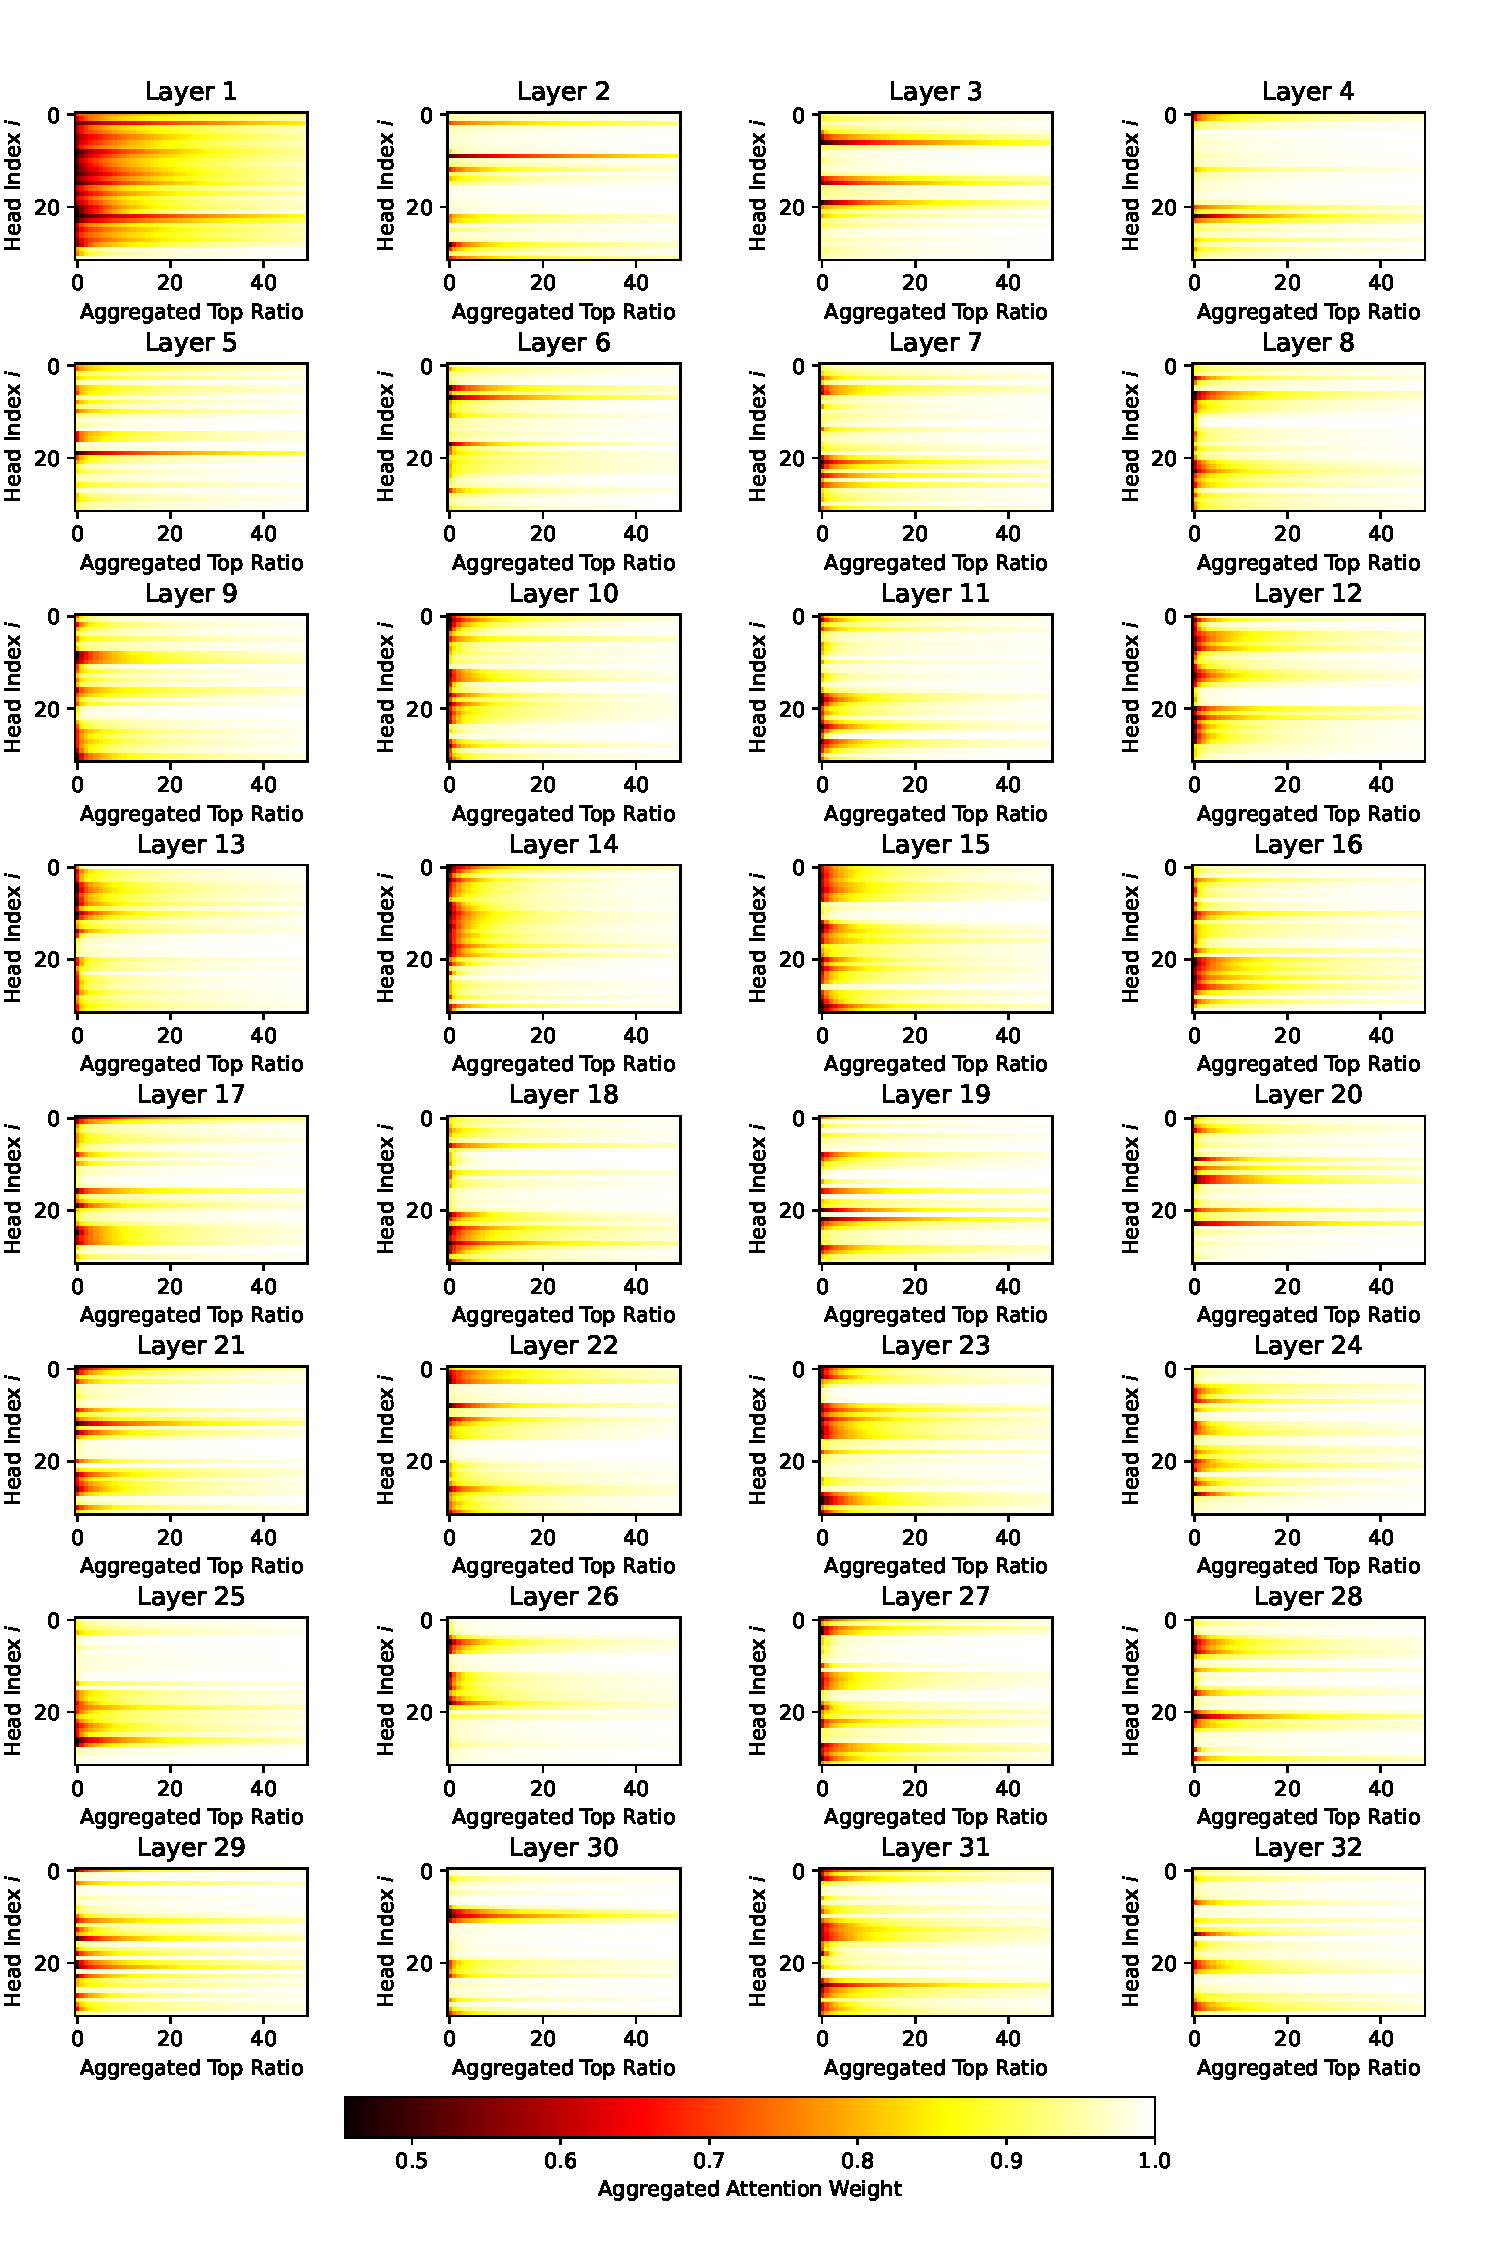
\includegraphics[width=0.8\textwidth]{./Figures/cusum_weight_all_layers.pdf}
	\caption{ Visualization of Heads' Concentrations}
	\label{fig:all_layers}
\end{figure*}




\begin{table*}[h]
	\small
	\centering
	\caption{S-NIAH and MK-NIAH templates in Ruler Benchmark.~\cite{hsieh2024ruler}}
	\label{tab:ruler_task_template1}
	\resizebox{\linewidth}{!}{
		\begin{tabular}{cp{0.9\linewidth}}
			\toprule
			
			\begin{tabular}{@{}c@{}}Single NIAH\\Subtask-1 \\(S-NIAH-1)\end{tabular} & 
			\begin{tabular}{@{}p{\linewidth}@{}} 
				\textbf{Task Template:} \\
				Some special magic numbers are hidden within the following text. Make sure to memorize it. I will quiz you about the numbers afterwards.\\
				\textcolor{lightgray}{The grass is green. The sky is blue. The sun is yellow. Here we go. There and back again.} \\
				\textcolor{lightgray}{......} One of the special magic numbers for \textcolor{violet}{\{word\}} is: \textcolor{orange}{\{number\}}. \textcolor{lightgray}{......}\\
				% What is the special magic number for \textcolor{violet}{\{word\}} mentioned in the provided text? \\ \\
				% \textbf{Task Answer Prefix:} \\
				% The special magic number for \textcolor{violet}{\{word\}} mentioned in the provided text is\end{tabular}\\
                \textcolor{question_color}{What is the special magic number for \{word\} mentioned in the provided text?} \\ \\
                \textcolor{question_color}{The special magic number for \{word\} mentioned in the provided text is}
            \end{tabular}\\
			
			\midrule
			
			\begin{tabular}{@{}c@{}}Single NIAH\\Subtask-2\\(S-NIAH-2)\end{tabular} & 
			\begin{tabular}{@{}p{\linewidth}@{}} 
				\textbf{Task Template:} \\
				Some special magic numbers are hidden within the following text. Make sure to memorize it. I will quiz you about the numbers afterwards.\\
				\textcolor{lightgray}{Paul Graham Essays.} \\
				\textcolor{lightgray}{......} One of the special magic numbers for \textcolor{violet}{\{word\}} is: \textcolor{orange}{\{number\}}. \textcolor{lightgray}{......}\\
				% What is the special magic number for \textcolor{violet}{\{word\}} mentioned in the provided text? \\ \\
				% \textbf{Task Answer Prefix:} \\
				% The special magic number for \textcolor{violet}{\{word\}} mentioned in the provided text is\end{tabular}\\
                \textcolor{question_color}{What is the special magic number for \{word\} mentioned in the provided text?} \\ \\
            \textcolor{question_color}{The special magic number for \{word\} mentioned in the provided text is}
            \end{tabular}\\
			
			\midrule
			
			% \begin{tabular}{@{}c@{}}S-NIAH\\task3\end{tabular} & 
			% \begin{tabular}{@{}p{\linewidth}@{}} 
				% \textbf{Task Template:} \\
				% Some special magic uuids are hidden within the following text. Make sure to memorize it. I will quiz you about the uuids afterwards.\\
				% \textcolor{lightgray}{Paul Graham Essays.} \\
				% \textcolor{lightgray}{......} One of the special magic uuids for \textcolor{violet}{\{word\}} is: \textcolor{orange}{\{UUID\}}. \textcolor{lightgray}{......}\\
				% What is the special magic uuid for \textcolor{violet}{\{word\}} mentioned in the provided text? \\ \\
				% \textbf{Task Answer Prefix:} \\
				% The special magic uuid for \textcolor{violet}{\{word\}} mentioned in the provided text is\end{tabular}\\
			
			% \midrule
			
			\begin{tabular}{@{}c@{}}Single NIAH\\Subtask-3\\(S-NIAH-3)\end{tabular} & 
			\begin{tabular}{@{}p{\linewidth}@{}} 
				\textbf{Task Template:} \\
				Some special magic words are hidden within the following text. Make sure to memorize it. I will quiz you about the words afterwards.\\
				\textcolor{lightgray}{Paul Graham Essays.} \\
				\textcolor{lightgray}{......} One of the special magic words for \textcolor{violet}{\{word\}} is: \textcolor{orange}{\{word\}}. \textcolor{lightgray}{......}\\
				% What is the special magic word for \textcolor{violet}{\{word\}} mentioned in the provided text? \\ \\
				% \textbf{Task Answer Prefix:} \\
				% The special magic word for \textcolor{violet}{\{word\}} mentioned in the provided text is\end{tabular}\\
                \textcolor{question_color}{What is the special magic word for \{word\} mentioned in the provided text?} \\ \\
                \textcolor{question_color}{The special magic word for \{word\} mentioned in the provided text is}
            \end{tabular}\\
			
			\midrule
			
			\begin{tabular}{@{}c@{}}Multi-keys NIAH\\Subtask-1\\(MK-NIAH-1)\end{tabular} & 
			\begin{tabular}{@{}p{\linewidth}@{}} 
				\textbf{Task Template:} \\
				Some special magic numbers are hidden within the following text. Make sure to memorize it. I will quiz you about the numbers afterwards.\\
				\textcolor{lightgray}{Paul Graham Essays.} \\
				\textcolor{lightgray}{......} \textcolor{lightgray}{One of the special magic numbers for \{word-1\} is: \{number-1\}.} \textcolor{lightgray}{......}\\
				\textcolor{lightgray}{......} \textcolor{lightgray}{One of the special magic numbers for \{word-2\} is: \{number-2\}.} \textcolor{lightgray}{......}\\
				\textcolor{lightgray}{......} \textcolor{lightgray}{One of the special magic numbers for \{word-3\} is: \{number-3\}.} \textcolor{lightgray}{......}\\
				\textcolor{lightgray}{......} One of the special magic numbers for \textcolor{violet}{\{word-4\}} is: \textcolor{orange}{\{number-4\}}. \textcolor{lightgray}{......}\\
				% What is the special magic number for \textcolor{violet}{\{word-4\}} mentioned in the provided text? \\ \\
				% \textbf{Task Answer Prefix:} \\
				% The special magic number for \textcolor{violet}{\{word-4\}} mentioned in the provided text is\end{tabular}\\
                \textcolor{question_color}{What is the special magic number for \{word-4\} mentioned in the provided text?} \\ \\
                \textcolor{question_color}{The special magic number for \{word-4\} mentioned in the provided text is}
            \end{tabular}\\
			
			\midrule
			
			\begin{tabular}{@{}c@{}}Multi-keys NIAH\\Subtask-2\\(MK-NIAH-2)\end{tabular} & 
			\begin{tabular}{@{}p{\linewidth}@{}} 
				\textbf{Task Template:} \\
				Some special magic numbers are hidden within the following text. Make sure to memorize it. I will quiz you about the numbers afterwards.\\
				\textcolor{lightgray}{One of the special magic numbers for \{word-1\} is: \{number-1\}.} \\
				\textcolor{lightgray}{One of the special magic numbers for \{word-2\} is: \{number-2\}.} \\
				\textcolor{lightgray}{......} One of the special magic numbers for \textcolor{violet}{\{word-x\}} is: \textcolor{orange}{\{number-x\}}. \textcolor{lightgray}{......}\\
				\textcolor{lightgray}{One of the special magic numbers for \{word-n-1\} is: \{number-n-1\}.} \\
				\textcolor{lightgray}{One of the special magic numbers for \{word-n\} is: \{number-n\}.} \\
				% What is the special magic number for \textcolor{violet}{\{word-x\}} mentioned in the provided text? \\ \\
				% \textbf{Task Answer Prefix:} \\
				% The special magic number for \textcolor{violet}{\{word-x\}} mentioned in the provided text is\end{tabular}\\
                \textcolor{question_color}{What is the special magic number for \{word-x\} mentioned in the provided text?} \\ \\
                \textcolor{question_color}{The special magic number for \{word-x\} mentioned in the provided text is}
            \end{tabular}\\
			
			\midrule
			
			\begin{tabular}{@{}c@{}}Multi-keys NIAH\\Subtask-3\\(MK-NIAH-3)\end{tabular} & 
			\begin{tabular}{@{}p{\linewidth}@{}} 
				\textbf{Task Template:} \\
				Some special magic uuids are hidden within the following text. Make sure to memorize it. I will quiz you about the uuids afterwards.\\
				\textcolor{lightgray}{One of the special magic uuids for \{uuid-1\} is: \{uuid-1\}.} \\
				\textcolor{lightgray}{One of the special magic uuids for \{uuid-2\} is: \{uuid-2\}.} \\
				\textcolor{lightgray}{......} One of the special magic uuids for \textcolor{violet}{\{uuid-x\}} is: \textcolor{orange}{\{uuid-x\}}. \textcolor{lightgray}{......}\\
				\textcolor{lightgray}{One of the special magic uuids for \{uuid-n-1\} is: \{uuid-n-1\}.} \\
				\textcolor{lightgray}{One of the special magic uuids for \{uuid-n\} is: \{uuid-n\}.} \\
				% What is the special magic number for \textcolor{violet}{\{uuid-x\}} mentioned in the provided text? \\ \\
				% \textbf{Task Answer Prefix:} \\
				% The special magic number for \textcolor{violet}{\{uuid-x\}} mentioned in the provided text is\end{tabular}\\
                \textcolor{question_color}{What is the special magic number for \{uuid-x\} mentioned in the provided text?} \\ \\
                \textcolor{question_color}{The special magic number for \{uuid-x\} mentioned in the provided text is}
            \end{tabular}\\
			
			
			\bottomrule
	\end{tabular}}
\end{table*}


\begin{table*}[h]
	\small
	\centering
	\caption{MV-NIAH, MQ-NIAH, VT, CWE, and FWE templates in Ruler Benchmark.~\cite{hsieh2024ruler}}
	\label{tab:ruler_task_template2}
	\resizebox{\linewidth}{!}{
		\begin{tabular}{cp{0.9\linewidth}}
			\toprule
			
			% \begin{tabular}{@{}c@{}}MV-NIAH\\Subtask-1\end{tabular} & 
			% \begin{tabular}{@{}p{\linewidth}@{}} 
				% \textbf{Task Template:} \\
				% Some special magic numbers are hidden within the following text. Make sure to memorize it. I will quiz you about the numbers afterwards.\\
				% \textcolor{lightgray}{Paul Graham Essays...} \\
				% \textcolor{lightgray}{......} One of the special magic numbers for \textcolor{violet}{\{word\}} is: \textcolor{orange}{\{number-1\}}. \textcolor{lightgray}{......}\\
				% \textcolor{lightgray}{......} One of the special magic numbers for \textcolor{violet}{\{word\}} is: \textcolor{orange}{\{number-2\}}. \textcolor{lightgray}{......}\\
				% What are all the special magic numbers for \textcolor{violet}{\{word\}} mentioned in the provided text? \\ \\
				% \textbf{Task Answer Prefix:} \\
				% The special magic numbers for \textcolor{violet}{\{word\}} mentioned in the provided text are\end{tabular}\\
			
			% \midrule
			
			\begin{tabular}{@{}c@{}}Multi-values NIAH\\(MV-NIAH)\end{tabular} & 
			\begin{tabular}{@{}p{\linewidth}@{}} 
				\textbf{Task Template:} \\
				Some special magic numbers are hidden within the following text. Make sure to memorize it. I will quiz you about the numbers afterwards.\\
				\textcolor{lightgray}{Paul Graham Essays.} \\
				\textcolor{lightgray}{......} One of the special magic numbers for \textcolor{violet}{\{word\}} is: \textcolor{orange}{\{number-1\}}. \textcolor{lightgray}{......}\\
				\textcolor{lightgray}{......} One of the special magic numbers for \textcolor{violet}{\{word\}} is: \textcolor{orange}{\{number-2\}}. \textcolor{lightgray}{......}\\
				\textcolor{lightgray}{......} One of the special magic numbers for \textcolor{violet}{\{word\}} is: \textcolor{orange}{\{number-3\}}. \textcolor{lightgray}{......}\\
				\textcolor{lightgray}{......} One of the special magic numbers for \textcolor{violet}{\{word\}} is: \textcolor{orange}{\{number-4\}}. \textcolor{lightgray}{......}\\
				% What are all the special magic numbers for \textcolor{violet}{\{word\}} mentioned in the provided text? \\ \\
				% \textbf{Task Answer Prefix:} \\
				% The special magic numbers for \textcolor{violet}{\{word\}} mentioned in the provided text are\end{tabular}\\
                \textcolor{question_color}{What are all the special magic numbers for \{word\} mentioned in the provided text?} \\ \\
                \textcolor{question_color}{The special magic numbers for \{word\} mentioned in the provided text are}
            \end{tabular}\\
			
			\midrule
			
			% \begin{tabular}{@{}c@{}}MQ-NIAH\\Subtask-1\end{tabular} & 
			% \begin{tabular}{@{}p{\linewidth}@{}} 
				% \textbf{Task Template:} \\
				% Some special magic numbers are hidden within the following text. Make sure to memorize it. I will quiz you about the numbers afterwards.\\
				% \textcolor{lightgray}{Paul Graham Essays.} \\
				% \textcolor{lightgray}{......} One of the special magic numbers for \textcolor{violet}{\{word-1\}} is: \textcolor{orange}{\{number-1\}}. \textcolor{lightgray}{......} \\
				% \textcolor{lightgray}{......} One of the special magic numbers for \textcolor{violet}{\{word-2\}} is: \textcolor{orange}{\{number-2\}}. \textcolor{lightgray}{......}\\
				% What are all the special magic numbers for \textcolor{violet}{\{word-1\}} and \textcolor{violet}{\{word-2\}} mentioned in the provided text? \\ \\
				% \textbf{Task Answer Prefix:} \\
				% The special magic numbers for \textcolor{violet}{\{word-1\}} and \textcolor{violet}{\{word-2\}} mentioned in the provided text are\end{tabular}\\
			
			% \midrule
			
			\begin{tabular}{@{}c@{}}Multi-queries NIAH\\(MQ-NIAH)\end{tabular} & 
			\begin{tabular}{@{}p{\linewidth}@{}} 
				\textbf{Task Template:} \\
				Some special magic numbers are hidden within the following text. Make sure to memorize it. I will quiz you about the numbers afterwards.\\
				\textcolor{lightgray}{Paul Graham Essays.} \\
				\textcolor{lightgray}{......} One of the special magic numbers for \textcolor{violet}{\{word-1\}} is: \textcolor{orange}{\{number-1\}}. \textcolor{lightgray}{......} \\    
				\textcolor{lightgray}{......} One of the special magic numbers for \textcolor{violet}{\{word-2\}} is: \textcolor{orange}{\{number-2\}}. \textcolor{lightgray}{......} \\
				\textcolor{lightgray}{......} One of the special magic numbers for \textcolor{violet}{\{word-3\}} is: \textcolor{orange}{\{number-3\}}. \textcolor{lightgray}{......} \\
				\textcolor{lightgray}{......} One of the special magic numbers for \textcolor{violet}{\{word-4\}} is: \textcolor{orange}{\{number-4\}}. \textcolor{lightgray}{......}\\
				% What are all the special magic numbers for \textcolor{violet}{\{word-1\}}, \textcolor{violet}{\{word-2\}}, \textcolor{violet}{\{word-3\}}, and \textcolor{violet}{\{word-4\}} mentioned in the provided text? \\ \\
				% \textbf{Task Answer Prefix:} \\
				% The special magic numbers for \textcolor{violet}{\{word-1\}}, \textcolor{violet}{\{word-2\}}, \textcolor{violet}{\{word-3\}}, and \textcolor{violet}{\{word-4\}} mentioned in the provided text are\end{tabular}\\
                \textcolor{question_color}{What are all the special magic numbers for \{word-1\}, \{word-2\}, \{word-3\}, and \{word-4\} mentioned in the provided text?} \\ \\
                \textcolor{question_color}{The special magic numbers for \{word-1\}, \{word-2\}, \{word-3\}, and \{word-4\} mentioned in the provided text are}
            \end{tabular}\\
			
			\midrule
			
			\begin{tabular}{@{}c@{}}Variable Tracking\\(VT)\end{tabular} & 
			\begin{tabular}{@{}p{\linewidth}@{}} 
				\textbf{Task Template:} \\
				\textcolor{blue}{\{one task example\}} \\
				Memorize and track the chain(s) of variable assignment hidden in the following text.\\\\
				\textcolor{lightgray}{The grass is green. The sky is blue. The sun is yellow. Here we go. There and back again.}
				\textcolor{lightgray}{......} VAR \textcolor{orange}{\{X1\}} = \textcolor{violet}{\{number\}} \textcolor{lightgray}{......}\\
				\textcolor{lightgray}{......} VAR \textcolor{orange}{\{X2\}} = \textcolor{orange}{\{X1\}} \textcolor{lightgray}{......}\\
				\textcolor{lightgray}{......} VAR \textcolor{orange}{\{X3\}} = \textcolor{orange}{\{X2\}} \textcolor{lightgray}{......}\\
				\textcolor{lightgray}{......} VAR \textcolor{orange}{\{X4\}} = \textcolor{orange}{\{X3\}} \textcolor{lightgray}{......}\\
				\textcolor{lightgray}{......} VAR \textcolor{orange}{\{X5\}} = \textcolor{orange}{\{X4\}} \textcolor{lightgray}{......}\\
				% Question: Find all variables that are assigned the value \textcolor{violet}{\{number\}} in the text above. \\\\
				% \textbf{Task Answer Prefix:} \\
				% Answer: According to the chain(s) of variable assignment in the text above, 5 variables are assigned the value \textcolor{violet}{\{number\}}, they are: 
                \textcolor{question_color}{Question: Find all variables that are assigned the value \{number\} in the text above.} \\\\
                \textcolor{question_color}{Answer: According to the chain(s) of variable assignment in the text above, 5 variables are assigned the value \{number\}, they are: }
			\end{tabular}\\
			
			\midrule
			
			\begin{tabular}{@{}c@{}}Common Words Extraction\\(CWE)\end{tabular} & 
			\begin{tabular}{@{}p{\linewidth}@{}} 
				\textbf{Task Template:} \\
				\textcolor{blue}{\{one task example\}} \\
				Below is a numbered list of words. In these words, some appear more often than others. Memorize the ones that appear most often.\\
				1. \textcolor{orange}{word-a} 2. \textcolor{lightgray}{word-b} 3. \textcolor{lightgray}{word-c} 4. \textcolor{orange}{word-a} 5. \textcolor{lightgray}{word-d} 6. \textcolor{orange}{word-a} 7. \textcolor{lightgray}{word-e} 8. \textcolor{lightgray}{word-f} \textcolor{lightgray}{......}\\
				% Question: What are the 10 most common words in the above list? \\\\
				% \textbf{Task Answer Prefix:} \\
				% Answer: The top 10 words that appear most often in the list are: 
                \textcolor{question_color}{Question: What are the 10 most common words in the above list?} \\\\
                \textcolor{question_color}{Answer: The top 10 words that appear most often in the list are: }
			\end{tabular}\\
			
			\midrule
			
			\begin{tabular}{@{}c@{}}Frequent Words Extraction\\(FWE)\end{tabular} & 
			\begin{tabular}{@{}p{\linewidth}@{}} 
				\textbf{Task Template:} \\
				Read the following coded text and track the frequency of each coded word. Find the three most frequently appeared coded words. \textcolor{lightgray}{... ...} \textcolor{orange}{word-a} \textcolor{lightgray}{... word-b ... ... ... word-c ...} \textcolor{orange}{word-a} \textcolor{lightgray}{... word-d word-e ...} \textcolor{orange}{word-a} \textcolor{lightgray}{... ... word-f ... ... ... ... word-g ... word-h ...} \textcolor{orange}{word-a} \textcolor{lightgray}{... word-i ......} \\
				% Question: Do not provide any explanation. Please ignore the dots '....'. What are the three most frequently appeared words in the above coded text? \\\\
				% \textbf{Task Answer Prefix:} \\
				% Answer: According to the coded text above, the three most frequently appeared words are:
                \textcolor{question_color}{Question: Do not provide any explanation. Please ignore the dots '....'. What are the three most frequently appeared words in the above coded text?} \\\\
                \textcolor{question_color}{Answer: According to the coded text above, the three most frequently appeared words are:}
			\end{tabular}\\
			
			\bottomrule
	\end{tabular}}
\end{table*}


\begin{table*}[h]
	\small
	\centering
	\caption{QA templates in Ruler Benchmark.~\cite{hsieh2024ruler}}
	\label{tab:ruler_task_template3}
	\resizebox{\linewidth}{!}{
		\begin{tabular}{cp{0.9\linewidth}}
			\toprule
			
			\begin{tabular}{@{}c@{}}Single\\Hop QA\\(S-QA)\end{tabular} & 
			\begin{tabular}{@{}p{\linewidth}@{}} 
				\textbf{Task Template:} \\
				Answer the question based on the given documents. Only give me the answer and do not output any other words.\\\\
				The following are given documents.\\\\
				\textcolor{lightgray}{Document 1:} \\ \textcolor{lightgray}{\{document-1\}} \\
				\textcolor{lightgray}{......} \\
				\textcolor{violet}{Document x:} \\ \textcolor{orange}{\{document-x\}} \\
				\textcolor{lightgray}{......} \\
				\textcolor{lightgray}{Document n:} \\ \textcolor{lightgray}{\{document-n\}} \\\\
				
				% Answer the question based on the given documents. Only give me the answer and do not output any other words.\\\\
				% Question: \textcolor{violet}{question}\\\\
				% \textbf{Task Answer Prefix:} \\
				% Answer: 
                \textcolor{question_color}{Answer the question based on the given documents. Only give me the answer and do not output any other words.}\\\\
                \textcolor{question_color}{Question: \{question\}}\\\\
                \textcolor{question_color}{Answer: }
			\end{tabular}\\
			
			\midrule
			
			\begin{tabular}{@{}c@{}}Multi\\Hop QA\\(M-QA)\end{tabular} & 
			\begin{tabular}{@{}p{\linewidth}@{}} 
				\textbf{Task Template:} \\
				Answer the question based on the given documents. Only give me the answer and do not output any other words.\\\\
				The following are given documents.\\\\
				\textcolor{lightgray}{Document 1:} \\ \textcolor{lightgray}{\{document-1\}} \\
				\textcolor{lightgray}{......} \\
				\textcolor{violet}{Document x:} \\ \textcolor{orange}{\{document-x\}} \\
				\textcolor{lightgray}{......} \\
				\textcolor{violet}{Document y:} \\ \textcolor{orange}{\{document-y\}} \\
				\textcolor{lightgray}{......} \\
				\textcolor{lightgray}{Document n:} \\ \textcolor{lightgray}{\{document-n\}} \\\\
				
				% Answer the question based on the given documents. Only give me the answer and do not output any other words.\\\\
				% Question: \textcolor{violet}{question}\\\\
				% \textbf{Task Answer Prefix:} \\
				% Answer: 
                \textcolor{question_color}{Answer the question based on the given documents. Only give me the answer and do not output any other words.}\\\\
                \textcolor{question_color}{Question: \{question\}}\\\\
                \textcolor{question_color}{Answer: }
			\end{tabular}\\
			
			\bottomrule
	\end{tabular}}
\end{table*}



\begin{table*}[thb!]
	\centering
	\caption{Details of 16 Datasets in LongBench}
	\label{tab:information_dataset}
	 \resizebox{\textwidth}{!}{%
		\begin{tabular}{@{}llllrlr@{}}
			\toprule
			Label     & Task                & Task Type     & Eval metric & Avg len & Language & Sample Num        \\ \midrule
			NrtvQA    & NarrativeQA         & Single-Doc. QA & F1          & 18,409   & EN       & 200            \\
			Qasper     & Qasper              & Single-Doc. QA & F1          & 3,619    & EN       & 200            \\
			MF-en     & MultiFieldQA-en     & Single-Doc. QA & F1          & 4,559    & EN       & 150            \\
			HotpotQA  & HotpotQA            & Multi-Doc. QA  & F1          & 9,151    & EN       & 200            \\
			2WikiMQA  & 2WikiMultihopQA     & Multi-Doc. QA  & F1          & 4,887    & EN       & 200            \\
			Musique   & MuSiQue             & Multi-Doc. QA  & F1          & 11,214   & EN       & 200            \\
			GovReport & GovReport           & Summarization & Rouge-L     & 8,734    & EN       & 200            \\
			QMSum     & QMSum               & Summarization & Rouge-L     & 10,614   & EN       & 200            \\
			MultiNews & MultiNews           & Summarization & Rouge-L     & 2,113    & EN       & 200            \\
			TREC      & TREC                & Few-shotLearning      & Accuracy    & 5,177    & EN       & 200            \\
			TriviaQA  & TriviaQA            & Few-shotLearning      & F1          & 8,209    & EN       & 200            \\
			SAMSum    & SAMSum              & Few-shotLearning      & Rouge-L     & 6,258    & EN       & 200            \\
			PCount    & PassageCount        & Synthetic     & Accuracy    & 11,141   & EN       & 200            \\
			PRe       & PassageRetrieval-en & Synthetic     & Accuracy    & 9,289    & EN       & 200            \\
			Lcc       & LCC                 & Code          & Edit Sim    & 1,235      & Python/C\#/Java & 500\\
			RB-P      & RepoBench-P         & Code          & Edit Sim    & 4,206      & Python/Java & 500    \\ \bottomrule
		\end{tabular}%
		}
\end{table*}


\begin{table*}[h]
	\small
	\centering
	\caption{LongBench templates. Single-Doc. QA Tasks.}
	\label{tab:longbenc_template_1}
	\resizebox{\linewidth}{!}{
		\begin{tabular}{cp{0.9\linewidth}}
			\toprule
			
			\begin{tabular}{@{}c@{}}NarrativeQA\end{tabular} & 
			\begin{tabular}{@{}p{\linewidth}@{}} 
				\textbf{Task Template:} \\
				
				You are given a story, which can be either a novel or a movie script, and a question. Answer the question asconcisely as you can, using a single phrase if possible. Do not provide any explanation. \\\\
				Story: \textcolor{orange}{\{context\}} \\\\
				
				\textcolor{question_color}{Now, answer the question based on the story asconcisely as you can, using a single phrase if possible. Do not provide any explanation.}\\\\
				
				\textcolor{question_color}{Question: \textcolor{question_color}{\{question\}}}\\
				
				% \textbf{Task Answer Prefix:} \\
				% Answer: 
			\end{tabular}\\
			
			
			\midrule
			
			\begin{tabular}{@{}c@{}}Qasper\end{tabular} & 
			\begin{tabular}{@{}p{\linewidth}@{}} 
				\textbf{Task Template:} \\
				
				You are given a scientific article and a question. Answer the question as concisely as you can, using a single phrase or sentence if possible. If the question cannot be answered based on the information in the article, write "unanswerable". If the question is a yes/no question, answer "yes", "no", or "unanswerable". Do not provide any explanation.\\\\
				Article: \textcolor{orange}{\{context\}}\\\\
				\textcolor{question_color}{Answer the question based on the above article as concisely as you can, using a single phrase or sentence if possible. If the question cannot be answered based on the information in the article, write "unanswerable". If the question is a yes/no question, answer "yes", "no", or "unanswerable". Do not provide any explanation.}\\\\
				\textcolor{question_color}{Question: \textcolor{question_color}{\{question\}}}\\
				
				% \textbf{Task Answer Prefix:} \\
				% Answer: 
			\end{tabular}\\
			
			
			\midrule
			
			\begin{tabular}{@{}c@{}}MultifieldQA EN\end{tabular} & 
			\begin{tabular}{@{}p{\linewidth}@{}} 
				\textbf{Task Template:} \\
				
				Read the following text and answer briefly.\\\\
				\textcolor{orange}{\{context\}}\\\\
				\textcolor{question_color}{Now, answer the following question based on the above text, only give me the answer and do not output any other words.}\\\\
				\textcolor{question_color}{Question: \textcolor{question_color}{\{question\}}} \\
				% \textbf{Task Answer Prefix:} \\
				% Answer: 
			\end{tabular}\\
			
			
			\bottomrule
	\end{tabular}}
\end{table*}


\begin{table*}[h]
	\small
	\centering
	\caption{LongBench templates. Multi-Doc. QA Tasks.}
	\label{tab:longbenc_template_2}
	\resizebox{\linewidth}{!}{
		\begin{tabular}{cp{0.9\linewidth}}
			\toprule
			
			\begin{tabular}{@{}c@{}}HotpotQA\end{tabular} & 
			\begin{tabular}{@{}p{\linewidth}@{}} 
				\textbf{Task Template:} \\
				
				Answer the question based on the given passages. Only give me the answer and do not output any other words.\\\\
				The following are given passages.\\
				\textcolor{orange}{\{context\}}\\\\
				\textcolor{question_color}{Answer the question based on the given passages. Only give me the answer and do not output any other words.}\\\\
				\textcolor{question_color}{Question: \textcolor{question_color}{\{question\}}} \\
				
				% \textbf{Task Answer Prefix:} \\
				% Answer: 
			\end{tabular}\\
			
			
			\midrule
			
			\begin{tabular}{@{}c@{}}2WikimQA\end{tabular} & 
			\begin{tabular}{@{}p{\linewidth}@{}} 
				\textbf{Task Template:} \\
				
				Answer the question based on the given passages. Only give me the answer and do not output any other words.\\\\
				The following are given passages.\\
				\textcolor{orange}{\{context\}}\\\\
				\textcolor{question_color}{Answer the question based on the given passages. Only give me the answer and do not output any other words.}\\\\
				\textcolor{question_color}{Question: \textcolor{question_color}{\{question\}}}
				
				% \textbf{Task Answer Prefix:} \\
				% Answer: 
			\end{tabular}\\
			
			
			\midrule
			
			\begin{tabular}{@{}c@{}}Musique\end{tabular} & 
			\begin{tabular}{@{}p{\linewidth}@{}} 
				\textbf{Task Template:} \\
				
				Answer the question based on the given passages. Only give me the answer and do not output any other words.\\\\
				The following are given passages.\\
				\textcolor{orange}{\{context\}}\\\\
				\textcolor{question_color}{Answer the question based on the given passages. Only give me the answer and do not output any other words.}\\\\
				\textcolor{question_color}{Question: \textcolor{question_color}{\{question\}}}
				
				% \textbf{Task Answer Prefix:} \\
				% Answer: 
			\end{tabular}\\
			
			%%%%%%%%%%%%%%%%%%%%%%%%
			\bottomrule
	\end{tabular}}
\end{table*}


\begin{table*}[h]
	\small
	\centering
	\caption{LongBench templates. Summarization Tasks.}
	\label{tab:longbenc_template_3}
	\resizebox{\linewidth}{!}{
		\begin{tabular}{cp{0.9\linewidth}}
			\toprule
			
			\begin{tabular}{@{}c@{}}Gov Report\end{tabular} & 
			\begin{tabular}{@{}p{\linewidth}@{}} 
				\textbf{Task Template:} \\
				
				You are given a report by a government agency. Write a one-page summary of the report.\\\\
				Report:\\
				\textcolor{orange}{\{context\}}\\\\
				\textcolor{question_color}{Now, write a one-page summary of the report.} \\
				% \textbf{Task Answer Prefix:} \\
				% Summary: 
			\end{tabular}\\
			
			
			\midrule
			
			\begin{tabular}{@{}c@{}}QMSum\end{tabular} & 
			\begin{tabular}{@{}p{\linewidth}@{}} 
				\textbf{Task Template:} \\
				
				You are given a meeting transcript and a query containing a question or instruction. Answer the query in one or more sentences.\\\\
				Transcript:\\
				\textcolor{orange}{\{context\}}\\\\
				\textcolor{question_color}{Now, answer the query based on the above meeting transcript in one or more sentences.}\\\\
				\textcolor{question_color}{Query: \textcolor{question_color}{\{question\}}} \\
				% \textbf{Task Answer Prefix:} \\
				% Answer:
			\end{tabular}\\
			
			
			
			\midrule
			
			\begin{tabular}{@{}c@{}}Multi News\end{tabular} & 
			\begin{tabular}{@{}p{\linewidth}@{}} 
				\textbf{Task Template:} \\
				
				You are given several news passages. Write a one-page summary of all news. \\\\
				News:\\
				\textcolor{orange}{\{context\}}\\\\
				\textcolor{question_color}{Now, write a one-page summary of all the news.}\\
				% \textbf{Task Answer Prefix:} \\
				% Summary:
			\end{tabular}\\
			
			
			%%%%%%%%%%%%%%%%%%%%%%%%
			\bottomrule
	\end{tabular}}
\end{table*}


\begin{table*}[h]
	\small
	\centering
	\caption{LongBench templates. Few-shot Learning Tasks.}
	\label{tab:longbenc_template_4}
	\resizebox{\linewidth}{!}{
		\begin{tabular}{cp{0.9\linewidth}}
			\toprule
			
			
			\begin{tabular}{@{}c@{}}TREC\end{tabular} & 
			\begin{tabular}{@{}p{\linewidth}@{}} 
				\textbf{Task Template:} \\
				
				Please determine the type of the question below. Here are some examples of questions.\\\\
				\textcolor{orange}{\{context\}}\\
				% \textcolor{violet}{\{question\}} \\
				\textcolor{question_color}{\{question\}} \\
				% \textbf{Task Answer Prefix:} \\
				
			\end{tabular}\\
			
			
			\midrule
			
			\begin{tabular}{@{}c@{}}TriviaQA\end{tabular} & 
			\begin{tabular}{@{}p{\linewidth}@{}} 
				\textbf{Task Template:} \\
				
				Answer the question based on the given passage. Only give me the answer and do not output any other words. The following are some examples.\\\\
				\textcolor{orange}{\{context\}}\\\\
				% \textcolor{violet}{\{question\}} \\
				\textcolor{question_color}{\{question\}} \\
				% \textbf{Task Answer Prefix:} \\
				
			\end{tabular}\\
			
			
			
			\midrule
			
			\begin{tabular}{@{}c@{}}SAMSum\end{tabular} & 
			\begin{tabular}{@{}p{\linewidth}@{}} 
				\textbf{Task Template:} \\
				
				Summarize the dialogue into a few short sentences. The following are some examples.\\\\
				\textcolor{orange}{\{context\}}\\\\
				% \textcolor{violet}{\{question\}} \\
				\textcolor{question_color}{\{question\}} \\
				% \textbf{Task Answer Prefix:} \\
			\end{tabular}\\
			
			
			%%%%%%%%%%%%%%%%%%%%%%%%
			\bottomrule
	\end{tabular}}
\end{table*}


\begin{table*}[h]
	\small
	\centering
	\caption{LongBench templates. Synthetic Tasks.}
	\label{tab:longbenc_template_5}
	\resizebox{\linewidth}{!}{
		\begin{tabular}{cp{0.9\linewidth}}
			\toprule
			
			
			\begin{tabular}{@{}c@{}}Passage Count\end{tabular} & 
			\begin{tabular}{@{}p{\linewidth}@{}} 
				\textbf{Task Template:} \\
				
				There are some paragraphs below sourced from Wikipedia. Some of them may be duplicates. Please carefully read these paragraphs and determine how many unique paragraphs there are after removing duplicates. In other words, how many non-repeating paragraphs are there in total?\\\\
				\textcolor{orange}{\{context\}}\\\\
				\textcolor{question_color}{Please enter the final count of unique paragraphs after removing duplicates. The output format should only contain the number, such as 1, 2, 3, and so on.}\\
				% \textbf{Task Answer Prefix:} \\
				% The final answer is: 
			\end{tabular}\\
			
			
			\midrule
			
			\begin{tabular}{@{}c@{}}Passage Retrieval EN\end{tabular} & 
			\begin{tabular}{@{}p{\linewidth}@{}} 
				\textbf{Task Template:} \\
				
				Here are 30 paragraphs from Wikipedia, along with an abstract. Please determine which paragraph the abstract is from.\\\\
				\textcolor{orange}{\{context\}}\\\\
				The following is an abstract.\\\\
				\textcolor{question_color}{\{question\}}\\\\
				\textcolor{question_color}{Please enter the number of the paragraph that the abstract is from. The answer format must be like "Paragraph 1", "Paragraph 2", etc.}\\
				% \textbf{Task Answer Prefix:} \\
				% The answer is
			\end{tabular}\\
			
			
			
			%%%%%%%%%%%%%%%%%%%%%%%%
			\bottomrule
	\end{tabular}}
\end{table*}


\begin{table*}[h]
	\small
	\centering
	\caption{LongBench templates. Code Tasks.}
	\label{tab:longbenc_template_6}
	\resizebox{\linewidth}{!}{
		\begin{tabular}{cp{0.9\linewidth}}
			\toprule
			
			
			\begin{tabular}{@{}c@{}}Lcc\end{tabular} & 
			\begin{tabular}{@{}p{\linewidth}@{}} 
				\textbf{Task Template:} \\
				
				Please complete the code given below. \\
				\textcolor{orange}{\{context\}} \\
				\textcolor{question_color}{Next line of code:}
				% \textbf{Task Answer Prefix:} \\
				% Next line of code:
			\end{tabular}\\
			
			\midrule
			
			\begin{tabular}{@{}c@{}}Repobench-P\end{tabular} & 
			\begin{tabular}{@{}p{\linewidth}@{}} 
				\textbf{Task Template:} \\
				
				Please complete the code given below. \\
				\textcolor{orange}{\{context\}} \\
				% \textcolor{violet}{\{question\}} \\
				\textcolor{question_color}{\{question\}} \\
				\textcolor{question_color}{Next line of code:}
				% \textbf{Task Answer Prefix:} \\
				% Next line of code:
			\end{tabular}\\
			
			%%%%%%%%%%%%%%%%%%%%%%%%
			
			\bottomrule
	\end{tabular}}
\end{table*}

\FloatBarrier


